\documentclass[10pt,openany]{book}
\usepackage{iftex}
\ifPDFTeX
\usepackage[utf8]{inputenc}
\DeclareUnicodeCharacter{2212}{\ensuremath{-}}
\DeclareUnicodeCharacter{2192}{\ensuremath{\to}}
\DeclareUnicodeCharacter{03B1}{\ensuremath{\alpha}}
\DeclareUnicodeCharacter{2248}{\ensuremath{\approx}}
\DeclareUnicodeCharacter{00D7}{\ensuremath{\times}}
\DeclareUnicodeCharacter{0394}{\ensuremath{\Delta}}
\DeclareUnicodeCharacter{2074}{\ensuremath{^4}}
\fi
\usepackage[T1]{fontenc}
\usepackage{lmodern}
\AtBeginDocument{\normalfont\DeclareFontShape{T1}{lmr}{bx}{sc}{<->ssub*lmr/m/sc}{}}
\usepackage[spanish,es-nodecimaldot]{babel}
\spanishplainpercent
\AtBeginDocument{\spanishdeactivate{"~<>}}
\usepackage[a4paper,margin=2.5cm,headheight=14pt]{geometry}
\usepackage{needspace}
\usepackage{amsmath,amssymb,mathtools,booktabs,array,longtable,graphicx,xcolor,tikz,enumitem,microtype,titlesec,fancyhdr}
\usepackage[breakable,skins]{tcolorbox}
\usepackage[labelfont=bf]{caption}
\usepackage[hyphens]{url}
\usepackage[hidelinks,unicode,hypertexnames=false]{hyperref}
\definecolor{studiumInk}{RGB}{20,44,64}
\definecolor{studiumBlue}{RGB}{24,74,130}
\definecolor{studiumCyan}{RGB}{0,184,205}
\definecolor{studiumLight}{RGB}{232,240,250}
\definecolor{studiumWorkedBack}{RGB}{255,244,230}
\definecolor{studiumWorkedFrame}{RGB}{138,78,12}
\definecolor{studiumCheckBack}{RGB}{243,236,248}
\definecolor{studiumCheckFrame}{RGB}{96,48,130}
\titleformat{\chapter}[display]{\normalfont\filright}{\large\mdseries\scshape\chaptertitlename\ \thechapter}{1ex}{\normalfont\huge\bfseries}
\titlespacing*{\chapter}{0pt}{2.5ex plus 1ex minus .2ex}{2.3ex}
\titleformat{name=\chapter,numberless}[display]{\normalfont\filright}{}{0pt}{\normalfont\huge\bfseries}
\titleformat{\section}{\Large\bfseries}{\thesection}{.8em}{}
\titleformat{\subsection}{\large\bfseries}{\thesubsection}{.7em}{}
\makeatletter
\renewcommand*\l@section{\@dottedtocline{1}{1.5em}{3.5em}}
\renewcommand*\l@subsection{\@dottedtocline{2}{3.8em}{5em}}
\makeatother
\setcounter{secnumdepth}{2}\setcounter{tocdepth}{2}
\setlength{\parindent}{1.5em}\setlength{\parskip}{3pt plus .5pt}
\setlength{\emergencystretch}{1.5em}\raggedbottom
\setlist{itemsep=2pt,topsep=4pt,leftmargin=*}
\setlist[description]{style=nextline,leftmargin=0pt,labelwidth=0pt,labelindent=0pt}
\allowdisplaybreaks[2]
\graphicspath{{figures/}}
\newcommand{\Raire}{287.05287}
\newcommand{\gzero}{9.80665}
\tcbset{studiumcommon/.style={breakable,boxrule=.65pt,arc=.7pt,left=1.7mm,right=1.7mm,top=1.3mm,bottom=1.3mm,before skip=10pt,after skip=10pt,fonttitle=\bfseries}}
\newtcolorbox{studiumworked}[1]{studiumcommon,colback=studiumWorkedBack,colframe=studiumWorkedFrame,colbacktitle=studiumWorkedFrame,coltitle=white,title={#1}}
\newcommand{\objetivos}[1]{\par\noindent\textbf{Objetivos de aprendizaje.} \textit{#1}\par\medskip}
\newcommand{\caja}[2]{\begin{tcolorbox}[studiumcommon,colback=studiumLight,colframe=studiumBlue,colbacktitle=studiumBlue,coltitle=white,title={#1}]#2\end{tcolorbox}}
\newcommand{\resumen}[1]{\begin{tcolorbox}[studiumcommon,colback=studiumCheckBack,colframe=studiumCheckFrame,colbacktitle=studiumCheckFrame,coltitle=white,title=Resumen]#1\end{tcolorbox}}
\newcommand{\figura}[2]{\begin{figure}[tbp]\centering\includegraphics[width=.83\linewidth]{#1.pdf}\caption{#2}\label{fig:#1}\end{figure}\noindent La figura~\ref{fig:#1} ofrece una representación del modelo discutido.}
\pagestyle{fancy}\fancyhf{}
\fancyhead[LE]{\small\thepage\hspace{1.5em}\mdseries\scshape\nouppercase{\leftmark}}
\fancyhead[RO]{\small\mdseries\scshape\nouppercase{\rightmark}\hspace{1.5em}\thepage}
\renewcommand{\headrulewidth}{.4pt}\renewcommand{\footrulewidth}{0pt}
\fancypagestyle{plain}{\fancyhf{}\fancyfoot[C]{\small\thepage}\renewcommand{\headrulewidth}{0pt}}

% Retícula Studium unificada: cabecera blanca, fotografía a sangre y bloque azul.
\addto\captionsspanish{\renewcommand{\contentsname}{Índice}\renewcommand{\tablename}{Cuadro}\renewcommand{\listtablename}{Índice de cuadros}}
\numberwithin{equation}{chapter}
\let\cleardoublepage\clearpage
\fancyfoot[R]{\scriptsize\sffamily\color{studiumInk}En revisión}
\renewcommand{\chaptermark}[1]{\markboth{Capítulo \thechapter.\ #1}{}}
\renewcommand{\sectionmark}[1]{\markright{\thesection\ #1}}
\definecolor{studiumTipBack}{RGB}{232,244,236}
\definecolor{studiumTipFrame}{RGB}{27,107,58}
\newcommand{\consejo}[2]{\begin{tcolorbox}[studiumcommon,colback=studiumTipBack,colframe=studiumTipFrame,colbacktitle=studiumTipFrame,coltitle=white,title={#1}]#2\end{tcolorbox}}
\newcommand{\estado}{Edición íntegra de estudio. Pendiente de revisión experta independiente.}
\newcommand{\portada}[3]{%
\hypersetup{pageanchor=false}
\begin{titlepage}\thispagestyle{empty}
\begin{tikzpicture}[remember picture,overlay,x=1bp,y=-1bp]
\begin{scope}[shift={(current page.north west)}]
\clip (0,0) rectangle (595.276,841.89);
\fill[white] (0,0) rectangle (595.276,841.89);
% Hero fotografico preencuadrado en la reticula de la coleccion (mismo
% borde superior y mismo bloque inferior que Teoria de Estructuras/Fluidos).
\node[anchor=north west,inner sep=0pt,outer sep=0pt] at (0,89.5)
  {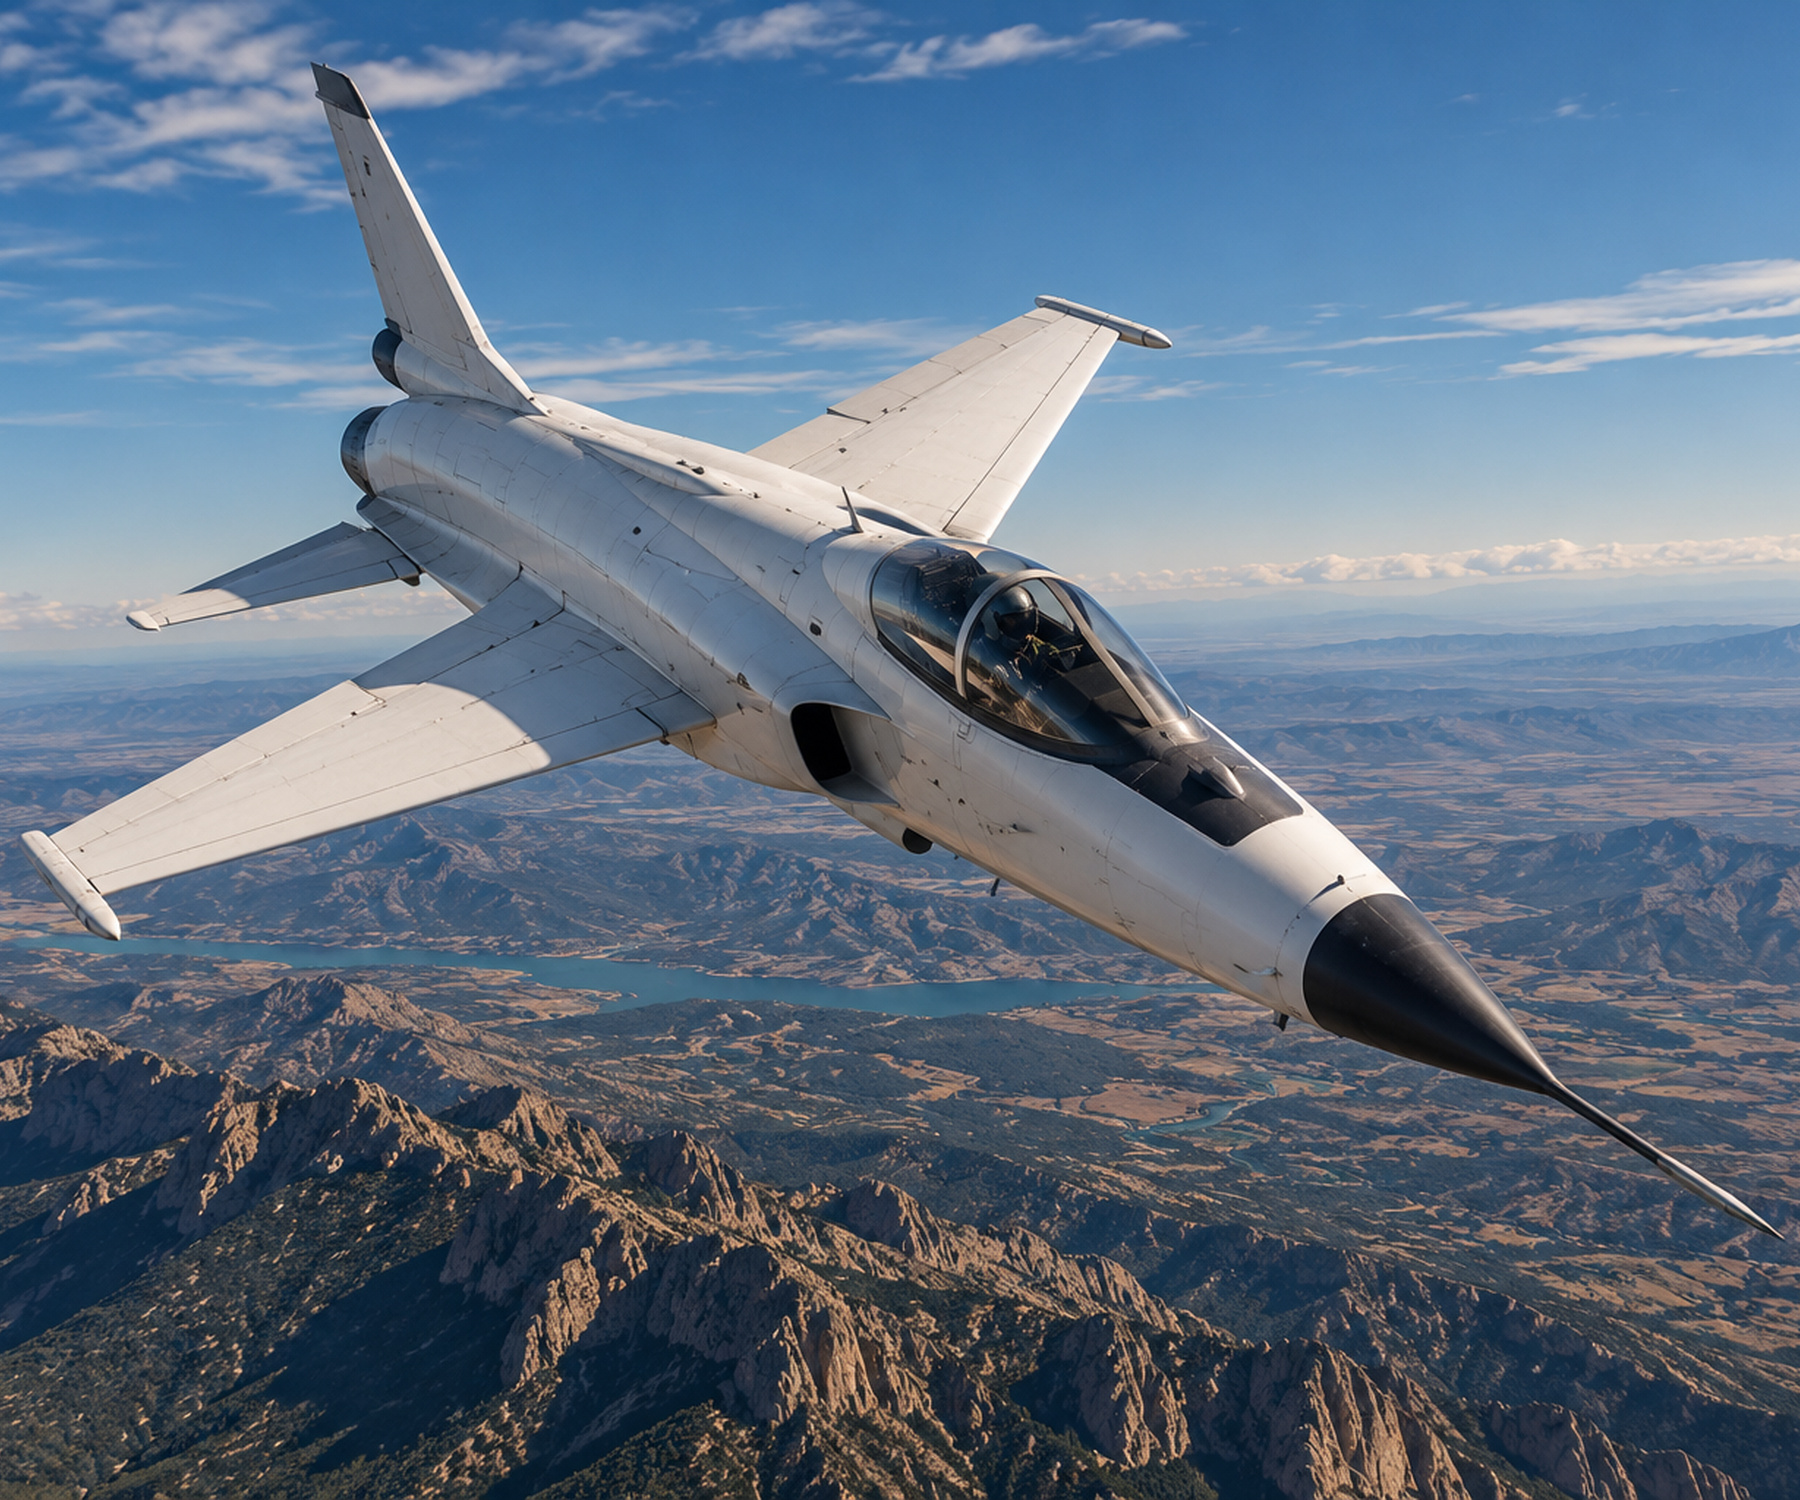
\includegraphics[width=595.276bp,height=496bp]{assets/cover-hero.jpg}};
\fill[studiumInk] (0,585.5) rectangle (595.276,841.89);
% Cabecera editorial.
% Logotipo auténtico de Studium: símbolo y letras extraídos sin redibujarlos
% de framework/docs/assets/studium-logo-dark.png, adaptados a una firma horizontal.
\node[anchor=north west,inner sep=0pt,outer sep=0pt] at (43,5)
  {
\includegraphics[width=185bp]{assets/studium-horizontal.png}};
\fill[studiumCyan] (106,76) rectangle (132,78);
\node[anchor=west,text=studiumInk,font=\sffamily\fontsize{8.2}{10}\selectfont,inner sep=0pt] at (140,79){BIBLIOTECA DE INGENIERÍA};
% Bloque inferior: tipografia, blancos y posiciones de la coleccion.
\node[anchor=west,text=studiumCyan,font=\sffamily\bfseries\fontsize{10}{12}\selectfont,inner sep=0pt] at (51.223,608){#1};
\node[anchor=north west,text=white,text width=493pt,font=\rmfamily\bfseries\fontsize{26.5}{29.5}\selectfont,inner sep=0pt] at (51.223,627){#2};
\node[anchor=north west,text=white!82!studiumInk,text width=493pt,font=\sffamily\fontsize{10}{13}\selectfont,inner sep=0pt] at (51.223,730){#3};
\node[anchor=west,text=white,font=\sffamily\bfseries\fontsize{10}{12}\selectfont,inner sep=0pt] at (51.223,774){GRADO EN INGENIERÍA AEROESPACIAL};
\node[anchor=west,text=white!82!studiumInk,font=\sffamily\fontsize{10}{12}\selectfont,inner sep=0pt] at (51.223,789){Universidad de León};
\draw[white!75!studiumInk,line width=.4pt] (51.223,801) -- (544.05,801);
\node[anchor=west,text=white!82!studiumInk,font=\sffamily\fontsize{10}{12}\selectfont,inner sep=0pt] at (51.223,822){2026};
\node[anchor=east,text=white,font=\sffamily\bfseries\fontsize{10}{12}\selectfont,inner sep=0pt] at (544.05,822){Primera edición};
\end{scope}\end{tikzpicture}\null
\end{titlepage}\hypersetup{pageanchor=true}}

\newcommand{\caso}[2]{\begin{studiumworked}{#1}#2\end{studiumworked}}
\newcommand{\ilustra}[2]{\begin{figure}[htbp]\centering\includegraphics[width=.94\linewidth]{#1.pdf}\caption{#2}\label{fig:#1}\end{figure}}
\newcommand{\fuentes}[1]{\par\medskip\noindent{\footnotesize\textbf{Fuentes y localizadores.} #1}\par}
\newcommand{\apartado}[2]{\par\medskip\noindent\textbf{#1.} #2\par}
\newcommand{\repaso}[2]{\par\medskip\noindent\textbf{Para comprobar la comprensión.} #1\par\noindent\textit{Respuesta razonada.} #2\par}

\newcommand{\vect}[1]{\boldsymbol{#1}}
\newcommand{\dd}{\mathrm{d}}
\newcommand{\SIu}[1]{\,\mathrm{#1}}
\newcommand{\hipotesis}[1]{\caja{Hipótesis y dominio}{#1}}
\newcommand{\verifica}[1]{\consejo{Comprobación y límites}{#1}}
\newcommand{\errorcomun}[1]{\caja{Error que cambia el resultado}{#1}}

\hypersetup{pdftitle={Mecánica de Vuelo},pdfauthor={Studium},pdfsubject={Dinámica, actuaciones y estabilidad de aeronaves}}
\begin{document}
\portada{MANUAL UNIVERSITARIO}{MECÁNICA DE VUELO}{Dinámica, actuaciones y estabilidad de aeronaves}
\frontmatter
\chapter*{Edición y alcance}
Manual original de estudio alineado con la guía docente pública de Mecánica de Vuelo, código 0710325, de la Universidad de León, curso 2026/2027. No es una publicación oficial de la Universidad ni sustituye las instrucciones de evaluación o los manuales operativos certificados.

\textbf{En revisión.} Las verificaciones reproducibles comprueban operaciones y modelos declarados. La revisión académica experta independiente permanece pendiente. La estabilidad dinámica se incorpora como ampliación del programa oficial de estabilidad estática.

% Copyright / artwork statement for the image actually embedded in all PDFs.
\noindent\textbf{Imagen de portada.} Ilustración aeronáutica fotorrealista,
original y generada digitalmente para esta edición independiente de Studium
(2026). Representa una aeronave en maniobra de alabeo sobre un paisaje
montañoso; no es una fotografía documental ni representa un avión concreto.
El diseño incorpora el logotipo original de Studium proporcionado con el
proyecto. No implica aval de la Universidad de León ni de ninguna institución.

 Las figuras, los ejemplos y los ejercicios han sido elaborados para esta edición. Los documentos estudiantiles facilitados se han utilizado para identificar competencias y familias de problemas; no se reproducen sus páginas ni se adoptan sus soluciones como evidencia científica.
\tableofcontents
\mainmatter
\part{Fundamentos y ecuaciones del movimiento}
\chapter{Qué estudia la mecánica de vuelo}\label{ch:intro}
\objetivos{Elegir el nivel de modelo apropiado; distinguir actuaciones, equilibrio y estabilidad; formular una pregunta física que pueda resolverse y comprobarse.}

\section{Del avión real a un problema matemático}
Un avión se mueve porque el balance de fuerzas modifica la cantidad de movimiento y el balance de momentos modifica el momento angular. La aerodinámica y la propulsión proporcionan esas fuerzas; la mecánica de vuelo determina el movimiento que producen. La separación es útil, pero no absoluta: la velocidad modifica la sustentación y la resistencia, el movimiento cambia la incidencia del flujo, el consumo desplaza la masa y el control modifica las fuerzas que originaron el movimiento.

Una pregunta de actuaciones pide qué puede conseguir el avión: qué carga transporta, cuánto tiempo permanece en vuelo, qué distancia recorre o qué pista necesita. Una pregunta de estabilidad pide cómo reacciona a una perturbación. Una pregunta de control pide qué acciones permiten alcanzar un objetivo. Un avión puede tener suficiente empuje para mantener una velocidad y ser inestable alrededor de esa condición. También puede ser estable en una condición que no satisface la misión por falta de combustible.

El primer paso no consiste en buscar una fórmula, sino en definir qué se conoce y qué debe determinarse. Para calcular una autonomía hacen falta una masa inicial, una condición de terminación, un modelo de gasto y una ley de vuelo. ``Mantener crucero'' no especifica si se conserva TAS, Mach, altitud, sustentación adimensional o posición de la palanca de gases. Estas decisiones cambian la integral del consumo.

\section{Jerarquía de modelos}
\subsection{Punto material y trayectoria}
El modelo de punto material conserva la masa y la trayectoria del centro de gravedad. Sustituye la actitud y los mandos por fuerzas disponibles, limitaciones o relaciones de equilibrio. Resulta adecuado para muchas actuaciones si el avión puede adquirir y mantener el estado requerido. En vuelo simétrico sin viento se emplean velocidad $V$, ángulo de trayectoria $\gamma$, distancia horizontal $x$ y altitud $h$:
\begin{equation}
 m\dot V=T-D-W\sin\gamma,\qquad
 mV\dot\gamma=L-W\cos\gamma,
 \label{eq:punto-masa}
\end{equation}
\begin{equation}
 \dot x=V\cos\gamma,\qquad \dot h=V\sin\gamma,\qquad W=mg.
\end{equation}
Aquí el empuje se ha supuesto paralelo a la velocidad. Si forma un ángulo $\varepsilon$ con ella, aparecen $T\cos\varepsilon$ y $T\sin\varepsilon$ en las dos ecuaciones dinámicas. No es admisible añadir una corrección angular sólo a una de ellas.

\subsection{Avión rígido de seis grados de libertad}
El sólido rígido tiene tres coordenadas de posición y tres de orientación. Para integrarlo se añaden velocidades lineales y angulares. La actitud puede representarse por tres ángulos de Euler o por cuatro componentes de un cuaternión sujeto a una restricción de norma. Doce variables con Euler no significan doce grados de libertad geométricos: las velocidades son parte del estado dinámico necesario para integrar ecuaciones de segundo orden.

El modelo rígido permite estudiar el equilibrio de momentos, la interacción de los mandos y los modos de movimiento. Sus coeficientes aerodinámicos siguen necesitando información externa. Añadir grados de libertad no mejora por sí solo una polar de mala calidad. Tampoco reproduce flexión del ala, vibración estructural, movimiento de combustible o pérdida dinámica si esas físicas no están incluidas.

\subsection{Cuasiestacionariedad}
Una misión de varias horas puede aproximarse mediante una sucesión de equilibrios. La masa cambia lentamente y el avión reajusta incidencia y gases. La hipótesis exige que el tiempo de reajuste sea pequeño frente al de variación de masa o atmósfera. Se conserva la evolución de $m(t)$ aunque se desprecie la aceleración de acomodación entre equilibrios. Es una reducción del problema dinámico, no una afirmación de masa constante.

\hipotesis{Los modelos básicos de actuaciones emplean avión rígido, atmósfera local, gravedad constante y fuerzas aerodinámicas cuasiestacionarias. Las fórmulas de polar parabólica se aplican dentro del intervalo de sustentación y Mach para el que esa polar sea representativa. El control debe disponer de autoridad suficiente para mantener el trim.}

\section{Tres preguntas diferentes sobre equilibrio}
Un avión detenido sobre una pista puede tener velocidad y aceleración nulas gracias a las reacciones del suelo. Un avión en vuelo rectilíneo horizontal estacionario tiene velocidad no nula y aceleración aproximadamente nula. Un avión en viraje nivelado estacionario conserva rapidez y altura, pero tiene aceleración centrípeta. Confundir rapidez constante con aceleración nula elimina la fuerza que hace posible el viraje.

También cambia el significado de ``constante'' al cambiar de referencia. En un viraje coordinado, las componentes de velocidad en ejes cuerpo pueden permanecer constantes mientras el vector velocidad gira respecto al horizonte local. El teorema de transporte permite relacionar ambas descripciones. Se desarrollará antes de utilizar las ecuaciones de Newton en ejes del avión.

\section{Unidades, datos y precisión}
La masa se expresará en kilogramos y el peso en newtons. Un dato denominado coloquialmente ``peso de 4.000 kg'' se interpretará como masa y se convertirá mediante $W=mg$. Los cálculos emplean $g_0=9.80665\SIu{m\,s^{-2}}$ salvo indicación. Una densidad de referencia no convierte una atmósfera real en ISA; es una condición de comparación.

\begin{center}\begin{tabular}{lll}\toprule
Magnitud & Unidad SI & Relación de conversión\\\midrule
Velocidad & $\mathrm{m\,s^{-1}}$ & $1\SIu{kt}=1852/3600\SIu{m\,s^{-1}}$\\
Altitud & $\mathrm m$ & $1\SIu{ft}=0.3048\SIu m$\\
Fuerza & $\mathrm N$ & $1\SIu{lbf}=4.448221615\SIu N$\\
Masa & $\mathrm{kg}$ & $1\SIu{lbm}=0.45359237\SIu{kg}$\\
Potencia & $\mathrm W$ & $1\SIu{kW}=1000\SIu W$\\\bottomrule
\end{tabular}\end{center}
La precisión del resultado debe corresponder a la calidad de los datos. Con una polar estimada a dos cifras no tiene sentido atribuir significado físico a milímetros de pista, aunque se conserven más decimales en el archivo de cálculo para reproducir la operación.

\section{Cómo se trabaja un problema}
Conviene seguir una secuencia estable: dibujar los ejes, identificar velocidad respecto al aire y al suelo, escribir los balances, declarar las aproximaciones, resolver simbólicamente y sustituir al final. El resultado se contrasta con unidades, límites y un segundo cálculo cuando sea posible. Si una velocidad óptima cae por debajo de la pérdida, la respuesta física está en una frontera admisible, aunque la derivada de la función objetivo sea cero en otro punto.

\caso{Ejemplo: una condición que no puede conservarse}{En vuelo horizontal, $C_L=2mg/(\rho V^2S)$. Si se consumen $500\SIu{kg}$ de una masa inicial de $5.000\SIu{kg}$ manteniendo $V$, $h$ y $S$, la sustentación adimensional final es $0.9C_{L,i}$. Mantener también $C_L$ exigiría cambiar la densidad o la velocidad. La comprobación consiste en sustituir la masa final en $L=\tfrac12\rho V^2SC_L$; conservar simultáneamente las tres condiciones daría una sustentación un 11.1\% mayor que el peso final.}

\section{Lectura de esta edición}
Los capítulos de actuaciones siguen el núcleo de la guía ULE 2026/2027. La estabilidad dinámica constituye una ampliación explícita. La simulación acompaña a los balances analíticos y ayuda a examinar sus límites. Los modelos de JSBSim empleados son modelos educativos abiertos, con advertencias propias sobre su validación; sus resultados no son datos medidos de un avión real.

Cada deducción tiene un alcance: una identidad comprobada con álgebra simbólica puede coexistir con una hipótesis física inadecuada. Los registros distinguen reproducción aritmética, comprobación simbólica, unidades, convergencia y revisión experta pendiente. La indicación de portada ``En revisión'' conserva esta distinción.
\section{Taller resuelto: Elegir hipótesis antes de calcular}

\noindent\textbf{Nivel:} Intermedio.

\apartado{1. Enunciado}{Una aeronave horizontal de 5400 kg consume 420 kg manteniendo TAS 110 m/s, densidad 0.85 kg/m³ y S=32 m². Calcule CL inicial y final y compruebe si podría mantenerse además incidencia constante con una sustentación lineal de configuración fija.}

\apartado{2. Datos}{$m_i=5400\SIu{kg}$, $m_f=4980\SIu{kg}$; la polar y mando no cambian.}

\apartado{3. Incógnitas}{Las magnitudes y comprobaciones solicitadas en el caso.}

\apartado{4. Sistema de referencia}{Vuelo horizontal en calma y magnitudes aerodinámicas en viento.}

\apartado{5. Hipótesis físicas}{Sucesión cuasiestacionaria de trimas; relación CL-alpha fija para la pregunta de incidencia.}

\apartado{6. Modelo matemático}{Elegir hipótesis antes de calcular}

\apartado{7. Ecuaciones simbólicas}{Se parte de los balances y definiciones siguientes.}

\begin{equation}C_L=2mg_0/(\rho V^2S)\end{equation}

\begin{equation}C_{L,f}/C_{L,i}=m_f/m_i\end{equation}

\apartado{8. Desarrollo algebraico}{Las operaciones se realizan en este orden, conservando las condiciones del modelo.}

\begin{enumerate}

\item El peso inicial y final se calculan por separado.

\item La presión dinámica es constante porque lo son TAS y densidad.

\item Al disminuir peso debe disminuir CL. Con relación lineal fija, cambia incidencia; conservarla exigiría otra modificación del modelo.

\end{enumerate}

\apartado{9. Sustitución numérica}{Se usan las magnitudes del apartado de datos en SI; los ángulos se convierten a radianes antes de evaluar funciones trigonométricas. Las densidades indicadas como ISA se obtienen de la capa correspondiente.}

\noindent CL inicial:\quad $2 \cdot 5400 \cdot 9.80665 \frac{1}{0.85 \cdot 32 \cdot 110^{2}}\simeq 0.3218031\,$.\par

\noindent CL final:\quad $2 \cdot 4980 \cdot 9.80665 \frac{1}{0.85 \cdot 32 \cdot 110^{2}}\simeq 0.2967739\,$.\par

\noindent Razón de CL:\quad $\frac{4980}{5400}\simeq 0.9222222\,$.\par

\apartado{10. Resultados con unidades}{Los resultados pertenecen al modelo y al intervalo de datos declarados.}

\begin{center}\begin{tabular}{lr}\toprule Magnitud&Resultado\\\midrule

CL inicial & $0.3218031\,$\\

CL final & $0.2967739\,$\\

Razón de CL & $0.9222222\,$\\

\bottomrule\end{tabular}\end{center}

\apartado{11. Interpretación}{La ley de vuelo no puede fijar más magnitudes de las compatibles con el equilibrio.}

\apartado{12. Comprobación independiente y alcance}{Recalcular sustentación final con el CL inicial y comparar con el peso final; el exceso revela la incompatibilidad.}

\apartado{13. Limitaciones}{Un cambio de elevador puede modificar CL a incidencia fija en un modelo más completo; aquí se ha fijado expresamente la relación de sustentación.}

\par\smallskip\noindent{\footnotesize\textit{Datos y solución originales. Las sustituciones registradas se reproducen con SymPy y Studium; eso no establece validación experimental ni revisión experta.}}


\repaso{¿Puede una aeronave tener $T=D$ y ascender?}{Sí, si pierde energía cinética durante el ascenso. A velocidad constante, con empuje paralelo a la trayectoria y sin otras fuentes de energía, $T=D$ implica $\sin\gamma=0$. La condición sobre la velocidad es esencial.}
\resumen{Un modelo se elige por la pregunta y por los datos disponibles. Las actuaciones requieren restricciones y una ley de vuelo. La estabilidad estudia perturbaciones alrededor de una condición; el control proporciona acciones. Equilibrio, masa constante y movimiento estacionario no son términos intercambiables.}
\fuentes{Guía docente ULE 2026/2027, bloques I--II y resultados de aprendizaje; How, MIT 16.333, lecciones 1 y 4 (actuaciones y modelos dinámicos). Deducciones, datos y ejemplos de elaboración propia.}

\chapter{Sistemas de referencia y orientación}\label{ch:ejes}
\objetivos{Construir transformaciones pasivas; relacionar NED, cuerpo y viento; demostrar ortogonalidad; distinguir ángulos de actitud, aerodinámicos y de trayectoria.}

\section{Una convención completa}
Un vector físico no depende de los ejes elegidos, pero sus componentes sí. Se escribirá $\vect v^b=C_{bn}\vect v^n$: la matriz $C_{bn}$ transforma componentes desde el sistema $n$ al sistema $b$. El segundo subíndice identifica el origen de las componentes y el primero su destino. Es una transformación pasiva; no gira físicamente el vector.

El horizonte local $n$ tiene ejes norte, este y abajo, NED. El sistema cuerpo $b$ tiene $x_b$ hacia el morro, $y_b$ hacia el ala derecha y $z_b$ hacia abajo. Ambas ternas son dextrógiras. El momento positivo de alabeo baja el ala derecha, el momento positivo de cabeceo eleva el morro y el de guiñada gira el morro a la derecha.

El sistema inercial ideal tiene ejes sin rotación y origen sin aceleración. La Tierra gira respecto a él. El sistema terrestre ECEF gira con la Tierra; su eje $z$ se dirige al polo norte. NED depende de la posición: al desplazarse el avión sobre la esfera, el horizonte local gira. Para actuaciones locales se desprecia esa rotación y se aproxima NED como inercial. Para navegación extensa y para comparar con JSBSim habrá que recordar que el simulador incluye una Tierra rotatoria.

\section{De la Tierra al horizonte local}
Si $\lambda$ es latitud geocéntrica y $\ell$ longitud este, una transformación sobre Tierra esférica es
\begin{equation}
C_{ne}=\begin{bmatrix}
-\sin\lambda\cos\ell&-\sin\lambda\sin\ell&\cos\lambda\\
-\sin\ell&\cos\ell&0\\
-\cos\lambda\cos\ell&-\cos\lambda\sin\ell&-\sin\lambda
\end{bmatrix}.
\end{equation}
La primera fila apunta al norte y la tercera al centro terrestre. En una Tierra elipsoidal el abajo geodésico es normal al elipsoide, no radial; no se sustituye una latitud por otra sin revisar las definiciones. Para obtener coordenadas locales de una posición se resta primero la posición del origen y después se rota el vector diferencia. Rotar directamente dos posiciones con orígenes distintos no realiza una traslación.

\section{Tres rotaciones elementales}
Se adopta la secuencia intrínseca 3--2--1: guiñada $\psi$ sobre abajo local, cabeceo $\theta$ sobre el eje intermedio y alabeo $\phi$ sobre el eje longitudinal final. Las matrices pasivas son
\begin{align}
T_3(\psi)&=\begin{bmatrix}c_\psi&s_\psi&0\\-s_\psi&c_\psi&0\\0&0&1\end{bmatrix},\\
T_2(\theta)&=\begin{bmatrix}c_\theta&0&-s_\theta\\0&1&0\\s_\theta&0&c_\theta\end{bmatrix},\\
T_1(\phi)&=\begin{bmatrix}1&0&0\\0&c_\phi&s_\phi\\0&-s_\phi&c_\phi\end{bmatrix},
\end{align}
donde $c_\phi=\cos\phi$ y $s_\phi=\sin\phi$, y análogamente para los otros ángulos. La primera transformación que actúa sobre el vector aparece a la derecha. El producto es
\begin{equation}
C_{bn}=T_1T_2T_3=
\begin{bmatrix}
c_\theta c_\psi&c_\theta s_\psi&-s_\theta\\
s_\phi s_\theta c_\psi-c_\phi s_\psi&s_\phi s_\theta s_\psi+c_\phi c_\psi&s_\phi c_\theta\\
c_\phi s_\theta c_\psi+s_\phi s_\psi&c_\phi s_\theta s_\psi-s_\phi c_\psi&c_\phi c_\theta
\end{bmatrix}.\label{eq:Cbn}
\end{equation}
Una secuencia diferente produce otra matriz. Para comprobarlo basta girar $90^\circ$ alrededor de dos ejes y observar a dónde llega el tercero: los productos no conmutan.

\subsection{Pruebas geométricas}
Cada fila contiene los cosenos directores de un eje cuerpo respecto a NED. Las filas tienen norma unidad y son ortogonales. Para cada rotación elemental, $T_iT_i^T=I$ y $\det T_i=1$. Por tanto,
\begin{equation}
C_{bn}C_{bn}^{T}=T_1T_2T_3T_3^TT_2^TT_1^T=I,
\qquad \det C_{bn}=1.
\end{equation}
La inversa es $C_{nb}=C_{bn}^T$. En consecuencia, se conserva $\vect v\cdot\vect v$. Una matriz con determinante $-1$ puede conservar normas, pero incluye una reflexión y no describe sólo una rotación de una terna dextrógira.

\caso{Ejemplo: gravedad en actitud de cabeceo}{Para $\phi=0$, $\theta=10^\circ$, la gravedad local $\vect g^n=(0,0,g)^T$ tiene componentes $\vect g^b=(-g\sin10^\circ,0,g\cos10^\circ)^T=(-1.703,0,9.658)\SIu{m\,s^{-2}}$. El morro alto hace que la gravedad frene en $x_b$. La norma sigue siendo $9.80665\SIu{m\,s^{-2}}$. Si el primer componente resultase positivo, habría un error de signo o se estaría usando la transformación inversa.}

\section{Velocidad angular y ángulos de Euler}
Las derivadas de los ángulos no son las componentes de velocidad angular, porque las tres rotaciones se producen alrededor de ejes diferentes. Sumando sus vectores expresados en cuerpo se obtiene
\begin{equation}
\begin{bmatrix}p\\q\\r\end{bmatrix}=
\begin{bmatrix}1&0&-\sin\theta\\0&\cos\phi&\sin\phi\cos\theta\\0&-\sin\phi&\cos\phi\cos\theta\end{bmatrix}
\begin{bmatrix}\dot\phi\\\dot\theta\\\dot\psi\end{bmatrix}.
\label{eq:Euler-directa}
\end{equation}
El determinante es $\cos\theta$. Cuando no es nulo,
\begin{align}
\dot\phi&=p+(q\sin\phi+r\cos\phi)\tan\theta,\\
\dot\theta&=q\cos\phi-r\sin\phi,\\
\dot\psi&=(q\sin\phi+r\cos\phi)/\cos\theta.
\end{align}
En $\theta=\pm90^\circ$ se pierde unicidad en la parametrización. El avión no tiene una singularidad física; la tienen estas coordenadas. Cerca de ella, pequeñas incertidumbres en actitud producen grandes variaciones de guiñada y alabeo. Una integración robusta debe cambiar de representación o usar cuaterniones.

\section{Ejes viento y ángulos aerodinámicos}
Los ángulos aerodinámicos se construyen con la velocidad respecto al aire, no con la velocidad respecto al suelo. Sean $(u_a,v_a,w_a)$ sus componentes cuerpo y $V=\sqrt{u_a^2+v_a^2+w_a^2}>0$:
\begin{equation}
\alpha=\operatorname{atan2}(w_a,u_a),\qquad \beta=\arcsin(v_a/V).
\end{equation}
Se escoge $x_w$ paralelo a esa velocidad y $z_w$ abajo en ausencia de resbalamiento. La transformación correspondiente es
\begin{equation}
C_{bw}=\begin{bmatrix}
\cos\alpha\cos\beta&-\cos\alpha\sin\beta&-\sin\alpha\\
\sin\beta&\cos\beta&0\\
\sin\alpha\cos\beta&-\sin\alpha\sin\beta&\cos\alpha
\end{bmatrix}.\label{eq:Cbw}
\end{equation}
Su primera columna reproduce $\vect v_a^b/V$. La fuerza aerodinámica se escribe
\begin{equation}
\vect F_a^w=(-D,Y_w,-L)^T,\qquad \vect F_a^b=C_{bw}\vect F_a^w.
\end{equation}
Con $\beta=0$, $X_a=-D\cos\alpha+L\sin\alpha$ y $Z_a=-D\sin\alpha-L\cos\alpha$. Una fuerza de sustentación positiva no coincide, por tanto, con un $Z_b$ positivo. Los ejes de estabilidad se obtienen girando sólo por la incidencia de referencia; no coinciden con ejes viento instantáneos cuando hay perturbaciones.

\section{Actitud, rumbo y trayectoria}
El cabeceo describe la orientación del fuselaje respecto al horizonte. La trayectoria describe la dirección de la velocidad. En vuelo simétrico sin viento y con alas niveladas, $\theta=\alpha+\gamma$. En presencia de alabeo, resbalamiento o viento la suma escalar deja de ser general y deben emplearse matrices. El rumbo del morro $\psi$ tampoco tiene por qué coincidir con la dirección de desplazamiento sobre el terreno.

\section{Ampliación: cuaterniones}
Un cuaternión unidad puede escribirse $Q=(q_0,\vect q)$, con parte escalar primero y producto de Hamilton. Si representa la rotación activa de cuerpo a NED, y $\vect\omega^b$ es la velocidad angular de cuerpo respecto a un NED considerado inercial,
\begin{equation}
\dot Q=\tfrac12 Q\otimes(0,\vect\omega^b),\qquad q_0^2+\vect q^T\vect q=1.
\end{equation}
La matriz activa asociada es
\begin{equation}
C_{nb}=(q_0^2-\vect q^T\vect q)I+2\vect q\vect q^T+2q_0[\vect q]_\times.
\end{equation}
Su transpuesta transforma componentes NED a cuerpo. Las fórmulas cambian de signo o de orden al elegir otra convención de cuaterniones; declarar sólo ``uso cuaterniones'' no basta. $Q$ y $-Q$ representan la misma actitud. Normalizar periódicamente limita el error de norma, pero no corrige un signo equivocado en la ecuación cinemática.

\verifica{Las matrices Euler y viento han sido contrastadas simbólicamente en ortogonalidad y dirección de la velocidad; también se ensayaron 200 transformaciones numéricas de ida y vuelta. La representación de cuaterniones se presenta como ampliación con su convención explícita; no se identifica automáticamente con el orden interno de cualquier programa.}
\section{Taller resuelto: Una transformación completa de ida y vuelta}

\noindent\textbf{Nivel:} Intermedio.

\apartado{1. Enunciado}{Construya Cbn para alabeo 18 grados, cabeceo 9 y guiñada 32. Transforme el vector NED (96,8,-5) m/s a cuerpo, vuelva a NED y compruebe norma y determinante.}

\apartado{2. Datos}{Vector aéreo y ángulos Euler 3--2--1; no hay traslación del origen porque se transforma una velocidad.}

\apartado{3. Incógnitas}{Las magnitudes y comprobaciones solicitadas en el caso.}

\apartado{4. Sistema de referencia}{Matriz pasiva NED a cuerpo, vectores columna.}

\apartado{5. Hipótesis físicas}{Horizonte fijo local y ángulos fuera de singularidad de Euler.}

\apartado{6. Modelo matemático}{Una transformación completa de ida y vuelta}

\apartado{7. Ecuaciones simbólicas}{Se parte de los balances y definiciones siguientes.}

\begin{equation}C_{bn}=T_1(\phi)T_2(\theta)T_3(\psi)\end{equation}

\begin{equation}\vect v^b=C_{bn}\vect v^n,\quad\vect v^n=C_{bn}^T\vect v^b\end{equation}

\apartado{8. Desarrollo algebraico}{Las operaciones se realizan en este orden, conservando las condiciones del modelo.}

\begin{enumerate}

\item Se forman las tres matrices elementales con los signos pasivos.

\item Se multiplica en orden, empezando por guiñada a la derecha.

\item Se verifica la inversa por transposición y se compara con las componentes iniciales.

\item La norma se obtiene antes y después de la rotación y el determinante se calcula independientemente.

\end{enumerate}

\apartado{9. Sustitución numérica}{Se usan las magnitudes del apartado de datos en SI; los ángulos se convierten a radianes antes de evaluar funciones trigonométricas. Las densidades indicadas como ISA se obtienen de la capa correspondiente.}

\noindent u cuerpo:\quad $85.37962577153047\simeq 85.37963\,\mathrm{m\,s^{-1}}$.\par

\noindent v cuerpo:\quad $-39.31561924237238\simeq -39.31562\,\mathrm{m\,s^{-1}}$.\par

\noindent w cuerpo:\quad $21.67029272303927\simeq 21.67029\,\mathrm{m\,s^{-1}}$.\par

\apartado{10. Resultados con unidades}{Los resultados pertenecen al modelo y al intervalo de datos declarados.}

\begin{center}\begin{tabular}{lr}\toprule Magnitud&Resultado\\\midrule

u cuerpo & $85.37963\,\mathrm{m\,s^{-1}}$\\

v cuerpo & $-39.31562\,\mathrm{m\,s^{-1}}$\\

w cuerpo & $21.67029\,\mathrm{m\,s^{-1}}$\\

Norma & $96.46243\,\mathrm{m\,s^{-1}}$\\

Determinante & $1\,$\\

\bottomrule\end{tabular}\end{center}

\apartado{11. Interpretación}{La misma velocidad tiene componentes diferentes; su módulo y el vector físico se conservan.}

\apartado{12. Comprobación independiente y alcance}{La multiplicación numérica se reproduce en el programa y se comprueba C transpuesta por C e ida y vuelta.}

\apartado{13. Limitaciones}{Una matriz ortogonal con otro orden de ángulos podría conservar norma y aun representar una actitud equivocada; la prueba geométrica de secuencia sigue siendo necesaria.}

\par\smallskip\noindent{\footnotesize\textit{Datos y solución originales. Las sustituciones registradas se reproducen con SymPy y Studium; eso no establece validación experimental ni revisión experta.}}


\repaso{Con $\alpha=8^\circ$, $\beta=0$ y $V=70\SIu{m\,s^{-1}}$, ¿es $w_a$ negativo porque el avión asciende?}{No. $w_a=V\sin\alpha=9.74\SIu{m\,s^{-1}}$ es positivo en cuerpo. La velocidad vertical sobre el terreno depende además de la actitud y del viento.}
\resumen{Una transformación necesita ejes, sentido, orden y referencia de los ángulos. Las rotaciones propias conservan normas y tienen determinante unidad. Los ángulos de Euler parametrizan la actitud con singularidades; los aerodinámicos describen la velocidad relativa al aire.}
\fuentes{How, MIT 16.333, lección 3, pp. internas 3--1 a 3--9 (Euler y cuaterniones); lección 4, pp. 4--2 a 4--4 (ejes). Las matrices se derivan y comprueban en el proyecto. La notación se declara de nuevo para evitar trasladar signos de otros convenios.}

\chapter{Cinemática, transporte y viento}\label{ch:cinematica}
\objetivos{Derivar correctamente un vector expresado en ejes móviles; reconstruir una trayectoria; introducir el viento sin mezclar velocidades inerciales y aerodinámicas.}

\section{Derivar componentes no es derivar el vector}
Sea $\vect A=A_x\vect e_x+A_y\vect e_y+A_z\vect e_z$ una magnitud expresada en una base que gira con velocidad angular $\vect\omega_{b/i}$. Al derivar respecto a un observador inercial aparecen dos contribuciones: las variaciones de componentes y las de la base. Como $\dot{\vect e}_j=\vect\omega_{b/i}\times\vect e_j$,
\begin{equation}
\left(\frac{\dd\vect A}{\dd t}\right)_i
=\left(\frac{\dd\vect A}{\dd t}\right)_b+\vect\omega_{b/i}\times\vect A.
\label{eq:transporte}
\end{equation}
La ecuación es vectorial. Todos los términos pueden expresarse en cuerpo, pero cada derivada conserva el significado del observador que la define. Un vector fijo en el avión tiene derivada de componentes nula y puede estar girando rápidamente respecto al suelo.

Para la velocidad del centro de gravedad, $\vect v^b=(u,v,w)^T$, y $\vect\omega^b=(p,q,r)^T$:
\begin{equation}
\vect a^b=\begin{bmatrix}\dot u+qw-rv\\\dot v+ru-pw\\\dot w+pv-qu\end{bmatrix}.
\label{eq:aceleracion-cuerpo}
\end{equation}
El término $qw$ no es una fuerza; es parte de la aceleración que aparece al expresar la derivada inercial en una base móvil. Trasladarlo al otro miembro de una ecuación de movimiento no cambia su origen cinemático.

\caso{Ejemplo: componentes constantes en viraje}{Supóngase $\vect v^b=(80,0,0)\SIu{m\,s^{-1}}$ y $\vect\omega^b=(0,0,0.06)\SIu{rad\,s^{-1}}$. Aunque $\dot u=\dot v=\dot w=0$, la aceleración es $(0,4.8,0)\SIu{m\,s^{-2}}$. El radio de la curva es $80/0.06=1.333\SIu{km}$. La comprobación $V^2/R=4.8\SIu{m\,s^{-2}}$ muestra por qué no puede identificarse estacionariedad de componentes con ausencia de fuerza lateral. Este ejemplo cinemático no fija por sí mismo el alabeo ni las fuerzas que producirían ese movimiento.}

\section{Movimiento de un punto del sólido}
Sea $P$ un punto fijo en el avión y $G$ su centro de gravedad. Con $\vect r_{P/G}$ fijo en cuerpo,
\begin{align}
\vect v_P&=\vect v_G+\vect\omega\times\vect r_{P/G},\\
\vect a_P&=\vect a_G+\dot{\vect\omega}\times\vect r_{P/G}
+\vect\omega\times(\vect\omega\times\vect r_{P/G}).
\end{align}
La primera corrección de aceleración es tangencial y la segunda centrípeta. Un sensor instalado lejos del centro de gravedad no mide su aceleración sin estas correcciones. Si el punto se mueve respecto al avión, como una masa deslizante, aparecen además la aceleración relativa y $2\vect\omega\times\vect v_{\rm rel}$.

\section{Integración de posición}
En un horizonte plano fijo, la velocidad respecto al suelo transformada a NED da
\begin{equation}
\begin{bmatrix}\dot x_N\\\dot x_E\\\dot h\end{bmatrix}=
\begin{bmatrix}1&0&0\\0&1&0\\0&0&-1\end{bmatrix}
C_{nb}\vect v_g^b.
\label{eq:posicion-local}
\end{equation}
El signo de $\dot h$ procede de que NED apunta abajo. Si se usan $V_g$, ángulo de trayectoria sobre el suelo $\gamma_g$ y curso $\chi_g$:
\begin{equation}
\dot x_N=V_g\cos\gamma_g\cos\chi_g,\quad
\dot x_E=V_g\cos\gamma_g\sin\chi_g,\quad
\dot h=V_g\sin\gamma_g.
\end{equation}
En Tierra esférica, latitud, longitud y radio sustituyen a las coordenadas planas. Sobre una esfera de radio $R_T$, las relaciones aproximadas son $\dot\lambda=V_N/(R_T+h)$ y $\dot\ell=V_E/[(R_T+h)\cos\lambda]$. La singularidad de la longitud en los polos es de coordenadas y se evita propagando en ECEF.

\section{Velocidad del suelo, velocidad del aire y viento}
El viento es la velocidad de la masa de aire respecto al suelo. La suma vectorial fundamental es
\begin{equation}
\vect v_g^n=\vect v_a^n+\vect v_w^n.\label{eq:triangulo-viento}
\end{equation}
La aerodinámica depende de $\vect v_a$, mientras que la trayectoria terrestre depende de $\vect v_g$. En viento uniforme y estacionario la aceleración inercial del avión puede coincidir con la derivada inercial de la velocidad relativa al aire. Eso no autoriza a identificarlas en un viento variable.

Si $\vect v_w=\vect v_w(\vect r,t)$ y se desprecia rotación terrestre,
\begin{equation}
\vect a_g=\left(\frac{\dd\vect v_a}{\dd t}\right)_i
+\frac{\partial\vect v_w}{\partial t}
+(\vect v_g\cdot\nabla)\vect v_w.
\end{equation}
El gradiente se recorre con la velocidad del avión respecto al suelo. Un viento que no cambia con el reloj sí cambia para el avión cuando éste entra en otra zona del campo. Las ráfagas pueden producir además ángulos y velocidades angulares efectivas que exigen modelos aerodinámicos no estacionarios.

\subsection{Corrección de deriva}
Para mantener una ruta norte con viento transversal al este $U_E$, la velocidad aérea lateral debe ser $-U_E$. Si la TAS es $V$ y no hay componente vertical,
\begin{equation}
V\sin\psi=-U_E,\qquad V_{g,N}=\sqrt{V^2-U_E^2}+U_N.
\end{equation}
Sólo existe solución con $|U_E|\leq V$. El rumbo apunta hacia el viento. Un viento de cara reduce el avance sobre el suelo, pero no cambia por sí solo la polar de resistencia si la velocidad respecto al aire permanece igual.

\caso{Ejemplo: navegación con viento cruzado}{Para $V=72\SIu{m\,s^{-1}}$, $U_E=14\SIu{m\,s^{-1}}$ y $U_N=-8\SIu{m\,s^{-1}}$, se obtiene $\psi=-11.21^\circ$ y $V_{g,N}=62.63\SIu{m\,s^{-1}}$. La componente al este es $72\sin\psi+14=0$ dentro del redondeo. Recorrer $180\SIu{km}$ requiere aproximadamente $47.9$ minutos, frente a $41.7$ en calma. El cálculo presupone rumbo ajustado, viento uniforme y TAS mantenida.}

\section{TAS, EAS, CAS e IAS}
TAS es el módulo de la velocidad respecto al aire. EAS es una velocidad de comparación que reproduce la presión dinámica con densidad estándar de referencia:
\begin{equation}
q_\infty=\tfrac12\rho V_{\rm TAS}^2
=\tfrac12\rho_0 V_{\rm EAS}^2,\qquad
V_{\rm EAS}=V_{\rm TAS}\sqrt{\rho/\rho_0}.
\end{equation}
CAS procede de la presión de impacto medida por el sistema pitot y de una calibración estándar; incluye la relación compresible entre presión y Mach. IAS es la indicación instrumental previa a las correcciones de instalación e instrumento que llevan a CAS. A baja velocidad CAS y EAS se aproximan, pero no son idénticas por definición.

En flujo isentrópico subsónico perfecto,
\begin{equation}
\frac{q_c}{p}=\left(1+\frac{\kappa-1}{2}M^2\right)^{\kappa/(\kappa-1)}-1.
\end{equation}
Para obtener CAS se transforma $q_c$ a la velocidad que produciría esa presión de impacto en la atmósfera de referencia al nivel del mar. Para obtener TAS se usa la presión y temperatura locales. Sustituir $q_c$ por $q_\infty$ sólo es la aproximación incompresible. En los CSV del proyecto se registran las tres velocidades que proporciona JSBSim; no se etiqueta CAS como EAS.

\section{Correcciones terrestres: cuándo importan}
La aproximación de Tierra plana es adecuada si la escala de la trayectoria y los tiempos hacen pequeñas las correcciones por curvatura y rotación. En ECEF aparecen Coriolis $2\vect\Omega\times\vect v$ y aceleración centrífuga $\vect\Omega\times(\vect\Omega\times\vect r)$. Es necesario decidir si $g$ ya representa gravedad efectiva; añadir centrífuga a una gravedad que ya la incluye cuenta dos veces el mismo efecto.

\errorcomun{En una atmósfera en movimiento, $m\dot{\vect v}_a=\sum\vect F$ no es una ecuación general. Faltan la aceleración de la masa de aire y, si se derivan componentes cuerpo, los términos de transporte. El modelo de viento debe estar definido antes de simplificar.}
\section{Taller resuelto: Una cizalladura de viento tiene aceleración}

\noindent\textbf{Nivel:} Intermedio.

\apartado{1. Enunciado}{Un campo estacionario tiene viento norte U(h)=0.003h m/s. Un avión asciende a 4 m/s y mantiene velocidad aérea norte constante. Determine la aceleración norte de su velocidad terrestre y la fuerza adicional que supone para 2600 kg.}

\apartado{2. Datos}{$\partial U/\partial h=0.003\SIu{s^{-1}}$, $\dot h=4\SIu{m/s}$.}

\apartado{3. Incógnitas}{Las magnitudes y comprobaciones solicitadas en el caso.}

\apartado{4. Sistema de referencia}{Componente norte local y altitud positiva hacia arriba; referencia plana.}

\apartado{5. Hipótesis físicas}{Se considera el gradiente indicado y se omiten otros cambios de viento y actitud.}

\apartado{6. Modelo matemático}{Una cizalladura de viento tiene aceleración}

\apartado{7. Ecuaciones simbólicas}{Se parte de los balances y definiciones siguientes.}

\begin{equation}v_{g,N}=v_{a,N}+U(h)\end{equation}

\begin{equation}\dot v_{g,N}=\dot v_{a,N}+(\dd U/\dd h)\dot h\end{equation}

\begin{equation}\Delta F_N=m(\dd U/\dd h)\dot h\end{equation}

\apartado{8. Desarrollo algebraico}{Las operaciones se realizan en este orden, conservando las condiciones del modelo.}

\begin{enumerate}

\item El viento no cambia explícitamente con el reloj, pero el avión recorre su gradiente.

\item La derivada de viento a lo largo de la trayectoria usa hdot.

\item El producto por masa da el término inercial adicional; no se lo añade como fuerza aerodinámica ficticia.

\end{enumerate}

\apartado{9. Sustitución numérica}{Se conservan los resultados intermedios sin redondear y se muestran todas las operaciones escalares disponibles.}

\begin{enumerate}

\item Aceleración de viento.

\[\fitmath{y_{1}=0.003\cdot 4\approx 0.012\,\mathrm{m/s^{2}}}\]

\item Término de fuerza.

\[\fitmath{y_{2}=2600\cdot 0.003\cdot 4\approx 31.2\,\mathrm{N}}\]

\end{enumerate}


\apartado{10. Resultados con unidades}{Los resultados pertenecen al modelo y al intervalo de datos declarados.}

\begin{center}\begin{tabular}{lr}\toprule Magnitud&Resultado\\\midrule

Aceleración de viento & $0.012\,\mathrm{m\,s^{-2}}$\\

Término de fuerza & $31.2\,\mathrm N$\\

\bottomrule\end{tabular}\end{center}

\apartado{11. Interpretación}{Mantener velocidad relativa al aire constante en cizalladura no implica velocidad terrestre constante.}

\apartado{12. Comprobación independiente y alcance}{Tomar dos instantes separados 10 s: h aumenta 40 m y U aumenta 0.12 m/s; dividir por tiempo recupera aceleración.}

\apartado{13. Limitaciones}{La pregunta es local y escalar; una cizalladura real puede alterar incidencia, cargas y control de modo adicional.}

\par\smallskip\noindent{\footnotesize\textit{Datos y solución originales. Las sustituciones registradas se reproducen con SymPy y Studium; eso no establece validación experimental ni revisión experta.}}


\repaso{¿Se mantiene EAS constante al ascender con TAS constante?}{No. En ISA la densidad disminuye y $V_{\rm EAS}=V_{\rm TAS}\sqrt{\rho/\rho_0}$ disminuye. La presión dinámica también cae.}
\resumen{El transporte suma el cambio de componentes y el giro de la base. La navegación utiliza velocidad sobre el suelo; las fuerzas aerodinámicas utilizan velocidad relativa al aire. Cada velocidad indicada o equivalente necesita una definición y una conversión coherente.}
\fuentes{How, MIT 16.333, lección 4, pp. 4--2 a 4--4; lección 14, pp. internas 12--2 a 12--4, consultadas para viento no uniforme. JSBSim 1.3.3, FGInitialCondition y FGAuxiliary, conversiones de velocidad consultadas en el código.}

\chapter{Fuerzas, momentos y modelos aerodinámicos}\label{ch:fuerzas}
\objetivos{Pasar de coeficientes a fuerzas y momentos; trasladar momentos al centro de gravedad; distinguir resistencia inducida, polar total y propulsión.}

\section{Balance de fuerzas sobre el avión}
En vuelo libre se distinguen fuerzas aerodinámicas, propulsivas y gravitatorias. En contacto con el suelo se añaden reacciones normales y tangenciales. La suma es vectorial y debe realizarse en un mismo sistema:
\begin{equation}
\vect F^b=\vect F_a^b+\vect F_T^b+m\vect g^b+\vect F_{\rm contacto}^b.
\end{equation}
La sustentación es perpendicular a la velocidad respecto al aire y la resistencia se opone a ella. No se definen respecto a la horizontal terrestre. En un planeo, la sustentación no es vertical; en un viraje, tiene una componente centrípeta. Las ecuaciones de equilibrio deben proyectarse después de definir esas direcciones.

Si $\vect g^n=(0,0,g)^T$, la transformación del capítulo~\ref{ch:ejes} proporciona
\begin{equation}
\vect g^b=g(-\sin\theta,\sin\phi\cos\theta,\cos\phi\cos\theta)^T.
\end{equation}
El peso no produce momento respecto al centro de gravedad en un campo gravitatorio uniforme. Sí produce momento respecto a otro punto. El gradiente gravitatorio puede generar un pequeño momento en modelos de gran extensión; queda fuera del modelo académico local.

\section{Coeficientes y dimensiones de referencia}
Con $q_\infty=\tfrac12\rho V^2$, superficie $S$, envergadura $b$ y cuerda media aerodinámica $\bar c$:
\begin{align}
L&=q_\infty SC_L,&D&=q_\infty SC_D,&Y_w&=q_\infty SC_Y,\\
\mathcal L&=q_\infty SbC_\ell,&\mathcal M&=q_\infty S\bar cC_m,&\mathcal N&=q_\infty SbC_n.
\end{align}
Se usa $\mathcal L$ para el momento de alabeo y $L$ para sustentación. Los coeficientes son adimensionales, pero su valor depende del área y longitudes de referencia. No puede compararse un $C_m$ referido a otra cuerda sin convertirlo.

Un modelo general contiene dependencias como
\begin{equation}
C_m=C_m(\alpha,\beta,M,Re,\widehat p,\widehat q,\widehat r,\delta_e,\delta_a,\delta_r,\ldots),
\end{equation}
con $\widehat p=pb/(2V)$, $\widehat q=q\bar c/(2V)$ y $\widehat r=rb/(2V)$. El símbolo $q$ puede significar velocidad angular de cabeceo o presión dinámica: en esta edición la presión lleva subíndice $\infty$. Una derivada por radián no puede aplicarse a una perturbación numérica en grados sin conversión.

\subsection{Modelo local de sustentación}
Antes de la pérdida, una aproximación frecuente es
\begin{equation}
C_L=C_{L0}+a\alpha+C_{L\delta_e}\delta_e.
\end{equation}
Aquí $a$ es la pendiente del avión, no necesariamente la pendiente bidimensional de un perfil. La fórmula lineal no fija $C_{L\max}$: éste debe imponerse por otro dato. Extenderla indefinidamente permitiría sustentaciones imposibles y falsearía velocidades mínimas y radios de giro.

\section{Polar parabólica y sus dos contribuciones}
La polar académica más utilizada es
\begin{equation}
C_D=C_{D0}+kC_L^2,\qquad C_{D0}>0,\ k>0.\label{eq:polar}
\end{equation}
El primer término agrupa la resistencia extrapolada a sustentación nula en la configuración considerada. El segundo representa la variación cuadrática total. No siempre equivale sólo a resistencia inducida. Una separación útil es
\begin{equation}
C_D=C_{D0}+k_{\rm perfil}C_L^2+
\frac{C_L^2}{\pi AR e_i},\qquad AR=b^2/S.
\end{equation}
La eficiencia de envergadura $e_i$ describe la distribución de sustentación y la resistencia inducida en el marco de la teoría que la define. Si se ajusta toda la polar a $k=1/(\pi AR e_O)$, el factor de Oswald $e_O$ cumple, bajo esta separación,
\begin{equation}
\frac1{e_O}=\frac1{e_i}+\pi ARk_{\rm perfil}.
\label{eq:oswald}
\end{equation}
La igualdad $e_O=e_i$ requiere $k_{\rm perfil}=0$. También pueden intervenir variaciones con Mach, Reynolds, configuración y trim. El nombre de un parámetro no sustituye la definición del ajuste con que se obtuvo.

\caso{Ejemplo: dos eficiencias diferentes}{Con $AR=9$, $e_i=0.88$ y $k_{\rm perfil}=0.009$, la parte inducida tiene pendiente $1/(\pi AR e_i)=0.04019$, mientras que $k=0.04919$. El factor equivalente de la polar total es $e_O=1/(\pi AR k)=0.719$. Aplicar $0.88$ como Oswald omitiría aproximadamente el 18.3\% del coeficiente cuadrático total. La separación sólo es válida dentro del ajuste parabólico adoptado.}

\section{Resistencia en función de la velocidad}
En vuelo nivelado, $L=W$ y por tanto $C_L=W/(q_\infty S)$. Sustituirlo en la polar da
\begin{equation}
D=\underbrace{\tfrac12\rho SC_{D0}}_A V^2+
\underbrace{\frac{2kW^2}{\rho S}}_B\frac1{V^2}.
\label{eq:dragAV}
\end{equation}
El término parásito aumenta con $V^2$ y el cuadrático asociado a sustentación disminuye con $V^2$. Este comportamiento no significa que la resistencia pueda reducirse indefinidamente volando despacio: el segundo término diverge y aparece la pérdida antes de llegar a $V=0$.

La potencia de empuje necesaria es $P_n=DV=AV^3+B/V$. Sus mínimos no están en la misma velocidad. Derivando,
\begin{equation}
V_{D\min}=(B/A)^{1/4},\qquad
V_{P\min}=(B/3A)^{1/4}=3^{-1/4}V_{D\min}.
\end{equation}
Estas expresiones presuponen $L=W$ y la misma polar; en maniobra se sustituye el peso sustentado por $nW$. La validez del óptimo exige que el $C_L$ resultante sea admisible.

\section{Momento respecto a distintos puntos}
Si se conoce la fuerza resultante $\vect F$ y el momento $\vect M_A$ respecto a $A$, el momento respecto a $G$ es
\begin{equation}
\vect M_G=\vect M_A+\vect r_{A/G}\times\vect F.
\end{equation}
El brazo va desde el punto nuevo al punto antiguo. En cuerpo, una fuerza vertical hacia arriba aplicada detrás del centro de gravedad produce cabeceo negativo. Dibujar esa situación es una comprobación útil del producto vectorial.

Un motor descentrado también produce momento. Si un empuje $T$ dirigido en $x_b$ actúa en $\vect r=(0,y_T,z_T)$, su momento es $(0,z_TT,-y_TT)$. Un motor situado bajo el centro de gravedad tiene $z_T>0$ y contribución de morro arriba. Los efectos de admisión, chorro, hélice y estela pueden añadir otros términos que no se captan trasladando una fuerza puntual.

\section{Masa, inercia y producto de inercia}
Se define el tensor respecto a $G$ mediante
\begin{equation}
I=\int\big[(\vect r^T\vect r)I_3-\vect r\vect r^T\big],\dd m.
\end{equation}
Para simetría respecto al plano $x_bz_b$, las integrales de $xy$ y $yz$ se anulan. Se adopta $I_{xz}=\int xz\,\dd m$, de modo que
\begin{equation}
I=\begin{bmatrix}I_{xx}&0&-I_{xz}\\0&I_{yy}&0\\-I_{xz}&0&I_{zz}\end{bmatrix}.
\end{equation}
Algunas referencias llaman $I_{xz}$ al elemento del tensor, que aquí es $-I_{xz}$. El signo no se decide por memoria: debe compararse la definición integral. Un tensor físico de un cuerpo tridimensional no degenerado es simétrico y definido positivo; en particular $I_{xx}I_{zz}-I_{xz}^2>0$.

\section{Empuje, potencia y consumo}
El empuje es fuerza. La potencia de empuje es $P_T=\vect T\cdot\vect v_a$ cuando se evalúa el trabajo propulsivo respecto al aire. La potencia al eje de un motor de hélice, $P_{\rm eje}$, se relaciona mediante $P_T=\eta_pP_{\rm eje}$ en el régimen donde se define esa eficiencia. La igualdad $T=\eta_pP_{\rm eje}/V$ no debe extrapolarse al reposo: el modelo de eficiencia cambia y se necesita un modelo de empuje estático.

Se definirán consumos másicos: $c_T=\dot m_f/T$ en $\mathrm{kg/(N\,s)}$ y $c_P=\dot m_f/P_{\rm eje}$ en $\mathrm{kg/J}$. Si una fuente emplea consumo ponderal, aparece un factor $g$. Conservar la misma letra y cambiar silenciosamente de definición es una de las causas de error de mayor tamaño en alcance.

\section{Taller resuelto: Qué parte de resistencia disminuye al consumir}

\noindent\textbf{Nivel:} Intermedio.

\apartado{1. Enunciado}{A TAS 98 m/s y densidad 0.92, un avión de 5100 kg con S=29 m² y polar 0.024+0.047CL² consume el 10 por ciento de su masa total. Calcule resistencia inicial y final manteniendo altitud y TAS.}

\apartado{2. Datos}{La masa final es 4590 kg; vuelo horizontal en ambos extremos.}

\apartado{3. Incógnitas}{Las magnitudes y comprobaciones solicitadas en el caso.}

\apartado{4. Sistema de referencia}{Fuerzas en ejes viento; TAS mantenida.}

\apartado{5. Hipótesis físicas}{Polar fija; se omite variación de resistencia de trim y de centro de gravedad.}

\apartado{6. Modelo matemático}{Qué parte de resistencia disminuye al consumir}

\apartado{7. Ecuaciones simbólicas}{Se parte de los balances y definiciones siguientes.}

\begin{equation}D=A_V+B_VW^2\end{equation}

\begin{equation}D_{parasita}=q_\infty SC_{D0}\end{equation}

\begin{equation}D_{cuadratica,f}=0.9^2D_{cuadratica,i}\end{equation}

\apartado{8. Desarrollo algebraico}{Las operaciones se realizan en este orden, conservando las condiciones del modelo.}

\begin{enumerate}

\item La presión dinámica y el término parásito permanecen constantes.

\item La sustentación adimensional disminuye en la proporción de masa.

\item El término cuadrático disminuye con el cuadrado de esa proporción, no linealmente.

\item Se suman ambas partes para comparar la resistencia total.

\end{enumerate}

\apartado{9. Sustitución numérica}{Se conservan los resultados intermedios sin redondear y se muestran todas las operaciones escalares disponibles.}

\input{solutions/methods/T04.tex}




\apartado{10. Resultados con unidades}{Los resultados pertenecen al modelo y al intervalo de datos declarados.}

\begin{center}\begin{tabular}{lr}\toprule Magnitud&Resultado\\\midrule

Resistencia inicial & $3992.455\,\mathrm N$\\

Resistencia final & $3818.104\,\mathrm N$\\

Reducción relativa & $0.0436702\,$\\

\bottomrule\end{tabular}\end{center}

\apartado{11. Interpretación}{Una reducción del 10 por ciento de masa no implica una reducción del 10 por ciento de resistencia total a TAS fija.}

\apartado{12. Comprobación independiente y alcance}{Calcular directamente CL inicial y final y evaluar la polar, contrastando con la separación $A_{V}$+$B_{V}$ W².}

\apartado{13. Limitaciones}{El factor cuadrático total puede contener resistencia de perfil dependiente de sustentación; no se lo denomina inducida pura sin justificación.}

\par\smallskip\noindent{\footnotesize\textit{Datos y solución originales. Las sustituciones registradas se reproducen con SymPy y Studium; eso no establece validación experimental ni revisión experta.}}


\repaso{¿Es correcto sumar $q_\infty SC_D$ a $q_\infty S\bar cC_m$?}{No: el primero es una fuerza y el segundo un momento. Tampoco pueden sumarse fuerzas en ejes cuerpo y viento sin transformarlas, aunque sus unidades coincidan.}
\resumen{La polar total, el marco de referencia y el punto de momentos son parte del modelo. Los coeficientes requieren dimensiones de referencia y dominio. Empuje y potencia se relacionan por una velocidad, mientras que los consumos por empuje y por potencia tienen unidades diferentes.}
\fuentes{How, MIT 16.333, lecciones 1, 2 y 4, secciones de polar, contribución de la cola y fuerzas. El formulario facilitado se utiliza para identificar familias y notación; las expresiones de esta edición se deducen de nuevo y no se consideran validadas por aparecer en él.}

\chapter{Derivación de las ecuaciones de Newton--Euler}\label{ch:eom}
\objetivos{Construir el modelo rígido desde los balances; conservar los signos de los productos de inercia; reducirlo a vuelo simétrico e identificar las hipótesis terrestres.}

\section{Cantidad de movimiento del centro de gravedad}
Se considera un avión rígido de masa constante durante el intervalo dinámico y un campo gravitatorio uniforme. En una referencia inercial,
\begin{equation}
\frac{\dd}{\dd t}(m\vect v_G)=\sum\vect F=m\vect a_G.
\end{equation}
La fuerza resultante contiene aerodinámica, propulsión y peso. Se define $(X,Y,Z)$ como fuerza no gravitatoria total en cuerpo. Al aplicar transporte a la velocidad y añadir la gravedad expresada en cuerpo,
\begin{align}
\dot u&=rv-qw+X/m-g\sin\theta,\\
\dot v&=pw-ru+Y/m+g\sin\phi\cos\theta,\\
\dot w&=qu-pv+Z/m+g\cos\phi\cos\theta.
\label{eq:traslacionales}
\end{align}
Estas velocidades son respecto al suelo inercializado. Si se quieren usar velocidades relativas al aire en un campo de viento variable, se resta la aceleración del viento descrita en el capítulo~\ref{ch:cinematica}. Las fuerzas aerodinámicas se calculan en cualquier caso con la velocidad aérea.

\subsection{Por qué no aparece un término arbitrario de masa variable}
En misiones se actualiza la masa por consumo, pero el modelo instantáneo de fuerzas del motor ya representa el intercambio de cantidad de movimiento con el flujo propulsivo. Añadir sin más $-\dot m\vect v$ a las ecuaciones del avión introduce dependencia del origen de velocidades y puede duplicar el empuje. Una derivación completa de sistema abierto requiere flujos de cantidad de movimiento y su velocidad relativa. La aproximación cuasiestacionaria utilizada aquí aplica las ecuaciones rígidas con la masa instantánea y contabiliza el consumo por separado. No pretende representar expulsión impulsiva de carga ni cambios rápidos de distribución de masa.

\section{Balance de momento angular}
Respecto al centro de gravedad, el momento angular es
\begin{equation}
\vect H_G^b=I\vect\omega^b.
\end{equation}
La ecuación vectorial inercial $\vect M_G=(\dd\vect H_G/\dd t)_i$ se expresa en cuerpo mediante transporte. Con tensor constante en cuerpo,
\begin{equation}
I\dot{\vect\omega}+\vect\omega\times(I\vect\omega)=\vect M_G.
\label{eq:euler-vector}
\end{equation}
Si el tensor varía, aparece además $\dot I\vect\omega$ y, según el mecanismo de variación, los flujos de momento angular correspondientes. Esa situación exige un modelo adicional y no debe ocultarse dentro de una inercia media.

\section{Expansión para un avión simétrico}
Se usa el convenio del capítulo~\ref{ch:fuerzas}: el producto integral $I_{xz}$ aparece con signo negativo en el tensor. El momento angular es
\begin{equation}
\vect H^b=(I_{xx}p-I_{xz}r,\ I_{yy}q,\ I_{zz}r-I_{xz}p)^T.
\end{equation}
Multiplicar por la matriz del producto vectorial, y no memorizar el resultado, proporciona
\begin{align}
\mathcal L&=I_{xx}\dot p-I_{xz}\dot r+(I_{zz}-I_{yy})qr-I_{xz}pq,\\
\mathcal M&=I_{yy}\dot q+(I_{xx}-I_{zz})pr+I_{xz}(p^2-r^2),\\
\mathcal N&=I_{zz}\dot r-I_{xz}\dot p+(I_{yy}-I_{xx})pq+I_{xz}qr.
\label{eq:euler-componentes}
\end{align}
Los términos cuadráticos son los acoplamientos giroscópicos del sólido. Aunque la aeronave sea geométricamente simétrica, $I_{xz}$ puede ser no nulo si los ejes elegidos no son principales.

Para integrar, se puede resolver directamente el sistema lineal con $I$ en cada paso. En el plano $p,r$ el determinante es $\Delta=I_{xx}I_{zz}-I_{xz}^2$. Definiendo
\begin{align}
A_p&=\mathcal L-(I_{zz}-I_{yy})qr+I_{xz}pq,\\
A_r&=\mathcal N-(I_{yy}-I_{xx})pq-I_{xz}qr,
\end{align}
se obtiene
\begin{equation}
\dot p=\frac{I_{zz}A_p+I_{xz}A_r}{\Delta},\qquad
\dot r=\frac{I_{xz}A_p+I_{xx}A_r}{\Delta}.
\end{equation}
Si $\Delta$ es muy pequeño, el problema está mal condicionado o la distribución de masa es casi degenerada. No procede dividir por él sin examinar el tensor.

\section{Comprobaciones internas de la dinámica}
\subsection{Límite de ejes principales}
Al imponer $I_{xz}=0$, desaparece el acoplamiento entre aceleraciones $\dot p$ y $\dot r$. Si además $I_{xx}=I_{yy}=I_{zz}=I_s$, se anula $\vect\omega\times I_s\vect\omega$ y resulta $I_s\dot{\vect\omega}=\vect M$. El caso de un sólido con inercia isotrópica es una prueba útil del álgebra.

\subsection{Energía de rotación}
La energía cinética angular es $E_r=\tfrac12\vect\omega^TI\vect\omega$. Para tensor constante,
\begin{equation}
\dot E_r=\vect\omega^TI\dot{\vect\omega}
=\vect\omega^T\vect M,
\end{equation}
porque $\vect\omega\cdot(\vect\omega\times I\vect\omega)=0$. Sin momento externo, la energía se conserva aunque las componentes de velocidad angular cambien. Esta prueba detecta varios errores de signo, pero no todos; se acompaña de la comprobación componente a componente.

\caso{Ejemplo: producto de inercia no nulo}{Considérese
\[
I=\begin{bmatrix}8500&0&-620\\0&13000&0\\-620&0&17000\end{bmatrix}\SIu{kg\,m^2},\quad
\vect\omega=(0.12,-0.08,0.15)\SIu{rad\,s^{-1}},
\]
y $\vect M=(950,-500,340)\SIu{N\,m}$. Se calcula primero $\vect H=I\vect\omega$ y después $\dot{\vect\omega}=I^{-1}[\vect M-\vect\omega\times\vect H]$. Sustituir el resultado en la ecuación vectorial recupera los tres momentos con residuo menor que $10^{-10}\SIu{N\,m}$ en doble precisión. El residuo comprueba esta operación, no la correspondencia de esos parámetros con un avión real. El archivo reproducible conserva el vector numérico sin redondeo.
\textbf{Momento angular, producto vectorial y sistema de ecuaciones.} Primero se calculan las tres filas de $\boldsymbol H=I\boldsymbol\omega$. Las entradas $xz$ y $zx$ son negativas con el convenio del enunciado.\[\fitmath{\boldsymbol H=\left[\begin{matrix}927.0\\-1040.0\\2475.6\end{matrix}\right]\,\mathrm{kg\,m^2/s}}\]\[\fitmath{H_{1}=(8500)(0.12)+(-620)(0.15)\approx927\,\mathrm{kg\,m^2/s}}\]\[\fitmath{H_{2}=(13000)(-0.08)\approx-1040\,\mathrm{kg\,m^2/s}}\]\[\fitmath{H_{3}=(-620)(0.12)+(17000)(0.15)\approx2475.6\,\mathrm{kg\,m^2/s}}\]\[\fitmath{c_{1}=(-0.08)(2475.6)-(0.15)(-1040)\approx-42.048\,\mathrm{N\,m}}\]\[\fitmath{c_{2}=(0.15)(927)-(0.12)(2475.6)\approx-158.022\,\mathrm{N\,m}}\]\[\fitmath{c_{3}=(0.12)(-1040)-(-0.08)(927)\approx-50.64\,\mathrm{N\,m}}\]El producto giroscópico se desarrolla como $(qH_z-rH_y,\ rH_x-pH_z,\ pH_y-qH_x)$; su valor es:\[\fitmath{\boldsymbol\omega\times\boldsymbol H=\left[\begin{matrix}-42.048\\-158.022\\-50.64\end{matrix}\right]\,\mathrm{N\,m}}\]Se resta de los momentos aplicados, obteniendo el segundo miembro $\boldsymbol b=\boldsymbol M-\boldsymbol\omega\times\boldsymbol H$.\[\fitmath{\boldsymbol b=\left[\begin{matrix}992.048\\-341.978\\390.64\end{matrix}\right]\,\mathrm{N\,m}}\]La ecuación de $y$ queda desacoplada: $\dot q=b_y/I_{yy}$. Para $x,z$, eliminar la otra aceleración en el sistema $I_{xx}\dot p-I_{xz}\dot r=b_x$, $-I_{xz}\dot p+I_{zz}\dot r=b_z$ da:\[\fitmath{\dot p=\frac{I_{zz}b_x+I_{xz}b_z}{I_{xx}I_{zz}-I_{xz}^2},\qquad\dot r=\frac{I_{xz}b_x+I_{xx}b_z}{I_{xx}I_{zz}-I_{xz}^2}}\]\[\fitmath{(\dot p,\dot q,\dot r)=\left[\begin{matrix}0.118703407542279 & -0.026306 & 0.0273080066280125\end{matrix}\right]\,\mathrm{s^{-2}}}\]Para comprobar, multiplicar el vector de aceleraciones por $I$ y sumar el término giroscópico recupera $\boldsymbol M$. El trabajo giroscópico se anula por perpendicularidad; la tasa de energía es $\boldsymbol\omega\cdot\boldsymbol M=205\,\mathrm W$.

}

\section{Cierre del modelo de seis grados de libertad}
Las tres ecuaciones traslacionales, tres rotacionales, tres de actitud y tres de posición forman un sistema de doce ecuaciones de primer orden. En forma compacta,
\begin{equation}
\dot{\vect x}=\vect f(\vect x,\vect\delta,\vect a,t),
\end{equation}
donde $\vect\delta$ contiene mandos y $\vect a$ el ambiente. Para cerrar el sistema hacen falta modelos de aerodinámica y propulsión, masa e inercia, atmósfera y gravedad. Cada estado inicial debe ser compatible con esos modelos. Un XML válido no garantiza esa compatibilidad.

Las ecuaciones descritas usan Tierra plana y NED aproximadamente inercial. JSBSim propaga sobre una Tierra rotatoria y contiene más términos. La comparación correcta consiste en identificar qué efectos se han despreciado y su escala; no en exigir igualdad exacta de cada salida con el modelo plano.

\section{Reducción a movimiento simétrico}
En vuelo simétrico con $v=p=r=\phi=0$, sin fuerza lateral ni momentos de alabeo y guiñada, se obtiene
\begin{align}
\dot u&=-qw+X/m-g\sin\theta,\\
\dot w&=qu+Z/m+g\cos\theta,\\
I_{yy}\dot q&=\mathcal M,\qquad \dot\theta=q.
\end{align}
No se ha impuesto todavía $q=0$ ni $\dot u=\dot w=0$. La reducción simétrica permite cabeceo y cambios de trayectoria. Con $u=V\cos\alpha$, $w=V\sin\alpha$, se rota la dinámica al eje de velocidad. Si el empuje forma $\varepsilon$ con la trayectoria y $\gamma=\theta-\alpha$,
\begin{align}
m\dot V&=T\cos\varepsilon-D-W\sin\gamma,\\
mV\dot\gamma&=L+T\sin\varepsilon-W\cos\gamma.
\label{eq:simetrico-trayectoria}
\end{align}
Al prescindir de la ecuación de momento se supone que el mando puede mantener la incidencia exigida. Para un problema de trim o de estabilidad longitudinal hay que recuperarla.

\section{Equilibrio rectilíneo y viraje estacionario}
En vuelo rectilíneo horizontal simétrico con empuje alineado con trayectoria, $T=D$, $L=W$ y $\mathcal M=0$. Las tres condiciones son necesarias. En un viraje, $\dot\psi\neq0$ y las componentes $(p,q,r)$ se calculan con la cinemática de Euler. No se anulan todas las velocidades angulares por conservar alabeo y cabeceo.

Para $\dot\phi=\dot\theta=0$,
\begin{equation}
p=-\dot\psi\sin\theta,\quad
q=\dot\psi\sin\phi\cos\theta,\quad
r=\dot\psi\cos\phi\cos\theta.
\end{equation}
Esta relación explica por qué un trim completo de viraje es distinto de equilibrar sólo sustentación y peso.

\verifica{Se comprobó simbólicamente la expansión del tensor con $-I_{xz}$ y la anulación del trabajo giroscópico. El residuo vectorial se evalúa además en un caso con producto cruzado no nulo. Las hipótesis de rigidez, distribución de masa y fuerzas permanecen sujetas a revisión física.}
\section{Demostración desde un continuo de partículas}
\subsection{Separar traslación y rotación}
Considérese un conjunto material de partículas y un origen G situado en su centro de masa. Para cada partícula, $\vect r_i=\vect r_G+\vect\rho_i$ y $\sum m_i\vect\rho_i=0$. La cantidad de movimiento total es
\begin{equation}
\vect P=\sum_i m_i\dot{\vect r}_i
=m\dot{\vect r}_G+\frac{\dd}{\dd t}\sum_i m_i\vect\rho_i
=m\vect v_G,
\end{equation}
si las masas de las partículas permanecen constantes. Al sumar sus ecuaciones de Newton, las fuerzas internas se cancelan por pares bajo las hipótesis de interacción que permiten modelar el sólido clásico. Así se obtiene $m\vect a_G=\sum\vect F_{ext}$ sin atribuir al centro de masa una estructura interna ficticia.

El momento angular respecto a G se define con velocidades relativas a G:
\begin{equation}
\vect H_G=\sum_i\vect\rho_i\times m_i\dot{\vect\rho}_i.
\end{equation}
Para un sólido rígido, $\dot{\vect\rho}_i=\vect\omega\times\vect\rho_i$. La identidad de triple producto da
\begin{equation}
\vect\rho_i\times(\vect\omega\times\vect\rho_i)
=[(\vect\rho_i^T\vect\rho_i)I_3-\vect\rho_i\vect\rho_i^T]\vect\omega.
\end{equation}
Sumando se obtiene el tensor del capítulo anterior y $\vect H_G=I\vect\omega$. Esta demostración explica el signo negativo de los elementos no diagonales: procede del término $-\vect\rho\vect\rho^T$, no de una elección posterior para ajustar ecuaciones.

\subsection{Por qué G simplifica el balance de momentos}
Al derivar el momento angular alrededor de un punto móvil aparecen términos asociados al movimiento del origen. En G, las contribuciones que contienen $\sum m_i\vect\rho_i$ se anulan. Por ello el momento externo respecto a G se iguala a la derivada inercial de $\vect H_G$. Elegir otro punto fijo al avión exige conservar los términos de traslación del origen; no basta con reutilizar la misma ecuación con un tensor trasladado.

La energía cinética total se separa de forma análoga:
\begin{equation}
E_k=\frac12m\vect v_G^T\vect v_G+\frac12\vect\omega^TI\vect\omega.
\end{equation}
El término cruzado desaparece porque G es centro de masa. En un campo uniforme se puede añadir $mgh_G$. La tasa de energía se compara con trabajo de fuerzas resultantes y momentos en un sistema cerrado. Para un avión con flujo propulsivo y consumo, esa identidad exige el tratamiento de sistema abierto si se interpreta como balance de toda la energía del combustible y la estela.

\section{Tierra rotatoria: derivación de los términos adicionales}
Sea una referencia e que gira uniformemente respecto a una inercial i con velocidad angular $\vect\Omega$. Para una posición $\vect r$ respecto al centro terrestre,
\begin{equation}
\vect v_i=\vect v_e+\vect\Omega\times\vect r.
\end{equation}
Derivando con transporte y $\dot{\vect\Omega}=0$,
\begin{equation}
\vect a_i=\vect a_e+2\vect\Omega\times\vect v_e
+\vect\Omega\times(\vect\Omega\times\vect r).
\end{equation}
La ecuación en e resulta
\begin{equation}
\vect a_e=\frac{\vect F_{no\,g}}m+\vect g_{grav}
-2\vect\Omega\times\vect v_e
-\vect\Omega\times(\vect\Omega\times\vect r).
\end{equation}
Si se define gravedad efectiva como $\vect g_{ef}=\vect g_{grav}-\vect\Omega\times(\vect\Omega\times\vect r)$, la centrífuga ya está incluida en ella. Si la rotación no fuese uniforme, se añadiría el término de Euler $-\dot{\vect\Omega}\times\vect r$.

Una base NED que se desplaza introduce además velocidad de transporte del horizonte. No es la misma velocidad angular que el giro terrestre. Para un modelo de navegación global se distinguen tasa cuerpo respecto a inercial, tasa cuerpo respecto a Tierra y tasa horizonte respecto a Tierra. Las ecuaciones simplificadas del manual se recuperan al despreciar esas rotaciones y curvatura en una región local.

\verifica{El orden de magnitud de Coriolis es $2\Omega V$. Para una velocidad de unos $100\SIu{m/s}$ y una rotación terrestre de orden $7.3\times10^{-5}\SIu{s^{-1}}$, la escala es aproximadamente $0.015\SIu{m/s^2}$. Puede ser pequeña frente a g y a la vez importante para comparar residuos de trim de $10^{-4}\SIu{m/s^2}$. ``Pequeño para actuaciones'' no equivale a ``nulo en una auditoría de simulación''.}

\section{Pasar del modelo completo al balance de trayectoria}
Para $\beta=0$, $u=V\cos\alpha$ y $w=V\sin\alpha$. Derivando,
\begin{align}
\dot u&=\dot V\cos\alpha-V\dot\alpha\sin\alpha,\\
\dot w&=\dot V\sin\alpha+V\dot\alpha\cos\alpha.
\end{align}
Multiplicar la ecuación de u por $\cos\alpha$, la de w por $\sin\alpha$ y sumar cancela los términos de $\dot\alpha$ y los productos de q, obteniendo la ecuación tangencial. Para la ecuación normal se toma $-\sin\alpha$ por la primera y $\cos\alpha$ por la segunda. Aparece $V(\dot\alpha-q)$; con $\gamma=\theta-\alpha$ y $q=\dot\theta$, se convierte en $-V\dot\gamma$. Los signos de peso y sustentación completan la ecuación~\eqref{eq:simetrico-trayectoria}.

Esta reducción muestra de dónde procede el término de curvatura $mV\dot\gamma$. No es una corrección opcional para maniobras: es la aceleración normal del vector velocidad. Al imponer trayectoria rectilínea se anula porque $\dot\gamma=0$, no porque se haya supuesto velocidad de módulo constante.


\section{Taller resuelto: Dinámica y trabajo giroscópico}

\noindent\textbf{Nivel:} Intermedio.

\apartado{1. Enunciado}{Para el tensor Ixx=9800, Iyy=14800, Izz=19200 e Ixz=760 kg m², omega=(0.13,0.05,-0.09) rad/s y momentos (600,-380,420) N m, calcule aceleraciones y tasa de energía de rotación.}

\apartado{2. Datos}{El tensor usa -Ixz en entradas xz y zx y es constante en cuerpo.}

\apartado{3. Incógnitas}{Las magnitudes y comprobaciones solicitadas en el caso.}

\apartado{4. Sistema de referencia}{Cuerpo y momentos respecto al CG; producto integral Ixz positivo según dato.}

\apartado{5. Hipótesis físicas}{Sólido rígido y masa constante en el intervalo dinámico.}

\apartado{6. Modelo matemático}{Dinámica y trabajo giroscópico}

\apartado{7. Ecuaciones simbólicas}{Se parte de los balances y definiciones siguientes.}

\begin{equation}I\dot{\vect\omega}=\vect M-\vect\omega\times I\vect\omega\end{equation}

\begin{equation}\dot E_r=\vect\omega^TI\dot{\vect\omega}=\vect\omega^T\vect M\end{equation}

\apartado{8. Desarrollo algebraico}{Las operaciones se realizan en este orden, conservando las condiciones del modelo.}

\begin{enumerate}

\item Se calcula el momento angular antes del término giroscópico.

\item Se resuelve el sistema con el tensor completo.

\item Se evalúa la tasa de energía por dos vías: omega por M y omega por I odot.

\item El producto giroscópico no aporta trabajo porque es perpendicular a omega.

\end{enumerate}

\apartado{9. Sustitución numérica}{Se conservan los resultados intermedios sin redondear y se muestran todas las operaciones escalares disponibles.}

\input{solutions/methods/T05.tex}




\apartado{10. Resultados con unidades}{Los resultados pertenecen al modelo y al intervalo de datos declarados.}

\begin{center}\begin{tabular}{lr}\toprule Magnitud&Resultado\\\midrule

pdot & $0.06552911\,\mathrm{s^{-2}}$\\

qdot & $-0.03355865\,\mathrm{s^{-2}}$\\

rdot & $0.02295428\,\mathrm{s^{-2}}$\\

Tasa de energía & $21.2\,\mathrm W$\\

\bottomrule\end{tabular}\end{center}

\apartado{11. Interpretación}{La energía puede aumentar o disminuir según omega por M, aun cuando algunas tasas angulares tengan signo distinto.}

\apartado{12. Comprobación independiente y alcance}{Residuo vectorial y igualdad de las dos tasas energéticas, ejecutados con álgebra matricial.}

\apartado{13. Limitaciones}{No se interpreta un literal de aceleración como prueba del balance; las operaciones y residuos están conservados en el programa.}

\par\smallskip\noindent{\footnotesize\textit{Datos y solución originales. Las sustituciones registradas se reproducen con SymPy y Studium; eso no establece validación experimental ni revisión experta.}}


\repaso{¿Permite la simetría geométrica imponer siempre $I_{xz}=0$?}{No. La simetría en $xz$ anula $I_{xy}$ e $I_{yz}$. Para anular $I_{xz}$ hay que elegir ejes principales en ese plano o disponer de una distribución de masa que lo haga cero.}
\resumen{Los balances se derivan en un sistema inercial y se expresan en cuerpo mediante transporte. Los signos de los productos de inercia dependen de su definición integral. La reducción de punto material necesita hipótesis de trim y no sustituye el equilibrio de momentos.}
\fuentes{How, MIT 16.333, lección 4, pp. 4--2 a 4--3. Esa fuente usa un elemento cruzado con otra notación; aquí se define explícitamente la integral y se rehace la expansión. JSBSim 1.3.3: FGAccelerations, FGPropagate y FGMassBalance como referencia de implementación, no como identidad del modelo terrestre simplificado.}

\chapter{Equilibrio y cálculo de trim}\label{ch:trim}
\objetivos{Formular el trim como problema de residuos; identificar incógnitas y restricciones; valorar convergencia, factibilidad y autoridad de control.}

\section{Trim como condición de movimiento}
El trim es un estado y un conjunto de mandos que sostienen un movimiento prescrito. En vuelo rectilíneo horizontal puede escribirse $\dot u=\dot v=\dot w=\dot p=\dot q=\dot r=0$ en cuerpo, con actitud constante. En un viraje estacionario la actitud puede conservar alabeo y cabeceo mientras cambia la guiñada; las condiciones deben formularse para ese movimiento.

No todo estado que satisface equilibrio de fuerzas satisface equilibrio de momentos. Una polar de actuaciones puede predecir $L=W$ con una incidencia para la cual el estabilizador no tiene mando suficiente. Un límite de trim es entonces parte de la envolvente de vuelo.

\section{Trim longitudinal elemental}
Para vuelo nivelado, empuje aproximadamente paralelo al viento y configuración fija, se plantean
\begin{align}
q_\infty S(C_{L0}+a\alpha+a_e\delta_e)&=W,\\
C_{m0}+C_{m\alpha}\alpha+C_{m\delta_e}\delta_e&=0,\\
T(\delta_T,V,h)&=q_\infty S\left(C_{D0}+kC_L^2\right).
\label{eq:trim-simple}
\end{align}
Las dos primeras son lineales en $\alpha$ y $\delta_e$ si sus coeficientes se consideran constantes. La tercera determina gases si el mapa de motor es invertible. Si el empuje va paralelo a cuerpo y no a viento, hay que recuperar $T\sin\alpha$ en el balance normal y $T\cos\alpha$ en el longitudinal.

La matriz del sistema aerodinámico es
\begin{equation}
\begin{bmatrix}a&a_e\\C_{m\alpha}&C_{m\delta_e}\end{bmatrix}
\begin{bmatrix}\alpha\\\delta_e\end{bmatrix}=
\begin{bmatrix}W/(q_\infty S)-C_{L0}\\-C_{m0}\end{bmatrix}.
\end{equation}
Un determinante pequeño significa que modificar incidencia y elevador produce cambios casi dependientes en sustentación y momento. La solución puede volverse muy sensible a errores de datos. Una solución algebraica con $|\delta_e|$ mayor que el límite físico no es un trim realizable.

\caso{Ejemplo original: incidencia y elevador}{Sean $m=2.100\SIu{kg}$, $S=24\SIu{m^2}$, $\rho=1.05\SIu{kg\,m^{-3}}$, $V=65\SIu{m\,s^{-1}}$, $C_{L0}=0.25$, $a=5.1\SIu{rad^{-1}}$, $a_e=0.25\SIu{rad^{-1}}$, $C_{m0}=0.04$, $C_{m\alpha}=-0.70$ y $C_{m\delta_e}=-1.05\SIu{rad^{-1}}$. El $C_L$ requerido es $0.3869$. De la segunda ecuación, $\delta_e=(0.04-0.70\alpha)/1.05$. Sustituyendo en la primera se obtiene $\alpha\simeq0.02582\SIu{rad}=1.48^\circ$ y $\delta_e\simeq0.02088\SIu{rad}=1.20^\circ$. Con $C_{D0}=0.027$, $k=0.047$, el empuje necesario es aproximadamente $1.811\SIu{kN}$. Las tres sustituciones deben rehacerse con los valores sin redondear. Este resultado supone que los coeficientes referidos a elevador corresponden al signo positivo declarado, no al de cualquier mando real.}

\section{Formulación no lineal}
En un modelo más completo se agrupan incógnitas en $\vect z$, por ejemplo incidencia, resbalamiento, elevador, alerón, timón y gases. Los residuos son aceleraciones o fuerzas y momentos:
\begin{equation}
\vect R(\vect z;V,h,m,\text{movimiento prescrito})=\vect0.
\end{equation}
El número de ecuaciones independientes debe igualar al de incógnitas libres. Fijar más condiciones de las compatibles sobreespecifica el problema; dejar un mando libre puede producir una familia de soluciones. Un solucionador de mínimos cuadrados siempre puede devolver un número, incluso cuando no existe una raíz física. Por eso se examina el residuo final y cada restricción.

\subsection{Newton y diferencias finitas}
La iteración de Newton resuelve $J\Delta\vect z=-\vect R$, donde $J_{ij}=\partial R_i/\partial z_j$. Las diferencias centradas aproximan
\begin{equation}
J_{ij}\approx\frac{R_i(\vect z+\varepsilon_j\vect e_j)-R_i(\vect z-\varepsilon_j\vect e_j)}{2\varepsilon_j}.
\end{equation}
Pasos grandes introducen error de truncamiento y pueden atravesar discontinuidades de tablas. Pasos diminutos amplifican ruido numérico y cancelación. Conviene repetir con varios pasos y escalar variables: un radián de elevador, un newton y un metro no deben tener el mismo peso numérico por accidente.

\subsection{Escalado de residuos}
Se pueden normalizar fuerzas por $W$ y momentos por $W\bar c$ o por $q_\infty S\bar c$. Si se emplean aceleraciones, deben especificarse tolerancias lineales y angulares distintas. Una tolerancia $10^{-5}$ carece de significado físico sin unidades. La norma del residuo no reemplaza sus componentes: un error lateral pequeño en fuerza puede ser grande respecto al objetivo de coordinación.

\section{Factibilidad antes y después de resolver}
Antes del cálculo se comprueba que $C_L$ requerido no supera el máximo, que el empuje o potencia disponibles son suficientes y que la configuración permite la maniobra. Después se revisan mandos, incidencia, velocidades, límites de tablas y coherencia del motor. En una rama posterior a la pérdida puede aparecer una raíz numérica que no es el equilibrio estable buscado.

Las restricciones se tratan explícitamente: $0\leq\delta_T\leq1$, límites de mandos, $V>0$ y densidad positiva. Recortar una variable a un límite después de resolver destruye la raíz. Es mejor resolver con cotas o declarar que la condición no admite trim con el conjunto de mandos disponible.

\section{Continuación de una familia de trimas}
Para construir una curva resistencia--velocidad se parte de un trim factible y se cambia la velocidad en pasos moderados. La solución anterior sirve como estimación inicial. Se registran también los fallos. Un hueco en la curva puede significar falta de empuje, pérdida de autoridad, mala estimación inicial o un problema del modelo; no debe interpolarse sin diagnóstico.

En cada punto hay que conservar la configuración y las magnitudes que se pretendían fijar. Si el software ajusta otra variable durante el trim, se registra su valor final. En las pruebas del proyecto se comprobó la velocidad realmente alcanzada: el orden de asignación de las condiciones iniciales puede modificarla antes de ejecutar la simulación.

\section{Verificar el trim mediante una trayectoria}
Una prueba útil consiste en integrar algunos segundos con mandos congelados. Debe partirse del estado de trim y registrar aceleraciones y deriva de altura, velocidad y actitud. Una pequeña deriva puede provenir del consumo, de diferencias entre las tolerancias y el integrador o de términos terrestres. Una deriva importante obliga a revisar si el estado realmente es estacionario.

Esta prueba no establece estabilidad. Un equilibrio inestable puede conservarse durante un intervalo corto si la perturbación inicial es muy pequeña. Para estudiar estabilidad se perturba de forma controlada o se linealiza el sistema, como se hace en el capítulo de ampliación.

\section{Trim en JSBSim}
La interfaz de Python permite cargar un modelo, establecer condiciones iniciales, activar motores, ejecutar la inicialización y solicitar trim longitudinal. La llamada puede fallar y debe conservarse el error. El modo longitudinal no es un trim lateral completo. Tampoco demuestra que todas las velocidades de una tabla de actuaciones sean sostenibles.

En la colección ejecutada se construyen 44 puntos originales del modelo T-6, con dos cantidades de combustible y dos altitudes. Se registran CAS solicitada, TAS y EAS resultantes, resistencia, sustentación, empuje y residuos de aceleración. En otro experimento se integra un trim durante 60 segundos con tres pasos temporales. La convergencia se limita a ese experimento y no se generaliza a todo el simulador.

\section{Taller resuelto: Trim no lineal con empuje en cuerpo}

\noindent\textbf{Nivel:} Intermedio.

\apartado{1. Enunciado}{Resuelva el equilibrio de un avión a 66 m/s y rho=1.04 con empuje paralelo a cuerpo. Masa 2450 kg, S=26 m², CL=0.24+5.2alpha+0.28delta, Cm=0.045-0.72alpha-1.08delta y polar 0.026+0.046CL².}

\apartado{2. Datos}{Vuelo horizontal: cabeceo theta=alpha; ángulos en radianes; límites de elevador ±0.35 rad y T entre 0 y 5000 N.}

\apartado{3. Incógnitas}{Las magnitudes y comprobaciones solicitadas en el caso.}

\apartado{4. Sistema de referencia}{Ejes viento para fuerzas y cuerpo para dirección de empuje.}

\apartado{5. Hipótesis físicas}{Modelo lineal de coeficientes, geometría exacta del empuje y momento propulsivo nulo respecto al CG.}

\apartado{6. Modelo matemático}{Trim no lineal con empuje en cuerpo}

\apartado{7. Ecuaciones simbólicas}{Se parte de los balances y definiciones siguientes.}

\begin{equation}T\cos\alpha-D=0\end{equation}

\begin{equation}L+T\sin\alpha-W=0\end{equation}

\begin{equation}C_{m0}+C_{m\alpha}\alpha+C_{m\delta}\delta=0\end{equation}

\apartado{8. Desarrollo algebraico}{Las operaciones se realizan en este orden, conservando las condiciones del modelo.}

\begin{enumerate}

\item La fuerza de empuje se proyecta en dos direcciones.

\item Se plantean tres incógnitas y tres residuos; la incidencia aparece además dentro de CL.

\item Se resuelve con una estimación inicial física y se comprueban límites de mando y empuje.

\item Se sustituyen resultados sin redondear en los tres balances.

\end{enumerate}

\apartado{9. Sustitución numérica}{Se conservan los resultados intermedios sin redondear y se muestran todas las operaciones escalares disponibles.}

\input{solutions/methods/T06.tex}




\apartado{10. Resultados con unidades}{Los resultados pertenecen al modelo y al intervalo de datos declarados.}

\begin{center}\begin{tabular}{lr}\toprule Magnitud&Resultado\\\midrule

Incidencia & $0.03096867\,\mathrm{rad}$\\

Elevador & $0.02102089\,\mathrm{rad}$\\

Empuje & $1980.758\,\mathrm N$\\

Residuo tangencial & $4.547474\times10^{-13}\,\mathrm N$\\

Residuo normal & $3.637979\times10^{-12}\,\mathrm N$\\

Residuo de momento adimensional & $3.469447\times10^{-18}\,$\\

\bottomrule\end{tabular}\end{center}

\apartado{11. Interpretación}{El componente vertical del empuje reduce ligeramente la sustentación aerodinámica necesaria frente a L=W.}

\apartado{12. Comprobación independiente y alcance}{Resolver desde varias estimaciones iniciales y comprobar residuos por componente; compararlo con el modelo que omite T sin(alpha).}

\apartado{13. Limitaciones}{La norma combina un residuo adimensional de momento con fuerzas sólo como diagnóstico de raíz; una tolerancia física debe escalar ambos tipos por separado.}

\par\smallskip\noindent{\footnotesize\textit{Datos y solución originales. Las sustituciones registradas se reproducen con SymPy y Studium; eso no establece validación experimental ni revisión experta.}}


\repaso{Un solucionador devuelve una norma de residuo muy pequeña y gases $1.12$. ¿Se ha encontrado un vuelo horizontal posible?}{No con una palanca limitada al intervalo $[0,1]$. El resultado revela la demanda del modelo extrapolado. Debe buscarse otra velocidad, altitud, masa o configuración, o declarar la condición inviable.}
\resumen{Trim es un problema de balances y restricciones. La convergencia numérica exige residuos pequeños, pero la factibilidad exige además mandos y estados admisibles. El equilibrio encontrado debe registrarse y comprobarse con una integración coherente con su definición.}
\fuentes{Guía docente ULE, bloque de ecuaciones generales y prácticas de simulación. How, MIT 16.333, lecciones 2 y 4. JSBSim 1.3.3, interfaz FGFDMExec y FGTrim consultadas; tutorial y ejemplos originales desarrollados para esta edición.}

\part{Actuaciones de planeadores}
\chapter{El modelo de planeador}\label{ch:planeador}
\objetivos{Derivar el equilibrio de planeo; relacionar polar, ángulo y velocidades; distinguir relaciones exactas de aproximaciones de pequeño ángulo.}

\section{La energía que sostiene el movimiento}
Un planeador en aire en calma consume energía potencial para compensar el trabajo de la resistencia. Puede mantener velocidad constante mientras desciende porque la componente del peso paralela a la trayectoria equilibra $D$. Si además mantiene altura y no recibe energía del aire o de una planta propulsora, no puede sostener un vuelo estacionario con resistencia positiva.

Se adopta $\gamma<0$ en descenso y empuje nulo. Las ecuaciones de punto material son
\begin{equation}
m\dot V=-D-W\sin\gamma,\qquad mV\dot\gamma=L-W\cos\gamma.
\end{equation}
En planeo rectilíneo estacionario,
\begin{equation}
D=-W\sin\gamma,\quad L=W\cos\gamma,\quad
\tan(-\gamma)=D/L=C_D/C_L.\label{eq:planeo-exacto}
\end{equation}
La razón $L/D$ es la eficiencia aerodinámica. En calma coincide con el avance horizontal por unidad de altura perdida, porque $\dot x/(-\dot h)=\cot(-\gamma)=L/D$. Esta igualdad geométrica es exacta para el movimiento definido.

\ilustra{fuerzas-planeo}{Equilibrio de un planeo estacionario: sustentación normal a la velocidad aérea, resistencia opuesta a ella y peso vertical. Los tres vectores de fuerza están dibujados con una escala común y cierran el equilibrio; la velocidad usa una escala independiente.}

\section{Velocidad y descenso exactos}
Definiendo $\delta=-\gamma>0$, para un $C_L$ elegido se calcula $\delta=\arctan(C_D/C_L)$. La velocidad necesaria es
\begin{equation}
V=\sqrt{\frac{2W\cos\delta}{\rho SC_L}},\qquad
s=-\dot h=V\sin\delta,\qquad V_H=V\cos\delta.
\label{eq:planeo-velocidad}
\end{equation}
Combinando $\cos\delta=C_L/\sqrt{C_L^2+C_D^2}$ se obtiene otra forma útil:
\begin{equation}
V=\sqrt{\frac{2W}{\rho S}}(C_L^2+C_D^2)^{-1/4},\quad
s=\sqrt{\frac{2W}{\rho S}}\frac{C_D}{(C_L^2+C_D^2)^{3/4}}.
\end{equation}
Las dos expresiones de velocidad deben coincidir; sirven como comprobación independiente de implementación. La velocidad horizontal no es TAS y la tasa de descenso no es el ángulo de planeo.

\section{Aproximación de planeo tendido}
Para $C_D/C_L\ll1$, $\cos\delta\simeq1$ y $\sin\delta\simeq\tan\delta\simeq C_D/C_L$. Así,
\begin{equation}
V\simeq\sqrt{\frac{2W}{\rho SC_L}},\qquad
s\simeq\sqrt{\frac{2W}{\rho S}}\frac{C_D}{C_L^{3/2}}.
\label{eq:descenso-aprox}
\end{equation}
La aproximación $L\simeq W$ simplifica la optimización, pero no debe mezclarse con una afirmación de exactitud en descensos pronunciados. Con eficiencia 25, $\delta\simeq2.29^\circ$ y el error relativo de sustituir $\cos\delta$ por uno es aproximadamente $0.08\%$. Con eficiencia 3, el error ya supera el 5\%.

\section{Polar de descenso}
Al recorrer los $C_L$ admisibles se obtiene una curva de tasa de descenso frente a velocidad. En la aproximación tendida, la tangente desde el origen identifica la mínima razón $s/V$, relacionada con mejor planeo. El punto más bajo identifica mínimo descenso. Son criterios diferentes: uno maximiza distancia por altura y otro tiempo por altura.

\ilustra{polar-descenso}{Polar de descenso de un planeador docente. Se emplea la aproximación tendida con masa constante y densidad de nivel del mar. El dominio de utilización debe recortarse con la pérdida y otros límites.}

El límite $V\to0$ de la expresión parabólica no describe un vuelo posible, pues exige $C_L\to\infty$. En el extremo rápido, una polar de baja velocidad tampoco describe necesariamente el aumento de resistencia por compresibilidad o los límites estructurales. Los extremos matemáticos no eliminan la necesidad de una envolvente.

\section{Influencia de la masa y de la densidad}
A igual $C_L$ y polar, $\delta$ no depende del peso. Tanto $V$ como $s$ varían como $\sqrt{W/\rho}$. Por eso un planeador lastrado puede conservar aproximadamente el mismo ángulo de planeo y recorrer la misma distancia en calma desde una altura dada, pero lo hace más rápido y permanece menos tiempo en el aire. La sustentación máxima, el número de Reynolds y el estado superficial pueden cambiar la polar real: la independencia del alcance respecto a la masa pertenece al modelo, no a cualquier avión en cualquier condición.

A mayor altura ISA, la TAS de un $C_L$ dado aumenta. La EAS correspondiente es aproximadamente constante para masa constante en planeo tendido. No se debe introducir la densidad de la altitud inicial en toda una integral de descenso de varios kilómetros sin evaluar el error.

\caso{Ejemplo original: un punto de planeo}{Sean $m=420\SIu{kg}$, $S=15.8\SIu{m^2}$, $C_{D0}=0.013$, $k=0.031$, $C_L=0.65$ y $\rho=1.225\SIu{kg\,m^{-3}}$. Entonces $C_D=0.02610$, $L/D=24.91$ y $\gamma\simeq-2.30^\circ$. La velocidad se calcula con $\cos\gamma$ en el numerador; la tasa de descenso se obtiene como $-V\sin\gamma$, no multiplicando por un ángulo en grados. Desde $1000\SIu m$ de altura sobre el punto final, el alcance geométrico en calma es aproximadamente $24.91\SIu{km}$, si el mismo $C_L$ y polar se mantienen.}

\section{Balance energético como segunda vía}
Multiplicando la ecuación tangencial por $V$ y utilizando $\dot h=V\sin\gamma$,
\begin{equation}
\frac{\dd}{\dd t}\left(\tfrac12mV^2+mgh\right)=-DV.
\end{equation}
En planeo estacionario, $mgs=DV$ y $s=DV/W$. Esta relación es exacta cuando la velocidad es constante. Reemplazar además $L$ por $W$ al evaluar $D$ introduce la aproximación de ángulo pequeño. Una recuperación de velocidad después de una perturbación puede intercambiar energía cinética y potencial; no se predice con una simple tabla de descenso estacionario.

\section{Taller resuelto: Medir el error de planeo tendido}

\noindent\textbf{Nivel:} Intermedio.

\apartado{1. Enunciado}{Un planeador de 455 kg, S=16.2 m² y polar 0.014+0.032CL² vuela a CL=0.78 en rho=1.05. Compare TAS y descenso exactos con la aproximación L=W y seno de delta igual a tangente.}

\apartado{2. Datos}{Equilibrio estacionario sin empuje; gamma negativo.}

\apartado{3. Incógnitas}{Las magnitudes y comprobaciones solicitadas en el caso.}

\apartado{4. Sistema de referencia}{Trayectoria aérea en calma y fuerzas viento.}

\apartado{5. Hipótesis físicas}{La misma polar se utiliza en ambas comparaciones; sólo cambian las aproximaciones trigonométricas.}

\apartado{6. Modelo matemático}{Medir el error de planeo tendido}

\apartado{7. Ecuaciones simbólicas}{Se parte de los balances y definiciones siguientes.}

\begin{equation}\delta=\arctan(C_D/C_L)\end{equation}

\begin{equation}V_{exacto}=\sqrt{2W\cos\delta/(\rho SC_L)}\end{equation}

\begin{equation}s_{exacto}=V_{exacto}\sin\delta\end{equation}

\begin{equation}V_{aprox}=\sqrt{2W/(\rho SC_L)},\quad s_{aprox}=V_{aprox}C_D/C_L\end{equation}

\apartado{8. Desarrollo algebraico}{Las operaciones se realizan en este orden, conservando las condiciones del modelo.}

\begin{enumerate}

\item Se evalúa un único CD y ángulo para ambas vías.

\item Se conserva coseno en el equilibrio exacto.

\item Se calcula el error relativo de descenso y se interpreta su tamaño respecto a datos de polar.

\end{enumerate}

\apartado{9. Sustitución numérica}{Se conservan los resultados intermedios sin redondear y se muestran todas las operaciones escalares disponibles.}

\input{solutions/methods/T07.tex}




\apartado{10. Resultados con unidades}{Los resultados pertenecen al modelo y al intervalo de datos declarados.}

\begin{center}\begin{tabular}{lr}\toprule Magnitud&Resultado\\\midrule

TAS exacta & $25.9228\,\mathrm{m\,s^{-1}}$\\

Descenso exacto & $1.111291\,\mathrm{m\,s^{-1}}$\\

Descenso aproximado & $1.112826\,\mathrm{m\,s^{-1}}$\\

Error relativo de descenso & $0.001380551\,$\\

\bottomrule\end{tabular}\end{center}

\apartado{11. Interpretación}{La aproximación es buena para una eficiencia elevada, pero la igualdad exacta y la aproximada no son la misma relación.}

\apartado{12. Comprobación independiente y alcance}{Comprobar que el cociente de velocidades es sqrt(cos(delta)) y evaluar energía DV/W en el caso exacto.}

\apartado{13. Limitaciones}{Un error pequeño de trigonometría no compensa incertidumbre grande de la polar o falta de trim.}

\par\smallskip\noindent{\footnotesize\textit{Datos y solución originales. Las sustituciones registradas se reproducen con SymPy y Studium; eso no establece validación experimental ni revisión experta.}}


\repaso{¿Mejora la eficiencia aerodinámica al añadir lastre si la polar permanece igual?}{No en este modelo. Cambian las velocidades características y la tasa de descenso. El beneficio de penetración frente a viento depende de la velocidad sobre el suelo y de las condiciones de la misión.}
\resumen{El planeo equilibra resistencia con peso tangencial y sustentación con peso normal. El alcance por altura depende de $L/D$, mientras que el tiempo depende también de la velocidad. La aproximación tendida se usa con su error y su dominio declarados.}
\fuentes{How, MIT 16.333, lección 1, secciones de planeo y balance energético. Familias de ejercicios identificadas en los materiales facilitados; datos y desarrollos de esta edición son originales.}

\chapter{Óptimos de planeo, viento y altitud}\label{ch:planeo-punto}
\objetivos{Derivar las incidencias de máximo alcance y mínimo descenso; imponer restricciones; interpretar la modificación del óptimo por viento.}

\section{Mejor planeo en calma}
Con polar $C_D=C_{D0}+kC_L^2$, la eficiencia es
\begin{equation}
E_a(C_L)=\frac{C_L}{C_{D0}+kC_L^2}.
\end{equation}
Su derivada vale
\begin{equation}
\frac{\dd E_a}{\dd C_L}=
\frac{C_{D0}-kC_L^2}{(C_{D0}+kC_L^2)^2}.
\end{equation}
Para $C_L>0$, crece antes de $\sqrt{C_{D0}/k}$ y decrece después. El máximo interior es
\begin{equation}
C_{L,E}=\sqrt{C_{D0}/k},\quad C_{D,E}=2C_{D0},\quad
E_{a,\max}=\frac1{2\sqrt{C_{D0}k}}.\label{eq:ldmax}
\end{equation}
La igualdad de las dos contribuciones $C_{D0}=kC_L^2$ se refiere a los dos términos de la polar total adoptada. Sólo es igualdad de resistencia parásita e inducida pura si el término cuadrático contiene únicamente esta última.

El ángulo de descenso mínimo exacto es $\delta_{\min}=\arctan(1/E_{a,\max})$. El $C_L$ que maximiza el alcance en calma es el mismo en la formulación exacta y en la de ángulo pequeño, porque ambas utilizan la misma razón $L/D$.

\section{Mínima tasa de descenso}
En la aproximación tendida se minimiza
\begin{equation}
f(C_L)=\frac{C_{D0}+kC_L^2}{C_L^{3/2}}
=C_{D0}C_L^{-3/2}+kC_L^{1/2}.
\end{equation}
La condición $f'=0$ conduce a $kC_L^2=3C_{D0}$. Por tanto,
\begin{equation}
C_{L,s}=\sqrt{3C_{D0}/k}=\sqrt3C_{L,E},\qquad
V_s\simeq3^{-1/4}V_E.
\label{eq:min-sink}
\end{equation}
Aquí $V_s$ significa velocidad de mínimo descenso sólo en esta ecuación; para evitar confusión, en tablas se escribirá $V_{\rm min\,desc}$ y se reservará $V_{\rm stall}$ para pérdida. La eficiencia aerodinámica en mínimo descenso es $\sqrt3/2$ del máximo, por lo que el planeo resulta algo más inclinado aunque la velocidad vertical sea menor.

\subsection{Corrección exacta}
Si se minimiza la expresión exacta del capítulo anterior,
\begin{equation}
\frac{2kC_L}{C_D}-\frac{3}{2}
\frac{C_L+2kC_LC_D}{C_L^2+C_D^2}=0.
\end{equation}
Para $C_L>0$ se reduce a
\begin{equation}
4kC_L^2-2kC_D^2-3C_D=0.
\label{eq:min-sink-exacto}
\end{equation}
Al despreciar el término de orden $C_D^2$ y sustituir la polar, se recupera $kC_L^2\simeq3C_{D0}$. Se debe buscar el mínimo dentro del intervalo válido de la polar: una raíz lejana asociada a sustentación enorme no representa un planeador operativo. Esta distinción evita presentar una aproximación excelente para planeo tendido como identidad universal.

\section{Velocidades equivalentes y restricciones}
Las velocidades TAS de los óptimos son proporcionales a $\sqrt{W/\rho}$. Sus EAS son aproximadamente proporcionales a $\sqrt W$. Si el óptimo requiere $C_L>C_{L\max}$, el máximo factible aparece en la frontera de sustentación, con el margen operativo exigido. No basta con imprimir la raíz de la derivada.

\caso{Ejemplo original: comparación de dos objetivos}{Con la polar del capítulo anterior, $C_{L,E}=\sqrt{0.013/0.031}=0.6476$ y $C_{L,s}\simeq1.1216$. Ambos caben en un modelo con $C_{L\max}=1.6$. El primer valor maximiza distancia desde una altura en calma; el segundo minimiza descenso en la aproximación tendida. La relación de velocidades es aproximadamente $0.7598$. Si una configuración tuviese $C_{L\max}=0.95$, el mínimo descenso interior dejaría de ser alcanzable.}

\ilustra{eficiencias}{Tres funciones objetivo para una misma polar. Sus máximos difieren: eficiencia, mínimo consumo de potencia y alcance específico de un reactor bajo las hipótesis que se desarrollan después.}

\section{Mejor alcance sobre el suelo con viento}
Supóngase viento horizontal alineado con la ruta, uniforme y constante. Se escribe $U>0$ para viento de cola. Con una tasa de descenso positiva $s(V)$ y planeo tendido, el avance por altura es
\begin{equation}
G(V)=\frac{V+U}{s(V)}.
\end{equation}
La condición interior es
\begin{equation}
s(V)-(V+U)s'(V)=0.\label{eq:optimo-viento}
\end{equation}
En calma se recupera la tangencia desde el origen a la polar de descenso. Con viento de cara $U<0$, el origen de la tangencia se desplaza hacia velocidad positiva y el óptimo suele aumentar: se vuela más rápido para reducir el tiempo durante el que el viento resta avance. Con viento de cola el óptimo suele disminuir, dentro de los límites de pérdida y control.

La versión exacta sustituye $V$ por $V_H(V)$ y deriva $[V_H(V)+U]/s(V)$. Si el parámetro de la curva es $C_L$, se deriva respecto a él. El cambio de variable no altera el óptimo si la correspondencia es regular en el intervalo considerado.

\section{Viento vertical y autonomía}
En una masa de aire con velocidad vertical ascendente $U_h$, la variación de altitud sobre el suelo es $\dot h=U_h-s$. Un planeador puede mantener o ganar altura si $U_h\geq s$. Ya no procede calcular una autonomía finita como $\Delta h/s$ usando sólo la tasa de descenso en aire en calma. Además, un campo de ascendencias no suele ser uniforme ni indefinido; el objetivo incluye buscar y permanecer en regiones de energía atmosférica.

El mínimo descenso en el aire no cambia por añadir una velocidad vertical uniforme independiente de la velocidad del avión. Sí cambia la autonomía geométrica sobre el terreno y puede cambiar la estrategia si las ascendencias ocupan regiones limitadas. En esta edición los cálculos integrales de planeo básico suponen viento vertical nulo.

\section{Viraje de un planeador}
En un descenso helicoidal tendido con alabeo aproximadamente constante, la sustentación requerida aumenta aproximadamente a $nW$, con $n\simeq1/\cos\phi$. A igual $C_L$, la velocidad aumenta como $\sqrt n$ y la potencia resistente como $n^{3/2}$ respecto al caso rectilíneo del mismo peso, bajo la polar y aproximaciones adoptadas. Por tanto, permanecer girando suele aumentar el descenso propio del avión. El beneficio dentro de una térmica depende de la distribución de velocidad ascendente y del radio de giro, no sólo de minimizar la resistencia.

Para descensos grandes deben conservarse $\cos\gamma$ en el equilibrio vertical y las relaciones de curvatura de la trayectoria. La fórmula nivelada $n=1/\cos\phi$ no se presenta como exacta para cualquier hélice descendente.

\section{Taller resuelto: Óptimo exacto de mínimo descenso}

\noindent\textbf{Nivel:} Intermedio.

\apartado{1. Enunciado}{Con el planeador anterior, encuentre por cálculo numérico el CL de mínimo descenso exacto en 0.3<=CL<=1.55 y compare con sqrt(3CD0/k). Compruebe la condición de derivada exacta.}

\apartado{2. Datos}{Masa 455 kg y densidad 1.05 kg/m³; mismo dominio válido de polar.}

\apartado{3. Incógnitas}{Las magnitudes y comprobaciones solicitadas en el caso.}

\apartado{4. Sistema de referencia}{Planeo rectilíneo en calma; ángulo de descenso positivo delta.}

\apartado{5. Hipótesis físicas}{Equilibrio exacto y polar fija; se optimiza sólo dentro de su intervalo.}

\apartado{6. Modelo matemático}{Óptimo exacto de mínimo descenso}

\apartado{7. Ecuaciones simbólicas}{Se parte de los balances y definiciones siguientes.}

\begin{equation}s=\sqrt{2W/(\rho S)}\,C_D/(C_L^2+C_D^2)^{3/4}\end{equation}

\begin{equation}4kC_L^2-2kC_D^2-3C_D=0\end{equation}

\apartado{8. Desarrollo algebraico}{Las operaciones se realizan en este orden, conservando las condiciones del modelo.}

\begin{enumerate}

\item Se forma la función exacta de descenso sin aproximar coseno.

\item Se busca el mínimo acotado y se comparan extremos.

\item Se evalúa el residuo de la condición algebraica exacta cerca del óptimo.

\item Se compara con el CL de la fórmula tendida y se cuantifica la diferencia.

\end{enumerate}

\apartado{9. Sustitución numérica}{Se usan las magnitudes del apartado de datos en SI; los ángulos se convierten a radianes antes de evaluar funciones trigonométricas. Las densidades indicadas como ISA se obtienen de la capa correspondiente.}

\noindent CL exacto:\quad $1.148396272098129\simeq 1.148396\,$.\par

\noindent CL aproximado:\quad $1.14564392373896\simeq 1.145644\,$.\par

\noindent Descenso mínimo exacto:\quad $1.044153049097051\simeq 1.044153\,\mathrm{m\,s^{-1}}$.\par

\apartado{10. Resultados con unidades}{Los resultados pertenecen al modelo y al intervalo de datos declarados.}

\begin{center}\begin{tabular}{lr}\toprule Magnitud&Resultado\\\midrule

CL exacto & $1.148396\,$\\

CL aproximado & $1.145644\,$\\

Descenso mínimo exacto & $1.044153\,\mathrm{m\,s^{-1}}$\\

Diferencia relativa CL & $0.002402447\,$\\

\bottomrule\end{tabular}\end{center}

\apartado{11. Interpretación}{El óptimo de la aproximación y el exacto se aproximan para ángulos pequeños; no se los identifica sin evaluar el error.}

\apartado{12. Comprobación independiente y alcance}{Búsqueda de raíz de 4kCL²-2kCD²-3CD y comparación con minimización directa de la tasa.}

\apartado{13. Limitaciones}{Una segunda raíz fuera del dominio no representa una condición de vuelo admisible.}

\par\smallskip\noindent{\footnotesize\textit{Datos y solución originales. Las sustituciones registradas se reproducen con SymPy y Studium; eso no establece validación experimental ni revisión experta.}}


\repaso{¿Por qué no basta con maximizar $L/D$ para regresar contra viento?}{Porque el alcance sobre el suelo incluye el tiempo de exposición al viento. La razón relevante es avance terrestre dividido por descenso; la condición de tangencia cambia.}
\resumen{Mejor planeo y mínimo descenso son problemas de optimización diferentes. El viento modifica el objetivo de alcance terrestre. Las raíces interiores se comparan con pérdida, límites de polar y restricciones de misión antes de interpretarlas como velocidades utilizables.}
\fuentes{How, MIT 16.333, lección 1, actuaciones de planeo. La condición con viento, la corrección exacta y los ejemplos se derivan en esta edición. La clasificación de ejercicios se basa en los cuadernos facilitados, sin adoptar sus soluciones como autoridad.}

\chapter{Planeo integral y atmósfera}\label{ch:planeo-integral}
\objetivos{Integrar alcance y tiempo con densidad variable; interpretar ISA; separar alcance aéreo y terrestre; comprobar una integración mediante una solución cerrada.}

\section{De actuaciones en el punto a una trayectoria}
Una tasa de descenso calculada a $3000\SIu m$ no permite multiplicar sin más ese valor por todo el tiempo del vuelo. Durante el descenso cambian densidad, TAS y, si no se adapta la velocidad, $C_L$. Una ley de pilotaje especifica cómo se recorre la familia de equilibrios. Se estudiará $C_L$ constante, masa constante y polar independiente de altura; es una hipótesis adecuada para entender la diferencia entre el alcance geométrico y la duración.

En planeo estacionario de ángulo constante,
\begin{equation}
\frac{\dd x}{\dd h}=\frac{V\cos\gamma}{V\sin\gamma}
=-\frac{C_L}{C_D}.
\end{equation}
Entre altitudes $h_i>h_f$, el alcance en calma es
\begin{equation}
R_a=(h_i-h_f)\frac{C_L}{C_D}.\label{eq:glider-range}
\end{equation}
La densidad desaparece porque modifica de la misma manera la velocidad horizontal y la vertical. El tiempo no disfruta de esa cancelación:
\begin{equation}
E=\int_{h_f}^{h_i}\frac{\dd h}{s(h)}.
\label{eq:glider-time}
\end{equation}
Se utiliza $E$ para autonomía temporal; no debe confundirse con la eficiencia $E_a$.

\section{Qué significa ISA}
La atmósfera estándar es un perfil de referencia, no una predicción meteorológica. En la troposfera idealizada de esta edición,
\begin{equation}
T=T_0-\Lambda h,\quad
p=p_0(T/T_0)^{g_0/(R_a\Lambda)},\quad
\rho=\rho_0(T/T_0)^{g_0/(R_a\Lambda)-1},
\label{eq:isa-tropo}
\end{equation}
con $T_0=288.15\SIu K$, $p_0=101325\SIu{Pa}$, $\Lambda=0.0065\SIu{K\,m^{-1}}$ y $R_a=287.05287\SIu{J\,kg^{-1}\,K^{-1}}$. Aquí $h$ es altitud geopotencial. La velocidad del sonido es $a=\sqrt{\kappa R_aT}$ para $\kappa=1.4$.

Para derivar la presión se combinan $\dd p/\dd h=-\rho g_0$ y $p=\rho R_aT$. Al separar variables, $\dd p/p=-g_0\dd h/[R_a(T_0-\Lambda h)]$; la integración da la potencia indicada. La densidad se obtiene después con la ecuación de estado, no imponiendo que tenga el mismo exponente que la presión.

Entre 11 y 20 km se usa una capa isoterma con $T_{11}=216.65\SIu K$:
\begin{equation}
p=p_{11}\exp\!\left[-\frac{g_0(h-11000)}{R_aT_{11}}\right],\qquad
\rho=p/(R_aT_{11}).
\end{equation}
Los valores de base de cada capa se calculan con la anterior para mantener continuidad. El módulo de cálculo rechaza altitudes fuera de 0--20 km; no extrapola silenciosamente la ley troposférica a la estratosfera.

\ilustra{isa-densidad}{Densidad estándar en el intervalo de actuaciones representado. La curva es un modelo de referencia; no incluye desviaciones de temperatura ni humedad.}

\subsection{Altitud geométrica y geopotencial}
La altitud geopotencial permite usar $g_0$ constante en el potencial. En una Tierra esférica ideal se relaciona con la altitud geométrica $z$ mediante $h=R_Tz/(R_T+z)$. Cerca de superficie son próximas, pero no idénticas. Los ejemplos analíticos declaran $h$ geopotencial; JSBSim registra su altitud de posición. Al comparar ambos se identifica esa diferencia junto con las restantes aproximaciones terrestres.

\section{Integral analítica del tiempo en troposfera}
Sea $\delta=-\gamma$ constante. Usando el equilibrio exacto,
\begin{equation}
\frac1{s(h)}=
\frac1{\sin\delta}\sqrt{\frac{\rho(h)SC_L}{2W\cos\delta}}.
\end{equation}
Defínanse $b=\Lambda/T_0$ y $n=\tfrac12[g_0/(R_a\Lambda)-1]$. Entonces
\begin{equation}
E=K\int_{h_f}^{h_i}(1-bh)^n\,\dd h,
\quad K=\frac1{\sin\delta}\sqrt{\frac{\rho_0SC_L}{2W\cos\delta}}.
\end{equation}
La primitiva conduce a
\begin{equation}
E=\frac{K}{b(n+1)}
\left[(1-bh_f)^{n+1}-(1-bh_i)^{n+1}\right].
\label{eq:glider-ISA-integral}
\end{equation}
El signo es positivo porque $h_i>h_f$. Al reducir el intervalo de altitud alrededor de un punto se recupera $E\simeq\Delta h/s$. La derivada respecto al extremo superior debe ser $1/s(h_i)$, una comprobación útil de signo y exponente.

\section{Viento y ruta terrestre}
Con viento de cola horizontal constante $U$, sin componente vertical,
\begin{equation}
R_g=R_a+UE.
\label{eq:glidewind}
\end{equation}
El tiempo se determina por el descenso a través de la masa de aire, y el viento desplaza esa masa durante todo el vuelo. Con viento variable, $\int U(h)\,\dd h/s(h)$ sustituye a $UE$. Con viento cruzado, una estrategia de rumbo fijo puede abandonar la ruta; una estrategia de ruta fija exige corregir rumbo y usar la velocidad de avance proyectada sobre ella.

\ilustra{planeo-integral}{Alcance en calma y con viento de cara de $8\SIu{m\,s^{-1}}$, manteniendo el $C_L$ de mejor planeo en calma. La segunda curva no supone reoptimización para el viento.}

\section{Algoritmo de integración y pruebas}
Un cálculo reproducible evalúa $\rho(h)$, obtiene el equilibrio local, calcula $s(h)$ e integra $1/s(h)$. La cuadratura se compara con la primitiva troposférica si ambos extremos están en esa capa. Si se cruza una frontera de capa, se divide el intervalo. Para una polar o viento dependientes de altura, la cuadratura sigue siendo aplicable aunque desaparezca la fórmula cerrada.

El algoritmo debe detenerse si se viola $C_{L\max}$, Mach máximo o alguna restricción. También se evita integrar hasta una altitud por debajo del terreno final. Un resultado algebraico de altura final negativa en una misión de retorno indica que la ruta no se completa antes de tocar el terreno; no describe un vuelo subterráneo.

\caso{Ejemplo original: plan de cálculo completo}{Un planeador docente de $420\SIu{kg}$ parte de $3200\SIu m$ y termina a $400\SIu m$ geopotenciales, con $S=15.8\SIu{m^2}$ y polar $0.013+0.031C_L^2$. Se calcula $C_{L,E}=0.6476$, $E_{a,\max}=24.91$, y un alcance aéreo de unos $69.74\SIu{km}$. Para la duración se evalúa la ecuación~\eqref{eq:glider-ISA-integral} con su $\delta$ exacto y se contrasta con cuadratura. El alcance con viento de cara de $8\SIu{m\,s^{-1}}$ se obtiene restando $8E$, sin reutilizar la TAS de salida como si fuera constante. La solución numérica íntegra aparece en el cuaderno con otros problemas nuevos.}

\section{Cuasiestacionariedad y aceleración omitida}
Mantener $C_L$ mientras cambia la densidad requiere cambiar TAS. Por tanto, una sucesión de equilibrios con $\dot V=0$ localmente no es una solución exacta de la ecuación dinámica completa. Se aproxima cuando la aceleración de adaptación es pequeña respecto a las fuerzas dominantes. El procedimiento integral conserva la variación de velocidad en la cinemática, pero desprecia su término inercial en el balance de fuerzas. Esta limitación debe declararse al comparar con una trayectoria de seis grados de libertad.

Una mejora consiste en integrar $V,h,x,\gamma$ con las ecuaciones dinámicas y una ley de mando que mantenga aproximadamente la incidencia deseada. El resultado incluye transitorios y depende de esa ley; ya no es sólo una propiedad de la polar estacionaria.

\section{Taller resuelto: Una trayectoria integral con viento de cola}

\noindent\textbf{Nivel:} Intermedio.

\apartado{1. Enunciado}{Calcule alcance y duración del mismo planeador desde 3100 hasta 350 m ISA, manteniendo CL de mejor planeo en calma, con viento de cola 9 m/s. Compare avance terrestre medio con TAS inicial.}

\apartado{2. Datos}{S=16.2 m², masa 455 kg, polar 0.014+0.032CL²; viento vertical nulo.}

\apartado{3. Incógnitas}{Las magnitudes y comprobaciones solicitadas en el caso.}

\apartado{4. Sistema de referencia}{Ruta aérea y terrestre alineadas; altitud geopotencial.}

\apartado{5. Hipótesis físicas}{Masa y polar constantes, sucesión cuasiestacionaria de equilibrios locales.}

\apartado{6. Modelo matemático}{Una trayectoria integral con viento de cola}

\apartado{7. Ecuaciones simbólicas}{Se parte de los balances y definiciones siguientes.}

\begin{equation}R_a=\Delta hC_L/C_D\end{equation}

\begin{equation}E=\int\dd h/s(h)\end{equation}

\begin{equation}R_g=R_a+9E,\quad\bar V_{g,H}=R_g/E\end{equation}

\apartado{8. Desarrollo algebraico}{Las operaciones se realizan en este orden, conservando las condiciones del modelo.}

\begin{enumerate}

\item Se evalúa el CL de máxima eficiencia.

\item Se integra la tasa a densidad variable y se añade el desplazamiento de viento.

\item La velocidad media terrestre se obtiene como distancia dividida por tiempo y no coincide con una TAS puntual.

\end{enumerate}

\apartado{9. Sustitución numérica}{Se conservan los resultados intermedios sin redondear y se muestran todas las operaciones escalares disponibles.}

\input{solutions/methods/T09.tex}




\apartado{10. Resultados con unidades}{Los resultados pertenecen al modelo y al intervalo de datos declarados.}

\begin{center}\begin{tabular}{lr}\toprule Magnitud&Resultado\\\midrule

Alcance aéreo & $64962.64\,\mathrm m$\\

Duración & $2293.706\,\mathrm s$\\

Alcance terrestre & $85606\,\mathrm m$\\

Avance terrestre medio & $37.32213\,\mathrm{m\,s^{-1}}$\\

\bottomrule\end{tabular}\end{center}

\apartado{11. Interpretación}{El viento de cola aumenta alcance sin cambiar la duración de la ley de descenso definida.}

\apartado{12. Comprobación independiente y alcance}{Comparar cuadratura con primitiva ISA y comprobar Rg-Ra=9E.}

\apartado{13. Limitaciones}{No se ha optimizado la velocidad para aprovechar el viento; sólo se evalúa la ley impuesta.}

\par\smallskip\noindent{\footnotesize\textit{Datos y solución originales. Las sustituciones registradas se reproducen con SymPy y Studium; eso no establece validación experimental ni revisión experta.}}


\repaso{¿Puede el alcance aéreo ser independiente de la masa y la duración depender de ella?}{Sí. Con polar fija y $C_L$ constante, $R_a=\Delta h L/D$, mientras que $s\propto\sqrt W$ y el tiempo disminuye como $W^{-1/2}$. El viento reintroduce el tiempo y, con él, la masa en el alcance terrestre.}
\resumen{Las actuaciones integrales necesitan una ley de pilotaje y un modelo atmosférico. En planeo de polar constante, la distancia en calma es geométrica; la autonomía exige integrar la densidad. El viento aporta un desplazamiento temporal y la aproximación cuasiestacionaria conserva límites explícitos.}
\fuentes{U.S. Standard Atmosphere 1976, definición del modelo por capas (fuente primaria NASA/NOAA/USAF; consulta de tablas y constantes, sin reproducir el documento). How, MIT 16.333, lección 1. Integrales y comprobaciones propias.}

\part{Aerorreactores}
\chapter{Modelos propulsivos de aerorreactores}\label{ch:jets}
\objetivos{Formular empuje y gasto de combustible; convertir consumos específicos; reconocer qué resultados dependen de un mapa real de motor.}

\section{Empuje disponible y necesario}
El empuje necesario se obtiene del balance de fuerzas del avión. El disponible procede de la planta propulsora bajo unas condiciones de entrada y una posición de mando. En vuelo horizontal con empuje alineado, $T_n=D$; en ascenso estacionario, $T_n=D+W\sin\gamma$. La igualdad entre ambos define una condición sostenible, pero no determina por sí sola el equilibrio de momentos.

Un mapa general puede escribirse
\begin{equation}
T_d=T_d(h,M,\Delta T,\delta_T,\text{régimen}),\qquad
\dot m_f=\dot m_f(h,M,\Delta T,\delta_T).
\end{equation}
La altitud y temperatura modifican caudal, condiciones termodinámicas y límites del motor. La velocidad modifica tanto la toma como el empuje neto. Suponer empuje constante con velocidad es una simplificación local, no una propiedad universal de todos los reactores.

\section{Leyes simplificadas con densidad}
Para ejercicios se emplea a veces
\begin{equation}
T_{d,\max}(h)=T_0\sigma^x,\qquad
c_T(h)=c_{T0}\sigma^y,\qquad \sigma=\rho/\rho_0.
\label{eq:lapse}
\end{equation}
Los exponentes $x,y$ son datos del modelo. No existe un único exponente correcto para cualquier turborreactor o turbofán. Una ley válida en troposfera puede cambiar sobre la tropopausa. Si se proporciona empuje a una altitud de referencia distinta de cero, debe normalizarse con esa densidad, no llamarlo empuje al nivel del mar.

La posición de gases puede representarse como una fracción de empuje máximo sólo si se declara esa ley. En un motor tabulado, mitad de recorrido de la palanca no implica mitad de empuje neto ni mitad de gasto. Al ralentí puede existir consumo positivo con empuje neto pequeño o incluso insuficiente para compensar la resistencia.

\section{Consumo específico másico y ponderal}
Se usa
\begin{equation}
c_T=\frac{\dot m_f}{T},\qquad
[c_T]=\mathrm{kg\,N^{-1}\,s^{-1}},\qquad
\dot m=-c_TT.
\label{eq:jetmassflow}
\end{equation}
Si $W=mg_0$, entonces $\dot W=-g_0c_TT$. Un consumo ponderal $\widetilde c_T=\dot W_f/T$ tiene unidad $\mathrm{s^{-1}}$ y satisface $\widetilde c_T=g_0c_T$. No se introducen ambos factores $g_0$ en la misma expresión.

\caso{Ejemplo de conversión}{Un consumo $17.5\SIu{g/(kN\,s)}$ equivale a $17.5\times10^{-6}\SIu{kg/(N\,s)}$. Con $T=42\SIu{kN}$, el gasto es $0.735\SIu{kg\,s^{-1}}=2646\SIu{kg\,h^{-1}}=2.646\SIu{t\,h^{-1}}$. El consumo ponderal equivalente es $1.716\times10^{-4}\SIu{s^{-1}}$.}

En unidades anglosajonas es habitual $(\mathrm{lbm/h})/\mathrm{lbf}$. Para convertir se multiplican por separado masa, tiempo y fuerza:
\begin{equation}
1\frac{\mathrm{lbm}}{\mathrm{lbf\,h}}
=\frac{0.45359237}{4.448221615\times3600}
\frac{\mathrm{kg}}{\mathrm{N\,s}}
\simeq2.83255\times10^{-5}\frac{\mathrm{kg}}{\mathrm{N\,s}}.
\end{equation}
Identificar lbm y lbf porque ambas aparecen abreviadas como ``lb'' suprime dimensiones y produce errores de gravedad o de tiempo.

\section{Potencia equivalente de un reactor}
Para empuje paralelo a la velocidad aérea, $P_T=TV$. Aunque $T$ sea aproximadamente constante, $P_T$ aumenta linealmente con $V$. Por eso el exceso de empuje y el exceso de potencia alcanzan máximos en velocidades diferentes. El primero gobierna aproximadamente el ángulo de ascenso; el segundo, la tasa de ascenso.

La potencia de empuje no equivale al flujo de energía térmica del combustible. Si se usa poder calorífico $H_f$, una eficiencia global podría definirse como $TV/(\dot m_fH_f)$. La definición exige el mismo sistema de referencia para el trabajo útil y no se extrapola al reposo como una eficiencia constante.

\section{Motores múltiples y fallos}
Con varios motores, se suman los empujes y los gastos. Si las condiciones son idénticas, el consumo específico efectivo del conjunto coincide con el de uno; si no, se calcula
\begin{equation}
c_{T,\rm ef}=\frac{\sum_i\dot m_{f,i}}{\sum_iT_i}.
\end{equation}
La pérdida de un motor no sólo reduce empuje: puede producir guiñada, exigir timón y aumentar resistencia de trim. Un problema de punto material que conserva la misma polar al apagar motores omite esos efectos y debe declararlo. El hecho de que $T_d>D$ en ese modelo no garantiza control direccional ni cumplimiento de velocidades mínimas de control.

\section{Qué representa realmente un archivo de motor}
En JSBSim se inspecciona el tipo de elemento, las tablas y el propulsor asociado. Un nombre de archivo no constituye un modelo físico. El archivo llamado PT6A--68 del conjunto utilizado contiene un elemento \texttt{turbine\_engine} y el avión T-6 lo acopla a un propulsor directo. Su salida principal es empuje; no representa por ese solo hecho el par al eje y el rendimiento de una hélice real. En los ejemplos se calcula $TV$ y se denomina potencia de empuje, sin atribuirle potencia al eje de un PT6.

En el modelo B747 se suman cuatro motores. Registrar sólo la propiedad del primer motor mientras se compara con la resistencia del avión completo produce una discrepancia próxima a un factor cuatro. El tutorial registra por separado y suma los canales de motor; se incluye una comprobación de balance de combustible global.

\section{Taller resuelto: Consumo efectivo de motores distintos}

\noindent\textbf{Nivel:} Intermedio.

\apartado{1. Enunciado}{Dos motores entregan 24 y 19 kN con consumos específicos 16 y 19 g/(kN s). Calcule gasto total, cT efectivo y combustible en 32 minutos. Compare con promediar sin ponderar.}

\apartado{2. Datos}{T1=24000 N, T2=19000 N; consumos másicos referidos a empuje.}

\apartado{3. Incógnitas}{Las magnitudes y comprobaciones solicitadas en el caso.}

\apartado{4. Sistema de referencia}{Empujes paralelos; suma escalar longitudinal.}

\apartado{5. Hipótesis físicas}{Ambos puntos de funcionamiento permanecen constantes durante el intervalo.}

\apartado{6. Modelo matemático}{Consumo efectivo de motores distintos}

\apartado{7. Ecuaciones simbólicas}{Se parte de los balances y definiciones siguientes.}

\begin{equation}\dot m_f=c_{T1}T_1+c_{T2}T_2\end{equation}

\begin{equation}c_{T,ef}=\dot m_f/(T_1+T_2)\end{equation}

\begin{equation}\Delta m=\dot m_ft\end{equation}

\apartado{8. Desarrollo algebraico}{Las operaciones se realizan en este orden, conservando las condiciones del modelo.}

\begin{enumerate}

\item Se calcula el gasto de cada motor con su propio consumo.

\item Se suman gastos y empujes y se obtiene la razón efectiva.

\item La media aritmética sólo sería equivalente si los empujes fuesen iguales.

\end{enumerate}

\apartado{9. Sustitución numérica}{Se conservan los resultados intermedios sin redondear y se muestran todas las operaciones escalares disponibles.}

\begin{enumerate}

\item Gasto total.

\[\fitmath{y_{1}=1.6\times10^{-5}\cdot 24000+1.9\times10^{-5}\cdot 19000\approx 0.745\,\mathrm{kg/s}}\]

\item Consumo efectivo.

\[\fitmath{y_{2}=\frac{1.6\times10^{-5}\cdot 24000+1.9\times10^{-5}\cdot 19000}{24000+19000}\approx 1.732558\times10^{-5}\,\mathrm{kg/(N\,s)}}\]

\item Combustible.

\[\fitmath{y_{3}=\left(1.6\times10^{-5}\cdot 24000+1.9\times10^{-5}\cdot 19000\right)\cdot 32\cdot 60\approx 1430.4\,\mathrm{kg}}\]

\end{enumerate}


\apartado{10. Resultados con unidades}{Los resultados pertenecen al modelo y al intervalo de datos declarados.}

\begin{center}\begin{tabular}{lr}\toprule Magnitud&Resultado\\\midrule

Gasto total & $0.745\,\mathrm{kg\,s^{-1}}$\\

Consumo efectivo & $1.732558\times10^{-5}\,\mathrm{kg\,N^{-1}\,s^{-1}}$\\

Combustible & $1430.4\,\mathrm{kg}$\\

\bottomrule\end{tabular}\end{center}

\apartado{11. Interpretación}{El consumo efectivo es una media ponderada por empuje.}

\apartado{12. Comprobación independiente y alcance}{Calcular en gramos por segundo y comprobar que multiplicar cT efectivo por empuje total recupera el mismo gasto.}

\apartado{13. Limitaciones}{No incluye asimetría de momentos ni resistencia de compensación de mandos.}

\par\smallskip\noindent{\footnotesize\textit{Datos y solución originales. Las sustituciones registradas se reproducen con SymPy y Studium; eso no establece validación experimental ni revisión experta.}}


\repaso{Si se mantiene constante el consumo específico $c_T$, ¿es constante el gasto?}{Sólo si también se mantiene el empuje. En un crucero que aligera el avión, el empuje necesario puede disminuir, y el gasto disminuye aunque $c_T$ no cambie.}
\resumen{Un modelo propulsivo debe definir empuje, gasto, mando y dependencia ambiental. La conversión de consumo específico exige distinguir masa y peso. Las potencias y los resultados de motores múltiples se construyen con magnitudes del mismo alcance físico.}
\fuentes{Guía ULE, bloque de aerorreactores. JSBSim 1.3.3, archivos PT6A--68, GE--CF6--80C2--B1F y propulsión de los modelos t6texan2 y B747, inspeccionados. Las leyes de densidad son modelos docentes declarados, no mapas identificados de motores comerciales.}

\chapter{Vuelo horizontal y envolvente de velocidades}\label{ch:nivelado}
\objetivos{Resolver las dos ramas de equilibrio; introducir pérdida, Mach y límites de motor; interpretar la variación con peso y altitud.}

\section{Resistencia necesaria y mínimo global}
Para masa y densidad fijas, con polar parabólica y $L=W$,
\begin{equation}
D(V)=AV^2+B/V^2,\quad
A=\tfrac12\rho SC_{D0},\quad B=2kW^2/(\rho S).
\end{equation}
La derivada $2AV-2B/V^3$ cambia de negativa a positiva en $V_E=(B/A)^{1/4}$. Puesto que la función diverge en ambos extremos positivos, ese punto es un mínimo global matemático:
\begin{equation}
D_{\min}=2\sqrt{AB}=2W\sqrt{kC_{D0}}=W/E_{a,\max}.
\end{equation}
La independencia de $D_{\min}$ respecto a densidad sólo se mantiene si la polar permanece constante y el óptimo no queda excluido por restricciones.

\ilustra{resistencia}{Descomposición de la resistencia en vuelo nivelado de un avión docente de $4800\SIu{kg}$ a $4500\SIu m$ ISA. La curva se inicia en la pérdida del modelo; no se prolonga hasta velocidad nula.}

\section{Dos velocidades para un empuje constante}
Si $T_d=T$ es independiente de velocidad en el intervalo considerado, el equilibrio $T=D$ da una ecuación cuadrática en $z=V^2$:
\begin{equation}
Az^2-Tz+B=0,\qquad
V_{\pm}^2=\frac{T\pm\sqrt{T^2-4AB}}{2A}.
\label{eq:jetroots}
\end{equation}
Hay dos raíces positivas si $T>D_{\min}$, una doble si $T=D_{\min}$ y ninguna si el empuje es menor. Entre las dos raíces, $T>D$ y hay margen de aceleración; fuera, el empuje no compensa la resistencia de vuelo horizontal del modelo.

Para evitar pérdida de precisión cuando $T$ es mucho mayor que $D_{\min}$, la raíz pequeña se evalúa mejor como
\begin{equation}
V_-^2=\frac{2B}{T+\sqrt{T^2-4AB}},
\end{equation}
que es algebraicamente equivalente y evita restar números próximos. La coincidencia de ambas expresiones en un caso ordinario no garantiza estabilidad numérica en todos los extremos.

\section{Forma adimensional}
Definiendo $v=V/V_E$ y $\tau=T/D_{\min}$,
\begin{equation}
\frac{D}{D_{\min}}=\frac12(v^2+v^{-2}),\quad
v_\pm=\sqrt{\tau\pm\sqrt{\tau^2-1}}.
\end{equation}
El producto $v_+v_-=1$ sirve como comprobación. La raíz pequeña no es automáticamente una velocidad mínima de vuelo: puede exigir una sustentación superior a $C_{L\max}$.

\section{Pérdida y límite inferior utilizable}
Con $L=W$, la velocidad de pérdida del modelo es
\begin{equation}
V_{\rm stall}=\sqrt{\frac{2W}{\rho SC_{L\max}}}.
\end{equation}
El intervalo de vuelo horizontal debe satisfacer simultáneamente $V\geq V_{\rm stall}$ y $D(V)\leq T_{d,\max}(V,h)$, además de trim y límites operativos. Si el límite inferior de empuje queda por debajo de pérdida, la frontera aerodinámica gobierna. Si incluso a $V_{\rm stall}$ falta empuje, puede existir una velocidad mínima mayor en la rama descendente de resistencia, siempre que el resto de la envolvente lo permita.

Una pérdida real no se representa por una pared matemática: intervienen incidencia, maniobra, configuración y dinámica. La velocidad utilizada en operaciones incorpora los márgenes y procedimientos correspondientes, que no se deducen de esta sola fórmula.

\section{Límites superiores}
Una condición de Mach impone $V\leq M_{\max}a(h)$. Una condición de EAS o presión dinámica fija otro límite TAS que aumenta al disminuir densidad. Puede existir además una velocidad máxima estructural, una limitación por temperatura o un límite de mando.

No deben tratarse como intercambiables un límite de Mach y uno en nudos indicados. En la troposfera, la velocidad del sonido disminuye al subir; mantener Mach constante reduce TAS. Mantener EAS constante aumenta TAS al subir. La intersección de límites produce cambios de régimen que deben localizarse, no suavizarse para obtener una curva aparentemente continua.

\ilustra{velocidades-altura}{TAS requerida para mantener una EAS de $60\SIu{m\,s^{-1}}$ en ISA. La conversión no aplica correcciones instrumentales y no identifica EAS con IAS.}

\section{Efectos de peso y altitud}
Si la masa disminuye, $V_E\propto\sqrt W$ y $D_{\min}\propto W$. El avión necesita menos empuje en el óptimo y puede aumentar su margen. A una TAS fija, la parte parásita permanece igual en una altitud fija, mientras que la parte cuadrática disminuye con $W^2$.

Al subir a masa fija, el mínimo de resistencia se desplaza a mayor TAS, pero el empuje disponible suele disminuir. La velocidad máxima absoluta del modelo no tiene por qué aparecer al nivel del mar ni en el techo. Para buscarla se optimiza sobre altitud después de aplicar pérdida, motor, Mach y estructura. Un resultado interior que ignora una frontera de Mach puede no ser admisible.

\caso{Ejemplo original: dos raíces y una restricción}{Sea $m=4800\SIu{kg}$, $S=28\SIu{m^2}$, $C_{D0}=0.024$, $k=0.046$, $C_{L\max}=1.55$ y densidad ISA a $4500\SIu m$. Se calcula $A$, $B$ y $D_{\min}$ antes de elegir $T=6500\SIu N$. Las dos raíces de la ecuación~\eqref{eq:jetroots} se comprueban sustituyéndolas en $D(V)$. Después se compara la raíz baja con $V_{\rm stall}$ y la alta con cualquier límite de Mach impuesto. Los valores de $T$ y polar son docentes y no corresponden al modelo T-6 ni al 747.}

\section{Estabilidad de velocidad: alcance de un argumento simple}
Si se congela altitud y se supone que la sustentación se reajusta instantáneamente, $m\dot V=T-D(V)$. Una perturbación pequeña satisface $m\delta\dot V\simeq-D'(V_0)\delta V$. La rama alta, con $D'>0$, resulta amortiguada en este modelo escalar; la baja, con $D'<0$, puede divergir. No es una clasificación completa de estabilidad longitudinal: faltan actitud, incidencia, altura, mando y dinámica del motor. El argumento sólo explica la tendencia del balance de empuje bajo las restricciones asumidas.

\section{Taller resuelto: Intersección con un límite de Mach}

\noindent\textbf{Nivel:} Intermedio.

\apartado{1. Enunciado}{Un reactor de 7600 kg, S=42 m² y polar 0.024+0.044CL² dispone de 10000 N a 7000 m ISA. CLmax=1.5 y Mach máximo 0.62. Halle el intervalo horizontal admisible según esas tres restricciones.}

\apartado{2. Datos}{Empuje constante con velocidad en el intervalo; límite de Mach local.}

\apartado{3. Incógnitas}{Las magnitudes y comprobaciones solicitadas en el caso.}

\apartado{4. Sistema de referencia}{Velocidades TAS y vuelo horizontal en calma.}

\apartado{5. Hipótesis físicas}{Polar fija y trim asumido posible; no se añaden otros límites estructurales.}

\apartado{6. Modelo matemático}{Intersección con un límite de Mach}

\apartado{7. Ecuaciones simbólicas}{Se parte de los balances y definiciones siguientes.}

\begin{equation}V_\pm^2=[T\pm\sqrt{T^2-4AB}]/(2A)\end{equation}

\begin{equation}V_{inf}=\max(V_-,V_{stall})\end{equation}

\begin{equation}V_{sup}=\min(V_+,M_{max}a)\end{equation}

\apartado{8. Desarrollo algebraico}{Las operaciones se realizan en este orden, conservando las condiciones del modelo.}

\begin{enumerate}

\item Se encuentran ambas raíces de equilibrio.

\item Se compara la raíz baja con pérdida.

\item Se convierte Mach a TAS usando temperatura de 7000 m.

\item Si el intervalo resultante quedase vacío, no habría vuelo horizontal que cumpla las restricciones.

\end{enumerate}

\apartado{9. Sustitución numérica}{Se usan las magnitudes del apartado de datos en SI; los ángulos se convierten a radianes antes de evaluar funciones trigonométricas. Las densidades indicadas como ISA se obtienen de la capa correspondiente.}

\noindent Raíz baja:\quad $45.89235518801077\simeq 45.89236\,\mathrm{m\,s^{-1}}$.\par

\noindent Raíz alta:\quad $177.6278273287518\simeq 177.6278\,\mathrm{m\,s^{-1}}$.\par

\noindent Pérdida:\quad $63.3533649190066\simeq 63.35336\,\mathrm{m\,s^{-1}}$.\par

\apartado{10. Resultados con unidades}{Los resultados pertenecen al modelo y al intervalo de datos declarados.}

\begin{center}\begin{tabular}{lr}\toprule Magnitud&Resultado\\\midrule

Raíz baja & $45.89236\,\mathrm{m\,s^{-1}}$\\

Raíz alta & $177.6278\,\mathrm{m\,s^{-1}}$\\

Pérdida & $63.35336\,\mathrm{m\,s^{-1}}$\\

Límite TAS por Mach & $193.6096\,\mathrm{m\,s^{-1}}$\\

Límite inferior & $63.35336\,\mathrm{m\,s^{-1}}$\\

Límite superior & $177.6278\,\mathrm{m\,s^{-1}}$\\

\bottomrule\end{tabular}\end{center}

\apartado{11. Interpretación}{La máxima velocidad de empuje puede quedar excluida por Mach; la raíz baja puede quedar excluida por pérdida.}

\apartado{12. Comprobación independiente y alcance}{Evaluar D en las fronteras y comprobar CL y Mach con los valores finales.}

\apartado{13. Limitaciones}{Una envolvente completa requiere centro de gravedad, autoridad de mando y otros límites operativos.}

\par\smallskip\noindent{\footnotesize\textit{Datos y solución originales. Las sustituciones registradas se reproducen con SymPy y Studium; eso no establece validación experimental ni revisión experta.}}


\repaso{¿Qué significa un discriminante negativo al resolver $T=D$?}{Que no existe vuelo horizontal a ese peso y densidad con el empuje constante elegido dentro del modelo. No significa que el avión no pueda descender ni que un motor de mapa distinto tenga el mismo resultado.}
\resumen{Las raíces de equilibrio son candidatas. La envolvente utilizable es la intersección de balances, pérdida, límites de velocidad, propulsión y trim. Las variables adimensionales ayudan a comprobar el álgebra, pero no eliminan esas fronteras físicas.}
\fuentes{How, MIT 16.333, lección 1, resistencia y vuelo nivelado. Guía ULE, actuaciones en el punto de aerorreactores. Desarrollo y restricciones de los ejemplos propios.}

\chapter{Alcance, autonomía y masa variable}\label{ch:breguet}
\objetivos{Derivar las integrales de consumo; asociar cada expresión de Breguet a una ley de vuelo; optimizar correctamente alcance y tiempo; actualizar una misión por fases.}

\section{La ecuación que debe preceder a cualquier Breguet}
En crucero horizontal cuasiestacionario, $T=D$ y
\begin{equation}
\dot m=-c_TD,\qquad \dot W=-g_0c_TD.
\end{equation}
Entre pesos inicial y final $W_i>W_f>0$, las integrales generales son
\begin{equation}
E=\int_{W_f}^{W_i}\frac{\dd W}{g_0c_TD},\qquad
R_a=\int_{W_f}^{W_i}\frac{V\,\dd W}{g_0c_TD}.
\label{eq:jet-general}
\end{equation}
En ellas $V$, $c_T$, $D$ y la densidad deben evaluarse según la ley de vuelo. El logaritmo característico no aparece por el nombre Breguet; aparece cuando el denominador es proporcional al peso y las demás magnitudes necesarias pueden sacarse de la integral.

\section{Caso I: velocidad y eficiencia constantes}
Si $E_a=L/D$ es constante, $D=W/E_a$. Si además $c_T$ y $V$ son constantes,
\begin{equation}
E=\frac{E_a}{g_0c_T}\ln\frac{W_i}{W_f},\qquad
R_a=\frac{VE_a}{g_0c_T}\ln\frac{W_i}{W_f}.
\label{eq:breguet-log}
\end{equation}
La eficiencia constante se obtiene con $C_L$ constante si la polar permanece igual. Con $V$ y $C_L$ constantes, la condición $L=W$ exige $\rho\propto W$. Al consumirse combustible, la densidad debe bajar: aparece un crucero con ascenso progresivo, siempre que la atmósfera y la envolvente permitan seguirlo. En ese ascenso, $T=D$ deja de ser exacto: la expresión logarítmica usual desprecia el empuje adicional de trayectoria. La corrección se deriva más adelante en este capítulo. No es una fórmula exacta para conservar simultáneamente altitud, TAS y $C_L$ en una atmósfera fija.

Puede usarse como aproximación de un intervalo corto a altitud fija si la variación de $L/D$ es pequeña; entonces se debe declarar el error o el criterio de aproximación. Es preferible utilizar la integral correcta si ya se dispone de una polar.

\section{Caso II: altitud y $C_L$ constantes}
Con densidad constante y $C_L$ fijo,
\begin{equation}
V(W)=\sqrt{\frac{2W}{\rho SC_L}},\qquad D(W)=W\frac{C_D}{C_L}.
\end{equation}
El tiempo conserva la forma logarítmica, pero el alcance no:
\begin{align}
E&=\frac{C_L}{g_0c_TC_D}\ln\frac{W_i}{W_f},\\
R_a&=\frac{2}{g_0c_T}\sqrt{\frac{2}{\rho S}}
\frac{\sqrt{C_L}}{C_D}(\sqrt{W_i}-\sqrt{W_f}).
\label{eq:jet-CL}
\end{align}
En términos de masa, se sustituyen $W_i=g_0m_i$ y $W_f=g_0m_f$. La velocidad final es $V_f=V_i\sqrt{m_f/m_i}$. La misión tarda más que una división por la velocidad inicial, porque el avión se ralentiza durante el consumo.

\subsection{Óptimos diferentes}
Si $c_T$ es constante y no existen restricciones adicionales, maximizar autonomía exige maximizar $C_L/C_D$:
\begin{equation}
C_{L,E}=\sqrt{C_{D0}/k}.
\end{equation}
Para maximizar alcance a densidad y $C_L$ constantes se maximiza $\sqrt{C_L}/C_D$. Al derivar,
\begin{equation}
\frac{\dd}{\dd C_L}\left(\frac{\sqrt{C_L}}{C_{D0}+kC_L^2}\right)=0
\quad\Longrightarrow\quad C_{L,R}=\sqrt{\frac{C_{D0}}{3k}}.
\end{equation}
La velocidad de máximo alcance específico es $3^{1/4}$ veces la de mínima resistencia para el mismo peso y densidad. La condición puede cambiar al incluir consumo específico dependiente de Mach o gases, límite de Mach, variación de polar o restricciones operativas.

\section{Caso III: altitud y TAS constantes}
Ahora $C_L=W/(q_\infty S)$ cambia con el peso. Conviene escribir
\begin{equation}
D(W)=A_V+B_VW^2,\quad
A_V=\tfrac12\rho V^2SC_{D0},\quad B_V=\frac{2k}{\rho V^2S}.
\end{equation}
$A_V$ es una fuerza y $B_V$ tiene unidad $\mathrm{N^{-1}}$. Para $c_T$ constante,
\begin{equation}
E=\frac{1}{g_0c_T\sqrt{A_VB_V}}
\left[\arctan\!\left(W_i\sqrt{\frac{B_V}{A_V}}\right)
-\arctan\!\left(W_f\sqrt{\frac{B_V}{A_V}}\right)\right],
\label{eq:jet-arctan}
\end{equation}
y $R_a=VE$. La raíz $W\sqrt{B_V/A_V}$ es adimensional. La derivada de la primitiva recupera $1/[g_0c_T(A_V+B_VW^2)]$; esta comprobación se ejecuta simbólicamente en el proyecto.

\subsection{Inversión para encontrar combustible}
Si se prescribe tiempo $E$, sea $\Omega=g_0c_T\sqrt{A_VB_V}E$. Entonces
\begin{equation}
W_f=\sqrt{\frac{A_V}{B_V}}
\tan\!\left[\arctan\!\left(W_i\sqrt{\frac{B_V}{A_V}}\right)-\Omega\right].
\end{equation}
La solución debe conservar $W_f$ por encima del peso seco y las reservas prescritas. Una tangente negativa o una rama que atraviese una singularidad no se interpreta como masa física. Para un alcance prescrito se usa $E=R_a/V$ sólo si TAS y ausencia de viento cumplen lo declarado.

\section{La ley de empuje constante}
Si $T=T_c$ y $c_T$ es constante, el gasto $c_TT_c$ es constante. La masa decrece linealmente:
\begin{equation}
m(t)=m_i-c_TT_ct.
\end{equation}
La velocidad debe satisfacer en cada instante $D(V,W)=T_c$. Al disminuir peso, las dos ramas de equilibrio cambian. El alcance se obtiene integrando la velocidad de la rama elegida. Mantener palanca fija no es necesariamente mantener empuje fijo; esta ley describe un modelo o un control que realmente conserve $T_c$.

El dominio termina cuando se alcanza la reserva, un límite de velocidad o una condición de trim. Un cálculo que consume todo el tanque antes del final de una primera fase no permite continuar una segunda fase propulsada con masa inferior a la seca.

\ilustra{leyes-pilotaje}{Evolución de TAS normalizada con masa para dos leyes de vuelo a densidad fija. Conservar $C_L$ exige reducir velocidad; conservar TAS exige reducir $C_L$.}

\section{Altitud óptima: no hay una respuesta universal}
En el caso de densidad y $C_L$ constantes, el alcance contiene $\rho^{-1/2}/c_T$. Si se postula $c_T=c_{T0}\sigma^y$, el factor ambiental es proporcional a $\sigma^{-(1/2+y)}$. Esta tendencia sugiere subir cuando $y>-1/2$, pero sólo hasta que empuje, Mach, techo, polar, buffet o restricciones impidan mantener la condición. La autonomía a $C_L$ constante depende de $1/c_T$, sin el mismo factor de velocidad.

Un óptimo sin restricciones puede quedar en una frontera no física. No se deduce ``siempre conviene la máxima altura'' a partir de una sola dependencia. En una misión completa el ascenso consume tiempo y combustible; el beneficio de crucero debe compensarlo.

\section{Viento y alcance terrestre}
Con viento uniforme de cola $U$ alineado con la ruta,
\begin{equation}
R_g=R_a+UE.
\end{equation}
La autonomía del modelo de consumo no cambia por una traslación uniforme de la masa de aire si se mantiene la misma ley aérea. El combustible para una distancia terrestre sí cambia. Con $C_L$ constante, $V$ varía, así que no debe sustituirse la velocidad por $V_i+U$ en toda una fórmula derivada para otra ley.

Con viento cruzado se integra el avance proyectado manteniendo la ruta deseada. Si $U_E$ es constante, la componente aérea útil vale $\sqrt{V(t)^2-U_E^2}$ mientras sea real. Una TAS decreciente puede hacer inviable la corrección de deriva al final aunque fuera posible al principio.

\section{Una misión por fases}
Cada fase recibe la masa final y posición final de la anterior. Una tabla mínima registra $m_i,m_f,t_i,t_f,h_i,h_f,R$ y modelo de consumo. Si se descarga carga de pago, se registra como evento de masa distinto del combustible. Si se vuelve sin repostar, el combustible de retorno debe estar a bordo en la salida; no se calcula el viaje de ida con una masa que omite el combustible necesario para volver.

Para dimensionar combustible con peso seco y ruta prescritos, la masa inicial es una incógnita que también aumenta la resistencia. Se resuelve una ecuación de cierre $m_i=m_{\rm seco}+m_{\rm combustible}(m_i)+m_{\rm reserva}$. Una iteración que no converge o viola capacidad de tanque indica un diseño o misión inviables bajo esas hipótesis, no un motivo para fijar masa constante.

\caso{Ejemplo original y comprobación por ODE}{Se emplea $m_i=4800\SIu{kg}$, $m_f=3900\SIu{kg}$, $S=28\SIu{m^2}$, polar $0.024+0.046C_L^2$, $h=4500\SIu m$ ISA, $V=105\SIu{m\,s^{-1}}$ y $c_T=1.65\times10^{-5}\SIu{kg/(N\,s)}$. La ecuación~\eqref{eq:jet-arctan} se compara con integrar $\dot m=-c_TD(V,m)$ y $\dot x=V$ hasta el evento $m=3900\SIu{kg}$. Se repite con pasos máximos de 300, 120 y 30 s. Las tres comparaciones pasan un error relativo de tiempo de $2\times10^{-7}$. No se compara con una ecuación logarítmica de hipótesis diferentes.}

\ilustra{jet-consumo}{Alcance calculado al variar combustible consumido: una ley conserva $C_L$ de máximo alcance y otra conserva TAS de $105\SIu{m\,s^{-1}}$. Ambas usan masa variable y la misma polar docente.}

\section{Integración explícita con empuje constante}
\subsection{Parametrizar las dos ramas}
En altitud fija, se escribe $D=AV^2+CW^2/V^2$, donde $A=\rho SC_{D0}/2$ y $C=2k/(\rho S)$. Con empuje constante $T_c$,
\begin{equation}
AV^4-T_cV^2+CW^2=0.
\end{equation}
La existencia exige $W\leq T_c/(2\sqrt{AC})$. Se define
\begin{equation}
W=K_W\sin2\zeta,\quad K_W=\frac{T_c}{2\sqrt{AC}},\qquad 0<\zeta\leq\frac\pi4.
\end{equation}
Entonces las dos velocidades son
\begin{equation}
V_+=\sqrt{T_c/A}\cos\zeta,\qquad
V_-=\sqrt{T_c/A}\sin\zeta.
\end{equation}
La rama alta aumenta velocidad al disminuir peso y $\zeta$; la baja la reduce. Ambas se encuentran en el mínimo de resistencia cuando $\zeta=\pi/4$. La selección de una rama debe conservar pérdida, Mach y trim durante todo el recorrido.

\subsection{Tiempo y alcance de cada rama}
El peso cambia linealmente: $\dot W=-g_0c_TT_c$. Por tanto,
\begin{equation}
E=\frac{W_i-W_f}{g_0c_TT_c}.
\end{equation}
La distancia se obtiene con $\int V\,\dd W/(g_0c_TT_c)$. Como $\dd W=2K_W\cos2\zeta\,\dd\zeta$, la rama alta exige
\begin{equation}
\int\cos\zeta\cos2\zeta\,\dd\zeta
=\sin\zeta-\frac23\sin^3\zeta.
\end{equation}
De ahí,
\begin{equation}
R_+=\frac{\sqrt{T_c/A}}{g_0c_T\sqrt{AC}}
\left[\sin\zeta-\frac23\sin^3\zeta\right]_{\zeta_f}^{\zeta_i}.
\end{equation}
Para la rama baja,
\begin{equation}
R_-=\frac{\sqrt{T_c/A}}{g_0c_T\sqrt{AC}}
\left[\cos\zeta-\frac23\cos^3\zeta\right]_{\zeta_f}^{\zeta_i}.
\end{equation}
Ambas primitivas se verifican por diferenciación. El tiempo puede coincidir para las dos ramas porque el gasto es idéntico, mientras la distancia cambia con velocidad. Igual consumo total no implica igual alcance.

\section{Crucero con ascenso: la corrección que suele omitirse}
La fórmula logarítmica con V y eficiencia constantes se derivó suponiendo $T=D$. Un crucero que cambia de altura no cumple esa igualdad exactamente. Para trayectoria rectilínea de ángulo constante y velocidad constante,
\begin{equation}
L=W\cos\gamma,\qquad
T=W\left(\frac{\cos\gamma}{E_a}+\sin\gamma\right).
\end{equation}
Si además $E_a,c_T,\gamma$ son constantes, el tiempo y alcance horizontal son
\begin{equation}
E=\frac{\ln(W_i/W_f)}{g_0c_T(\cos\gamma/E_a+\sin\gamma)},\qquad
R_H=V\cos\gamma\,E.
\end{equation}
Cuando $\gamma\to0$ se recupera la expresión horizontal. En un crucero con ascenso real, $\gamma$ puede variar y la densidad debe ser compatible con peso, velocidad, sustentación y atmósfera. La fórmula anterior es un caso condicionado, no una solución automática de crucero ascendente ISA.

La aproximación habitual $T\simeq D$ en ascenso muy lento omite el término $W\sin\gamma$. Su importancia relativa frente a D es aproximadamente $E_a\gamma$ para ángulos pequeños. Incluso un ángulo pequeño puede producir una corrección apreciable si la eficiencia es grande. Por ejemplo, con $E_a=18$ y $\gamma=0.2^\circ$, la escala relativa es del orden del 6\%. El error no se juzga sólo mirando que el ángulo sea menor que un grado.

\section{Óptimo local frente a óptimo de misión}
Maximizar alcance específico local consiste en maximizar $V/(c_TD)$ en el estado actual. Un óptimo integral puede coincidir con mantener un CL óptimo si las dependencias se separan y no existen restricciones que acoplen el futuro. Si el motor cambia consumo con altura, hay reservas, escalones de nivel, tramos restringidos o coste de ascenso, la decisión actual puede modificar los estados posteriores.

Una formulación de misión usa estados $m,h,x$ y controles como velocidad y gases. Se integra cada candidato conservando restricciones y se compara el objetivo total. Para una búsqueda numérica sencilla se pueden discretizar altitudes y leyes de velocidad, resolver cada misión y conservar sólo las factibles. El resultado se declara óptimo dentro de esa familia de candidatos, sin confundirlo con un óptimo global de todas las trayectorias posibles.

\subsection{Combustible por distancia terrestre}
Con viento de cola U uniforme, el alcance específico terrestre local es $(V+U)/(c_TD)$ en vuelo horizontal alineado. Su condición óptima respecto a V incluye derivadas de consumo y resistencia:
\begin{equation}
\frac1{V+U}-\frac1{c_T}\frac{\partial c_T}{\partial V}
-\frac1D\frac{\partial D}{\partial V}=0.
\end{equation}
La derivada se evalúa conservando peso y condición ambiental del punto. Con cT constante y calma se reduce a $D-VD'=0$, que para $D=AV^2+B/V^2$ conduce a $V^4=3B/A$. Esta comprobación conecta el criterio local de alcance con el CL de máximo alcance de reactor.

\section{Sensibilidad de una misión y reservas}
Una misión que llega exactamente con masa seca es sensible a cualquier variación adversa de viento o consumo. Para explorar sensibilidad se recalcula con cT aumentado, polar modificada o viento desfavorable y se registra qué restricciones se activan. Si se prescribe reserva como masa, se conserva en el peso final. Si se prescribe como tiempo de espera, se resuelve esa fase con su ley y se transporta su combustible durante las fases anteriores.

No se debe añadir un porcentaje genérico a una fórmula y presentarlo como reserva operativa universal. El análisis académico puede utilizar una reserva dada por el enunciado y estudiar cómo cambia la masa inicial. La definición operacional y normativa de reservas requiere el contexto y documentos aplicables y queda fuera de estas expresiones de diseño docente.


\section{Taller resuelto: Dimensionar combustible por cierre de misión}

\noindent\textbf{Nivel:} Intermedio.

\apartado{1. Enunciado}{Una fase de reactor debe recorrer 1400 km en calma a 7000 m ISA y CL de máximo alcance. La masa final, que incluye carga y reserva, es 6500 kg. Con S=42 m², polar 0.024+0.044CL² y cT=1.7e-5 kg/(N s), determine masa inicial y combustible de la fase.}

\apartado{2. Datos}{El combustible de la fase es desconocido y forma parte de masa inicial.}

\apartado{3. Incógnitas}{Las magnitudes y comprobaciones solicitadas en el caso.}

\apartado{4. Sistema de referencia}{Crucero horizontal y TAS variable para CL fijo.}

\apartado{5. Hipótesis físicas}{Polar, densidad y consumo constantes; no hay ascenso ni transición dentro de la fase.}

\apartado{6. Modelo matemático}{Dimensionar combustible por cierre de misión}

\apartado{7. Ecuaciones simbólicas}{Se parte de los balances y definiciones siguientes.}

\begin{equation}R=K_m(\sqrt{m_i}-\sqrt{m_f})\end{equation}

\begin{equation}m_i=(\sqrt{m_f}+R/K_m)^2\end{equation}

\begin{equation}m_{comb}=m_i-m_f\end{equation}

\apartado{8. Desarrollo algebraico}{Las operaciones se realizan en este orden, conservando las condiciones del modelo.}

\begin{enumerate}

\item Se calcula CL de máximo alcance y el coeficiente Km de la ley.

\item Se despeja masa inicial antes de restar combustible; no se utiliza una masa media arbitraria.

\item Se verifican velocidades extremas y que el alcance se reconstruya con la masa hallada.

\end{enumerate}

\apartado{9. Sustitución numérica}{Se conservan los resultados intermedios sin redondear y se muestran todas las operaciones escalares disponibles.}

\input{solutions/methods/T12.tex}




\apartado{10. Resultados con unidades}{Los resultados pertenecen al modelo y al intervalo de datos declarados.}

\begin{center}\begin{tabular}{lr}\toprule Magnitud&Resultado\\\midrule

Masa inicial & $7577.349\,\mathrm{kg}$\\

Combustible de fase & $1077.349\,\mathrm{kg}$\\

TAS inicial & $118.6473\,\mathrm{m\,s^{-1}}$\\

TAS final & $109.8894\,\mathrm{m\,s^{-1}}$\\

\bottomrule\end{tabular}\end{center}

\apartado{11. Interpretación}{La masa final ya contiene la reserva; el combustible calculado es sólo el quemado en esta fase.}

\apartado{12. Comprobación independiente y alcance}{Resolver por raíz numérica la diferencia entre alcance calculado y prescrito; comprobar cierre de masa.}

\apartado{13. Limitaciones}{La factibilidad necesita capacidad de tanque, masa máxima, empuje y límites de Mach, que no se han dado.}

\par\smallskip\noindent{\footnotesize\textit{Datos y solución originales. Las sustituciones registradas se reproducen con SymPy y Studium; eso no establece validación experimental ni revisión experta.}}


\repaso{¿Es correcto usar el logaritmo de Breguet con la velocidad inicial para un crucero a altitud y $C_L$ constantes?}{La fórmula temporal logarítmica sí corresponde a esas hipótesis si $c_T$ y polar son constantes. El alcance exige integrar $V\propto\sqrt W$ y contiene una diferencia de raíces. Usar $V_i$ constante sobreestima el alcance de esa ley.}
\resumen{La ley de vuelo determina qué integral se resuelve. A altitud fija, $C_L$ constante conduce a raíces en alcance; TAS constante conduce a arcotangentes. Alcance y autonomía tienen óptimos distintos para reactores, y una misión exige actualizar masa y restricciones en cada fase.}
\fuentes{Guía ULE, actuaciones integrales de aerorreactores. Las integrales se derivan explícitamente desde gasto másico y polar, y se contrastan mediante SymPy y SciPy. Los textos especializados citados en la bibliografía recomendada no se presentan como secciones consultadas para estas deducciones.}

\chapter{Ascenso, descenso y techo}\label{ch:climb}
\objetivos{Separar exceso de empuje y potencia; calcular Vx y Vy; integrar ascensos con consumo; interpretar techo y corrección por aceleración.}

\section{Equilibrio de ascenso}
Para movimiento simétrico rectilíneo con empuje paralelo a la trayectoria,
\begin{equation}
m\dot V=T-D-W\sin\gamma,\qquad mV\dot\gamma=L-W\cos\gamma.
\end{equation}
Si $\dot V=\dot\gamma=0$,
\begin{equation}
\sin\gamma=\frac{T-D}{W},\qquad L=W\cos\gamma.\label{eq:climb-exacto}
\end{equation}
La resistencia debe evaluarse con la sustentación normal real. Para una polar parabólica,
\begin{equation}
D=\tfrac12\rho V^2SC_{D0}+\frac{2kW^2\cos^2\gamma}{\rho V^2S}.
\end{equation}
La ecuación para $\gamma$ es implícita. Puede resolverse numéricamente dentro de un intervalo físico. La sustitución $L\simeq W$ es razonable para ángulos pequeños y facilita las actuaciones en el punto.

\section{Ángulo y tasa de ascenso}
Con la aproximación tendida y el motor definido,
\begin{equation}
\gamma\simeq\frac{T_d-D}{W},\qquad
\dot h\simeq\frac{(T_d-D)V}{W}=\frac{P_d-P_n}{W}.
\label{eq:excess}
\end{equation}
El primer objetivo maximiza exceso de empuje; el segundo exceso de potencia. Multiplicar empuje por un porcentaje de gases sigue dando fuerza. Para hablar de potencia de empuje hay que multiplicar además por TAS. EAS se usa para comparar presión dinámica, pero $TV_{\rm EAS}$ no es la potencia de empuje física a una altitud de densidad distinta de la de referencia.

\ilustra{vx-vy}{Exceso de empuje y exceso de potencia del mismo avión docente con empuje constante. Se muestran escalas distintas explícitas; sus máximos no coinciden.}

\section{Mejor ángulo Vx para empuje constante}
Si $T_d$ no depende de $V$, maximizar $T_d-D$ equivale a minimizar resistencia. Por tanto,
\begin{equation}
V_x\simeq(B/A)^{1/4}=V_E.
\end{equation}
Es una conclusión del modelo de empuje constante y ángulo pequeño. Si el empuje cambia con Mach o la hélice proporciona empuje decreciente con velocidad, se resuelve $T_d'(V)-D'(V)=0$. Se comprueban también pérdida, mando y limitaciones propulsivas.

El ángulo sobre el terreno con viento no coincide con $\gamma$ respecto al aire. Un viento de cara reduce avance horizontal y puede aumentar la pendiente terrestre para una misma tasa vertical, aunque no cambie el equilibrio aéreo. La Vx aérea y la velocidad que maximiza franqueamiento de un obstáculo sobre el terreno deben distinguirse si intervienen viento, transitorios y rotación.

\section{Mejor tasa Vy para empuje constante}
La potencia excedente es $P_{\rm ex}=TV-AV^3-B/V$. Su derivada se anula cuando
\begin{equation}
T-3AV^2+B/V^2=0.
\end{equation}
Con $z=V^2$,
\begin{equation}
3Az^2-Tz-B=0,\qquad
V_y^2=\frac{T+\sqrt{T^2+12AB}}{6A}.\label{eq:Vy-jet}
\end{equation}
Sólo la raíz positiva corresponde a velocidad real. Cuando $T=D_{\min}$, $V_y=V_E$ y la máxima tasa es cero: Vx y Vy se aproximan en el techo de este modelo. Si el empuje es mayor, Vy suele superar Vx. La raíz se recorta al dominio físico antes de declararla óptima.

\ilustra{ascenso}{Tasa de ascenso por exceso de potencia con empuje de $6.500\SIu N$. Las zonas de tasa negativa representan incapacidad de ascenso estacionario a esa velocidad, dentro del modelo declarado.}

\section{Techo absoluto y techo de servicio}
El techo absoluto se define aquí por $\max_V\dot h=0$. Con empuje constante con velocidad y polar fija equivale a $T_{d,\max}=D_{\min}$, siempre que la velocidad de mínimo arrastre sea admisible. Con $T_{d,\max}=T_0\sigma^x$,
\begin{equation}
\sigma_{\rm techo}=\left(\frac{D_{\min}}{T_0}\right)^{1/x}.
\end{equation}
Después se invierte el modelo atmosférico en la capa correspondiente. La expresión no debe producir una altura troposférica si la densidad encontrada pertenece a otra capa.

Un techo de servicio exige una tasa residual positiva prescrita, $\dot h_{\max}=c_{\rm serv}$. En los problemas se especificará ese valor. No se adopta un umbral universal para toda categoría de aeronave. El techo puede quedar limitado antes por Mach, presurización, buffet, certificación o control; el resultado analítico no sustituye esos límites.

\ilustra{techo}{Evolución de la tasa máxima con altura en un modelo docente con pérdida de empuje según densidad. El techo se localiza donde la envolvente alcanza el umbral definido.}

\section{Altura de energía y aceleración}
Multiplicando la ecuación tangencial por $V/W$ se obtiene
\begin{equation}
\frac{(T-D)V}{W}=\dot h+\frac{V}{g_0}\dot V
=\frac{\dd}{\dd t}\left(h+\frac{V^2}{2g_0}\right).
\label{eq:energyheight}
\end{equation}
El exceso de potencia cambia energía potencial y cinética. Si se mantiene una ley $V=V(h)$,
\begin{equation}
\dot h=\frac{(T-D)V/W}{1+(V/g_0)(\dd V/\dd h)}.
\label{eq:climb-acceleration}
\end{equation}
En ascenso a EAS constante, la TAS aumenta al caer la densidad y parte de la potencia excedente se invierte en acelerar. Ignorar el denominador sobreestima la tasa geométrica. En una ley de Mach constante troposférica, la TAS puede disminuir con altura y la corrección tiene otro signo. El denominador debe evaluarse y no cruzar una singularidad sin reconsiderar el modelo y la parametrización.

La derivación presupone las ecuaciones locales y masa instantánea. Si se estudia la energía total de un sistema abierto de masa variable, hay flujos de energía adicionales. No se deriva una ley de reactor real multiplicando sin más una ecuación de masa variable cerrada.

\section{Integración de un ascenso}
Si $c(h,m,V)=\dot h>0$, la altitud puede servir de variable independiente:
\begin{align}
\frac{\dd t}{\dd h}&=\frac1c,&
\frac{\dd x}{\dd h}&=\frac{V\cos\gamma+U}{c},&
\frac{\dd m}{\dd h}&=-\frac{c_TT}{c}.
\label{eq:climb-integral}
\end{align}
En cada evaluación se actualizan masa, atmósfera, motor y resistencia. Si se prescribe EAS, se convierte a TAS; si se prescribe Mach, se calcula con la temperatura local. Cerca de un techo, $c\to0$ y el tiempo puede crecer sin límite en el modelo ideal. Un algoritmo debe detenerse antes de dividir por cero y comunicar la condición no alcanzable.

\subsection{Cambios de fase}
Al terminar el ascenso, el crucero recibe la masa restante y la posición recorrida. Si se aproxima el ascenso con masa constante, se declara y se calcula el combustible de la fase para actualizar al menos la masa de salida. Esa aproximación sólo es defendible si la variación relativa es suficientemente pequeña para el objetivo del ejercicio; no se reutiliza automáticamente durante varias horas.

\caso{Ejemplo original: dos óptimos}{Para la polar docente de $4.800\SIu{kg}$ y $T=6.500\SIu N$ a $4.500\SIu m$ ISA, se calculan $A$ y $B$. Vx se obtiene con $(B/A)^{1/4}$ y Vy con la ecuación~\eqref{eq:Vy-jet}. Se comparan ambas con pérdida y se evalúan $\gamma$ y $\dot h$ en cada una. La comprobación independiente consiste en maximizar numéricamente $T-D$ y $V(T-D)$ sobre el intervalo admisible, sin sustituir una función por la otra.}

\section{Descenso con y sin motor}
Si $T<D$, una condición estacionaria tiene $\gamma<0$. Con empuje residual, $\sin\gamma=(T-D)/W$; con motor apagado se recupera el planeo. El motor apagado puede añadir resistencia de hélice o rotor, y la polar puede cambiar: un planeo de avión con motor no es necesariamente la polar limpia del crucero.

Descender más deprisa puede requerir aumentar resistencia, modificar velocidad o configuración. Un descenso con ángulo prescrito debe satisfacer sustentación, empuje y energía. Si una condición exige $T<0$ y el sistema no dispone de empuje inverso en vuelo, la maniobra no es realizable con ese modelo sin añadir resistencia.

\section{Taller resuelto: Integrar un ascenso consumiendo masa}

\noindent\textbf{Nivel:} Intermedio.

\apartado{1. Enunciado}{Un reactor docente asciende de 1200 a 4200 m ISA a TAS constante de 90 m/s. Parte con 5300 kg. S=31 m², polar 0.025+0.047CL², empuje máximo 9500 $sigma^{0}$.8 N y cT=1.8e-5 kg/(N s). Calcule tiempo, combustible y avance aproximado.}

\apartado{2. Datos}{Ley TAS fija; gravedad constante y densidad ISA actualizada.}

\apartado{3. Incógnitas}{Las magnitudes y comprobaciones solicitadas en el caso.}

\apartado{4. Sistema de referencia}{Trayectoria aérea sin viento; aproximación de ángulo pequeño para L y avance.}

\apartado{5. Hipótesis físicas}{L≈W, xdot≈V; motor a empuje máximo y consumo específico constante; masa actualizada en cada evaluación.}

\apartado{6. Modelo matemático}{Integrar un ascenso consumiendo masa}

\apartado{7. Ecuaciones simbólicas}{Se parte de los balances y definiciones siguientes.}

\begin{equation}c(h,m)=[T(h)-D(V,m,\rho(h))]V/(mg_0)\end{equation}

\begin{equation}\dd m/\dd h=-c_TT/c\end{equation}

\begin{equation}\dd t/\dd h=1/c,\quad\dd x/\dd h=V/c\end{equation}

\apartado{8. Desarrollo algebraico}{Las operaciones se realizan en este orden, conservando las condiciones del modelo.}

\begin{enumerate}

\item Se calcula atmósfera y empuje en cada altura.

\item La resistencia usa masa instantánea y TAS mantenida.

\item Se integran simultáneamente masa, tiempo y avance con altura como variable.

\item Se comprueba que la tasa permanece positiva y no se cruza un techo.

\end{enumerate}

\apartado{9. Sustitución numérica}{Se usan las magnitudes del apartado de datos en SI; los ángulos se convierten a radianes antes de evaluar funciones trigonométricas. Las densidades indicadas como ISA se obtienen de la capa correspondiente.}

\noindent Tiempo de ascenso:\quad $474.9347544190674\simeq 474.9348\,\mathrm s$.\par

\noindent Masa final:\quad $5234.768171992241\simeq 5234.768\,\mathrm{kg}$.\par

\noindent Combustible consumido:\quad $65.23182800775885\simeq 65.23183\,\mathrm{kg}$.\par

\apartado{10. Resultados con unidades}{Los resultados pertenecen al modelo y al intervalo de datos declarados.}

\begin{center}\begin{tabular}{lr}\toprule Magnitud&Resultado\\\midrule

Tiempo de ascenso & $474.9348\,\mathrm s$\\

Masa final & $5234.768\,\mathrm{kg}$\\

Combustible consumido & $65.23183\,\mathrm{kg}$\\

Avance aproximado & $42744.13\,\mathrm m$\\

\bottomrule\end{tabular}\end{center}

\apartado{11. Interpretación}{El consumo reduce el peso durante el ascenso y cambia la resistencia y la tasa; congelar masa produce otro problema.}

\apartado{12. Comprobación independiente y alcance}{Repetir con paso máximo de altura dividido por dos y contrastar x=Vt para la aproximación usada.}

\apartado{13. Limitaciones}{No incluye la corrección cos(gamma) ni xdot=V cos(gamma); la etiqueta de avance aproximado conserva ese límite.}

\par\smallskip\noindent{\footnotesize\textit{Datos y solución originales. Las sustituciones registradas se reproducen con SymPy y Studium; eso no establece validación experimental ni revisión experta.}}


\repaso{¿Por qué Vy no coincide con la velocidad de mínima resistencia de un reactor de empuje constante?}{Porque la tasa depende de $(T-D)V$. Aumentar velocidad puede aumentar potencia excedente aunque reduzca exceso de empuje. La condición de derivada contiene también el factor $V$.}
\resumen{Vx maximiza aproximadamente exceso de empuje; Vy, exceso de potencia. El techo es una frontera del modelo completo y el ascenso integrado debe actualizar masa y atmósfera. La ley de velocidad puede destinar parte de la potencia a energía cinética.}
\fuentes{How, MIT 16.333, lección 1, balance de energía y ascenso. Guía ULE, ascensos y descensos de aerorreactores y hélices. Fórmulas y ejemplos se deducen a partir del balance declarado; el enunciado práctico facilitado se contrasta dimensionalmente.}

\chapter{Viraje coordinado y factores de carga}\label{ch:turn}
\objetivos{Derivar radio, razón de giro y carga; incluir pérdida y resistencia; separar viraje sostenido e instantáneo y trayectoria aérea y terrestre.}

\section{Balance geométrico del viraje nivelado}
Se considera vuelo coordinado, sin resbalamiento significativo, altura y rapidez constantes, viento nulo y empuje paralelo a la velocidad. Si $\phi$ es alabeo,
\begin{equation}
L\cos\phi=W,\qquad L\sin\phi=mV^2/R.
\end{equation}
La primera ecuación sostiene el peso y la segunda proporciona aceleración centrípeta. Al dividir,
\begin{equation}
n=\frac LW=\frac1{\cos\phi},\qquad
R=\frac{V^2}{g_0\tan|\phi|},\qquad
\dot\chi=\frac{g_0\tan\phi}{V}.
\label{eq:turn}
\end{equation}
El signo de la razón de giro depende del signo de alabeo; el radio se expresa positivo. En $\phi=0$ el radio tiende a infinito. En el límite $|\phi|\to90^\circ$, la carga requerida diverge: la fórmula no permite mantener un viraje nivelado con sustentación finita.

\ilustra{fuerzas-viraje}{Vista frontal esquemática de un viraje: la componente vertical de la sustentación sostiene el peso y la horizontal produce la aceleración centrípeta.}

\section{Carga y pérdida en maniobra}
Con $L=nW$,
\begin{equation}
C_L=\frac{2nW}{\rho V^2S},\qquad
V_{\rm stall}(n)=\sqrt n\,V_{\rm stall}(1).
\end{equation}
Un viraje de $60^\circ$ exige $n=2$ y eleva la velocidad de pérdida por $\sqrt2$, si $C_{L\max}$ permanece igual. La masa y densidad modifican TAS de pérdida; su EAS depende de masa y factor de carga. Una maniobra transitoria puede introducir otros efectos de pérdida y cargas que no recoge el equilibrio estacionario.

\ilustra{carga-viraje}{Factor de carga y multiplicador de velocidad de pérdida en función del alabeo. La figura no incorpora un límite estructural específico de una aeronave real.}

\section{Resistencia y empuje en viraje}
La polar da
\begin{equation}
D(V,n)=AV^2+\frac{Bn^2}{V^2},
\label{eq:dragturn}
\end{equation}
con los $A,B$ de vuelo nivelado para $n=1$. La parte cuadrática asociada a sustentación se multiplica por $n^2$. A igual velocidad, doblar carga cuadruplica esa parte de la resistencia, aunque la parte parásita no cambie. Por eso mantener velocidad y altura requiere más empuje o potencia.

Con empuje disponible $T_d$ independiente de $n$, el límite de carga sostenida por propulsión es
\begin{equation}
n_T^2(V)=\frac{[T_d(V)-AV^2]V^2}{B},
\end{equation}
si el miembro derecho es positivo. Se combina con
\begin{equation}
n_L(V)=\frac{\rho V^2SC_{L\max}}{2W},\qquad n\leq n_{\rm estructural}.
\end{equation}
La carga admisible es la menor de las fronteras aplicables. Un equilibrio de fuerza normal que necesita más empuje del disponible puede alcanzarse transitoriamente perdiendo velocidad o altura, pero no sostenerse bajo las mismas condiciones.

\section{Radio mínimo y razón máxima}
En función de carga,
\begin{equation}
R=\frac{V^2}{g_0\sqrt{n^2-1}},\qquad
|\dot\chi|=\frac{g_0\sqrt{n^2-1}}{V},\quad n>1.
\end{equation}
Reducir radio favorece baja velocidad y alta carga; aumentar razón de giro favorece alta carga respecto a velocidad. No se pueden variar independientemente porque sustentación, estructura y motor acoplan $n$ y $V$.

Para encontrar un óptimo sostenido se recorre la velocidad admisible, se calcula $n_{\max}(V)$ con todas las restricciones y se evalúan radio y razón. Se incluyen los puntos de intersección de fronteras: un óptimo suele aparecer en una esquina de la envolvente y no donde una función suave tiene derivada cero.

\ilustra{radio-viraje}{Radio de giro en calma para dos alabeos fijos. Cada punto sigue necesitando sustentación y empuje suficientes; la figura geométrica no constituye por sí sola una envolvente.}

\section{Viraje instantáneo y sostenido}
El viraje instantáneo usa la capacidad aerodinámica y estructural durante un intervalo corto, admitiendo pérdida de energía. El sostenido exige que el motor compense la resistencia y que altura y velocidad permanezcan constantes. No es correcto presentar un radio calculado con $C_{L\max}$ como radio sostenido sin comprobar potencia.

La altura de energía vuelve a dar una prueba útil: si $TV<DV$ y la altura no cambia, la velocidad debe caer. Un cálculo que mantiene simultáneamente velocidad, altura y empuje insuficiente viola el balance energético aunque el radio geométrico esté bien calculado.

\caso{Ejemplo original: $35^\circ$ a $90\SIu{m\,s^{-1}}$}{Para $\phi=35^\circ$, $n=1.2208$. A $V=90\SIu{m\,s^{-1}}$, $R\simeq1.180\SIu{km}$ y $\dot\chi\simeq0.07630\SIu{rad\,s^{-1}}=4.37^\circ/\mathrm s$. La fuerza horizontal por unidad de masa es $ng_0\sin\phi$, que coincide con $V^2/R$. Para un avión concreto se calcula después $C_L$ y $D(V,n)$ y se comparan con sus límites; el dato geométrico no sustituye esas comprobaciones.}

\section{Efecto del viento}
En viento uniforme, el círculo respecto al aire se traslada con la masa de aire. La trayectoria respecto al terreno deja de ser, en general, un círculo. Con velocidad angular aérea $\omega$ constante y viento horizontal $(U_N,U_E)$,
\begin{align}
x_N(t)&=x_{N0}+\frac V\omega[\sin(\chi_0+\omega t)-\sin\chi_0]+U_Nt,\\
x_E(t)&=x_{E0}-\frac V\omega[\cos(\chi_0+\omega t)-\cos\chi_0]+U_Et.
\end{align}
Tras una vuelta aérea completa, el desplazamiento terrestre es el viento multiplicado por el periodo. Mantener un círculo sobre el terreno requiere variar rumbo, alabeo o velocidad y resolver otro problema.

\section{Conexión con seis grados de libertad}
Un viraje coordinado ideal de punto material no asegura equilibrio de todos los momentos. Las tasas cuerpo se obtienen de la cinemática y pueden generar términos giroscópicos. El timón, el diedro y los mandos deben mantener el resbalamiento requerido. En un simulador se comprobarán $\beta$, tasas, altura y velocidad, además de la forma de la trayectoria.

Para comparar actuaciones entre alturas se debe precisar si se conserva TAS o EAS. A igual EAS, la presión dinámica es igual, pero TAS y radio para un mismo alabeo aumentan cuando disminuye densidad. A igual TAS, la sustentación adimensional necesaria aumenta con altura y puede aparecer pérdida.

\section{Taller resuelto: Radio mínimo sostenido con tres fronteras}

\noindent\textbf{Nivel:} Intermedio.

\apartado{1. Enunciado}{Busque por barrido el radio mínimo sostenido entre pérdida y TAS 180 m/s para masa 4500 kg, rho=1.0, S=30 m², polar 0.024+0.046CL², CLmax=1.6, carga estructural 3 y empuje 7200 N.}

\apartado{2. Datos}{Barrido de 20001 velocidades; si n<=1 no existe viraje nivelado de radio finito.}

\apartado{3. Incógnitas}{Las magnitudes y comprobaciones solicitadas en el caso.}

\apartado{4. Sistema de referencia}{Viraje coordinado nivelado en calma; TAS.}

\apartado{5. Hipótesis físicas}{Empuje constante, polar fija, sin resistencia adicional de mandos ni límite de Mach.}

\apartado{6. Modelo matemático}{Radio mínimo sostenido con tres fronteras}

\apartado{7. Ecuaciones simbólicas}{Se parte de los balances y definiciones siguientes.}

\begin{equation}n_T=\sqrt{(T-AV^2)V^2/B}\end{equation}

\begin{equation}n_L=\rho V^2SC_{Lmax}/(2W)\end{equation}

\begin{equation}n_{max}(V)=\min(n_T,n_L,3)\end{equation}

\begin{equation}R(V)=V^2/[g_0\sqrt{n_{max}^2-1}]\end{equation}

\apartado{8. Desarrollo algebraico}{Las operaciones se realizan en este orden, conservando las condiciones del modelo.}

\begin{enumerate}

\item Se recorre sólo el intervalo de velocidad declarado.

\item Para cada punto se toma el menor de los tres límites de carga.

\item Se descartan puntos sin carga superior a uno y se minimiza el radio.

\item Se revisa la frontera activa cerca del mínimo y se afina la rejilla si se requiere más precisión.

\end{enumerate}

\apartado{9. Sustitución numérica}{Se usan las magnitudes del apartado de datos en SI; los ángulos se convierten a radianes antes de evaluar funciones trigonométricas. Las densidades indicadas como ISA se obtienen de la capa correspondiente.}

\noindent TAS de rejilla óptima:\quad $58.18696160080154\simeq 58.18696\,\mathrm{m\,s^{-1}}$.\par

\noindent Carga en el punto:\quad $1.841320600658072\simeq 1.841321\,$.\par

\noindent Radio de rejilla mínimo:\quad $223.3005549791824\simeq 223.3006\,\mathrm m$.\par

\apartado{10. Resultados con unidades}{Los resultados pertenecen al modelo y al intervalo de datos declarados.}

\begin{center}\begin{tabular}{lr}\toprule Magnitud&Resultado\\\midrule

TAS de rejilla óptima & $58.18696\,\mathrm{m\,s^{-1}}$\\

Carga en el punto & $1.841321\,$\\

Radio de rejilla mínimo & $223.3006\,\mathrm m$\\

Límite motor en el punto & $1.841413\,$\\

Límite sustentación en el punto & $1.841321\,$\\

\bottomrule\end{tabular}\end{center}

\apartado{11. Interpretación}{El óptimo de rejilla puede estar junto a una intersección de límites; no debe presentarse como raíz suave universal.}

\apartado{12. Comprobación independiente y alcance}{Refinar la rejilla y resolver las intersecciones de las fronteras próximas; comprobar D<=T, CL<=CLmax y n<=3.}

\apartado{13. Limitaciones}{La resolución de velocidad limita la precisión del óptimo y no se oculta con muchas cifras impresas.}

\par\smallskip\noindent{\footnotesize\textit{Datos y solución originales. Las sustituciones registradas se reproducen con SymPy y Studium; eso no establece validación experimental ni revisión experta.}}


\repaso{¿Mantiene el mismo radio un avión que conserva EAS y alabeo al subir?}{No. Si la densidad baja, la TAS aumenta y $R\propto V_{\rm TAS}^2$. El equilibrio aerodinámico puede conservar un $C_L$ parecido a masa fija, pero la geometría de la trayectoria cambia.}
\resumen{El viraje nivelado necesita sustentación superior al peso. Radio y razón de giro son relaciones geométricas sujetas a límites de sustentación, estructura y propulsión. La trayectoria terrestre cambia con viento, y el trim completo requiere también equilibrio de momentos.}
\fuentes{Guía ULE, viraje coordinado y actuaciones de aviones de reacción y hélice. Deducción propia desde balances vertical y centrípeto; ecuaciones verificadas dimensionalmente y en el caso numérico original.}

\part{Aeronaves de hélice}
\chapter{Motores de hélice y modelos de potencia}\label{ch:props}
\objetivos{Distinguir potencia al eje y potencia de empuje; construir mapas simplificados; reconocer singularidades del modelo a baja velocidad.}

\section{La cadena de conversión}
En una aeronave de hélice, el motor entrega par y potencia al eje; la hélice intercambia cantidad de movimiento con el aire y produce empuje. Se escriben
\begin{equation}
P_{\rm eje}=Q\Omega,\qquad P_T=TV=\eta_pP_{\rm eje}.
\end{equation}
El rendimiento $\eta_p$ depende de velocidad de avance, régimen de giro, geometría y paso, entre otros factores. Una hélice de paso variable puede mantener rendimiento elevado en un intervalo amplio, pero no convierte $\eta_p$ en constante universal.

La potencia disponible para actuaciones debe identificarse: si una tabla da potencia al eje, la comparación con $DV$ requiere multiplicar por $\eta_p$. Si ya da potencia útil de empuje, no se vuelve a multiplicar por el rendimiento. La doble aplicación de eficiencia subestima la actuación; omitirla la sobreestima.

\section{Motores alternativos y turbohélices}
Para un motor alternativo aspirado se aproxima a veces $P_{\rm eje,\max}\propto\sigma^x$. La potencia disminuye con densidad, pero la ley real depende de mezcla, admisión, temperatura y límites. Un motor sobrealimentado puede mantener potencia hasta una altura crítica y perderla después. Un turbohélice puede estar limitado por temperatura, par o régimen en diferentes zonas del mapa.

Un modelo docente por tramos puede ser
\begin{equation}
P_{\rm eje,\max}(h)=
\begin{cases}P_0,&h\leq h_c,\\P_0[\sigma(h)/\sigma(h_c)]^x,&h>h_c.\end{cases}
\end{equation}
La continuidad no garantiza que sus derivadas sean suaves. Un optimizador debe permitir que el mejor punto esté en $h_c$ y no exigir una derivada cero a ambos lados.

\section{Parámetros de hélice}
Para diámetro $d$, régimen $n_r$ en revoluciones por segundo y densidad $\rho$,
\begin{equation}
J=\frac{V}{n_rd},\qquad C_T=\frac{T}{\rho n_r^2d^4},\qquad
C_P=\frac{P_{\rm eje}}{\rho n_r^3d^5}.
\end{equation}
Aquí $C_P$ es un coeficiente adimensional de hélice; se escribe en mayúscula para distinguirlo del consumo específico $c_P$. Su cociente proporciona
\begin{equation}
\eta_p=\frac{JC_T}{C_P}.
\end{equation}
Las tablas de $C_T,C_P$ deben corresponder al mismo diámetro, régimen y paso. A medida que se acerca un límite de Mach en punta, las hipótesis de una tabla de baja velocidad pueden fallar.

\section{Por qué no se usa $T=\eta_pP/V$ en reposo}
Si se supone $\eta_p$ constante y se hace $V\to0$, el empuje calculado diverge. La divergencia es una señal de que el modelo no sirve en ese límite. En reposo $TV=0$ aunque el motor entregue potencia y la hélice acelere aire. La potencia se invierte en la estela y pérdidas; el rendimiento definido como $TV/P$ se anula.

Para una carrera de despegue se puede usar un mapa de empuje frente a velocidad o un modelo de disco actuador con sus hipótesis. En esta edición, los problemas de rodadura que no modelan hélice utilizan una ley de empuje finita explícita. No se extrapola una potencia de crucero constante hasta velocidad cero.

\ilustra{helice-eta}{Ejemplo sintético de rendimiento creciente con velocidad. Ilustra por qué una eficiencia constante sólo puede ser una aproximación de intervalo; no es un mapa de una hélice comercial.}

\section{Consumo específico por potencia}
Se define
\begin{equation}
c_P=\frac{\dot m_f}{P_{\rm eje}},\qquad
\dot m=-c_PP_{\rm eje}=-\frac{c_P}{\eta_p}TV.
\end{equation}
En SI, $c_P$ se mide en $\mathrm{kg/J}$. Una cifra frecuente en ejercicios se da en $\mathrm{kg/kWh}$ o $\mathrm{g/kWh}$. La conversión contiene $3.6\times10^6\SIu J$ por kWh:
\begin{equation}
0.29\frac{\mathrm{kg}}{\mathrm{kWh}}
=\frac{0.29}{3.6\times10^6}\frac{\mathrm{kg}}{\mathrm J}
=8.0556\times10^{-8}\frac{\mathrm{kg}}{\mathrm J}.
\end{equation}
Con $P_{\rm eje}=180\SIu{kW}$, el gasto es $52.2\SIu{kg\,h^{-1}}$. El consumo referido a potencia de empuje sería $c_P/\eta_p$, no el mismo número.

\section{Empuje residual de un turbohélice}
Algunos modelos incorporan empuje del chorro además de la hélice. Entonces $T_{\rm total}=T_{\text{hélice}}+T_{\text{chorro}}$ y la potencia útil total es $(T_{\text{hélice}}+T_{\text{chorro}})V$. Si el combustible alimenta una planta integrada, no se suma dos veces el gasto. Un modelo equivalente de potencia total puede ser útil, pero debe declararse cómo se ha identificado y qué términos incluye.

\section{Potencia necesaria y curvas de intersección}
Para vuelo nivelado con polar parabólica,
\begin{equation}
P_n=DV=AV^3+B/V.
\end{equation}
El mínimo satisface $V^4=B/(3A)$. Si la potencia de empuje disponible es constante, las velocidades de equilibrio son raíces positivas de
\begin{equation}
AV^4-P_dV+B=0.
\end{equation}
La ecuación de cuarto grado no obliga a usar una fórmula explícita complicada. Es más robusto localizar intervalos separados por el mínimo de $P_n$ y aplicar un método de búsqueda de raíces con cotas. Las raíces se contrastan con pérdida y límites propulsivos.

\ilustra{potencia}{Potencia de empuje necesaria y ejemplo de potencia disponible constante. La potencia al eje exigida sería la necesaria dividida por la eficiencia de hélice correspondiente a cada velocidad.}

\section{Taller resuelto: Leer un mapa adimensional de hélice}

\noindent\textbf{Nivel:} Intermedio.

\apartado{1. Enunciado}{Una hélice de diámetro 2.1 m gira a 32 rev/s con avance 58 m/s. En ese punto se han dado CT=0.083 y CP=0.090, con densidad 1.08 kg/m³. Calcule J, empuje, potencia al eje y rendimiento.}

\apartado{2. Datos}{Los coeficientes pertenecen al mismo punto de mapa y se usan las definiciones de este capítulo.}

\apartado{3. Incógnitas}{Las magnitudes y comprobaciones solicitadas en el caso.}

\apartado{4. Sistema de referencia}{Empuje paralelo al avance aéreo; coeficientes de hélice adimensionales.}

\apartado{5. Hipótesis físicas}{Régimen y paso fijos en el punto; los valores de mapa son datos docentes, no mediciones.}

\apartado{6. Modelo matemático}{Leer un mapa adimensional de hélice}

\apartado{7. Ecuaciones simbólicas}{Se parte de los balances y definiciones siguientes.}

\begin{equation}J=V/(n_rd)\end{equation}

\begin{equation}T=C_T\rho n_r^2d^4\end{equation}

\begin{equation}P=C_P\rho n_r^3d^5\end{equation}

\begin{equation}\eta_p=JC_T/C_P\end{equation}

\apartado{8. Desarrollo algebraico}{Las operaciones se realizan en este orden, conservando las condiciones del modelo.}

\begin{enumerate}

\item Se usa régimen en revoluciones por segundo, sin multiplicar por 2pi en estas definiciones.

\item Se calculan empuje y potencia con las potencias correctas de diámetro.

\item Se obtiene eficiencia por coeficientes y se comprueba con TV/P.

\end{enumerate}

\apartado{9. Sustitución numérica}{Se conservan los resultados intermedios sin redondear y se muestran todas las operaciones escalares disponibles.}

\begin{enumerate}

\item Avance J.

\[\fitmath{y_{1}=\frac{58}{32\cdot 2.1}\approx 0.8630952\,}\]

\item Empuje.

\[\fitmath{y_{2}=0.083\cdot 1.08\cdot {32}^{2}\cdot {2.1}^{4}\approx 1785.168\,\mathrm{N}}\]

\item Potencia al eje.

\[\fitmath{y_{3}=0.09\cdot 1.08\cdot {32}^{3}\cdot {2.1}^{5}\approx 130080.6\,\mathrm{W}}\]

\item Rendimiento.

\[\fitmath{y_{4}=\frac{\frac{58}{32\cdot 2.1}\cdot 0.083}{0.09}\approx 0.7959656\,}\]

\end{enumerate}


\apartado{10. Resultados con unidades}{Los resultados pertenecen al modelo y al intervalo de datos declarados.}

\begin{center}\begin{tabular}{lr}\toprule Magnitud&Resultado\\\midrule

Avance J & $0.8630952\,$\\

Empuje & $1785.168\,\mathrm N$\\

Potencia al eje & $130080.6\,\mathrm W$\\

Rendimiento & $0.7959656\,$\\

\bottomrule\end{tabular}\end{center}

\apartado{11. Interpretación}{Un mapa convierte la hipótesis de rendimiento constante en una función de condición; no se extrapola este punto al reposo.}

\apartado{12. Comprobación independiente y alcance}{Calcular TV/P con fuerzas y potencia dimensionales y compararlo con J CT/CP.}

\apartado{13. Limitaciones}{No se han comprobado Mach de punta ni límites de par del motor; un rendimiento mayor que uno indicaría datos o convenciones incompatibles.}

\par\smallskip\noindent{\footnotesize\textit{Datos y solución originales. Las sustituciones registradas se reproducen con SymPy y Studium; eso no establece validación experimental ni revisión experta.}}


\repaso{¿Puede un avión de hélice tener empuje finito y potencia de empuje nula en reposo?}{Sí. $TV=0$ con $V=0$ aunque $T$ sea positivo. La potencia al eje no es nula: acelera aire en la estela y cubre pérdidas.}
\resumen{Las actuaciones de hélice parten de potencia al eje, rendimiento y gasto por potencia. Los mapas y las conversiones se declaran antes de comparar con resistencia. El empuje estático requiere un modelo que permanezca finito en el reposo.}
\fuentes{Guía ULE, actuaciones de aeronaves propulsadas por hélice. Deducciones dimensionales propias. JSBSim 1.3.3 se utiliza para distinguir tipos de propulsor y salidas; el modelo T-6 disponible no se presenta como mapa de potencia al eje de un PT6.}

\chapter{Actuaciones de aviones de hélice}\label{ch:prop-performance}
\objetivos{Derivar alcance y autonomía con consumo por potencia; comparar los óptimos con los de reactor; integrar maniobras y misiones de hélice.}

\section{Vuelo horizontal y ascenso}
En equilibrio nivelado, $P_T=DV$. Con eficiencia constante, $P_{\rm eje,n}=DV/\eta_p$. Para una potencia al eje constante, la mejor tasa de ascenso aproximada se obtiene minimizando $DV$; por ello Vy coincide con la velocidad de mínima potencia necesaria si $\eta_p$ también es constante. Si $\eta_p(V)$ cambia, se maximiza $\eta_p(V)P_{\rm eje,d}(V)-DV$, y la conclusión puede variar.

El mejor ángulo maximiza $T_d-D=\eta_pP_{\rm eje,d}/V-D$. Con potencia constante, el empuje disponible disminuye con velocidad; no se traslada el resultado Vx de un reactor de empuje constante. Cerca de baja velocidad debe emplearse un mapa de hélice que no sea singular.

\section{Integral general de consumo}
Con gasto másico por potencia al eje,
\begin{equation}
\dot W=-g_0c_PP_{\rm eje}=-\frac{g_0c_P}{\eta_p}DV.
\end{equation}
Las integrales de tiempo y distancia en calma son
\begin{equation}
E=\int_{W_f}^{W_i}\frac{\eta_p}{g_0c_PDV}\,\dd W,
\qquad R_a=\int_{W_f}^{W_i}\frac{\eta_p}{g_0c_PD}\,\dd W.
\label{eq:prop-general}
\end{equation}
Comparadas con las de reactor, aparece un factor adicional de velocidad en el gasto. Ésta es la razón física de que cambien las condiciones óptimas. No es una diferencia puramente algebraica entre dos fórmulas memorizadas.

\section{Alcance a $C_L$ constante}
Si $\eta_p,c_P$ y polar son constantes, $D=W C_D/C_L$. Se obtiene
\begin{equation}
R_a=\frac{\eta_p}{g_0c_P}\frac{C_L}{C_D}\ln\frac{W_i}{W_f}.
\label{eq:prop-breguet}
\end{equation}
La velocidad ha desaparecido porque mayor avance por segundo se compensa con mayor potencia y gasto por segundo. Bajo estas hipótesis, el alcance óptimo se consigue con máxima eficiencia aerodinámica, $C_L=\sqrt{C_{D0}/k}$. El resultado ideal no depende directamente de densidad, pero la capacidad de mantener el vuelo sí depende de potencia, Mach, pérdida y variación real de eficiencia y consumo.

Esta fórmula es compatible con altitud fija y $C_L$ constante porque no exige sacar una velocidad constante de la integral. La TAS disminuye como $\sqrt W$. Si el rendimiento cambia durante esa reducción, debe conservarse dentro de la integral.

\section{Autonomía a densidad y $C_L$ constantes}
Usando $V=\sqrt{2W/(\rho SC_L)}$,
\begin{equation}
E=\frac{2\eta_p}{g_0c_P}\sqrt{\frac{\rho S}{2}}
\frac{C_L^{3/2}}{C_D}
\left(\frac1{\sqrt{W_f}}-\frac1{\sqrt{W_i}}\right).
\label{eq:prop-endurance}
\end{equation}
El óptimo de autonomía maximiza $C_L^{3/2}/C_D$ y conduce a $C_L=\sqrt{3C_{D0}/k}$, si es admisible. Es el mismo criterio de mínimo descenso en planeo tendido y de mínima potencia necesaria para un peso dado, porque en ambos casos se minimiza la potencia resistente bajo las mismas aproximaciones.

Con $c_P$ y $\eta_p$ constantes, mayor densidad favorece el tiempo de vuelo: reduce TAS y potencia requerida para el mismo $C_L$. No se concluye que una altitud concreta sea óptima sin revisar mapa de motor, temperatura, obstáculos, meteorología y restricciones. Si el ejercicio prescribe una ley de consumo con altura, esa ley puede modificar la tendencia.

\section{Comparación de los cuatro óptimos clásicos}
\begin{center}\begin{tabular}{lll}\toprule
Propulsión y objetivo & Función a maximizar & $C_L$ interior\\\midrule
Reactor: autonomía & $C_L/C_D$ & $\sqrt{C_{D0}/k}$\\
Reactor: alcance a $\rho$ fija & $\sqrt{C_L}/C_D$ & $\sqrt{C_{D0}/(3k)}$\\
Hélice: alcance & $C_L/C_D$ & $\sqrt{C_{D0}/k}$\\
Hélice: autonomía a $\rho$ fija & $C_L^{3/2}/C_D$ & $\sqrt{3C_{D0}/k}$\\\bottomrule
\end{tabular}\end{center}
La tabla presupone polar parabólica y consumos específicos constantes; para hélice, también eficiencia constante. No son velocidades universales del avión. En cada misión se convierten a TAS con el peso instantáneo y se comprueban límites.

\section{TAS y altitud constantes}
Con $D(W)=A_V+B_VW^2$ y $V$ fijo,
\begin{equation}
R_a=\frac{\eta_p}{g_0c_P\sqrt{A_VB_V}}
\left[\arctan\!\left(W_i\sqrt{\frac{B_V}{A_V}}\right)
-\arctan\!\left(W_f\sqrt{\frac{B_V}{A_V}}\right)\right],
\end{equation}
y $E=R_a/V$. La semejanza con el caso de reactor a TAS fija proviene de la misma integral de $1/D(W)$; las constantes y su significado físico son diferentes. Sustituir $c_T$ por $c_P$ sin cambiar unidades y factores de velocidad no reproduce esta derivación.

\section{Viento y estrategia}
Con viento de cola constante, $R_g=R_a+UE$. Como el tiempo depende de la velocidad elegida, el óptimo de alcance terrestre puede diferir del de máxima eficiencia. En viento de cara conviene generalmente aumentar velocidad dentro del modelo; el cálculo correcto maximiza alcance terrestre por combustible y conserva la variación de masa. Una regla de velocidad fija añadida por intuición no sustituye la optimización si se necesita precisión.

\section{Virajes y techo en potencia}
En viraje nivelado, $P_n=AV^3+Bn^2/V$. La mínima potencia necesaria aumenta con $n^{3/2}$ y su velocidad con $\sqrt n$ si la polar permanece igual. La condición de viraje sostenido es $\eta_pP_{\rm eje,d}\geq P_n(V,n)$. Un motor que permite vuelo nivelado puede no sostener el mismo avión en un viraje de carga elevada.

El techo absoluto por potencia satisface $\max_V[\eta_pP_{\rm eje,d}-P_n]=0$. Si la potencia al eje disminuye con densidad mientras la mínima potencia necesaria aumenta como $\rho^{-1/2}$, la diferencia se reduce al subir. Las restricciones pueden fijar un techo anterior. Para servicio se impone una tasa residual explícita.

\caso{Ejemplo original: dimensionar una misión}{Un avión docente tiene masa seca $1120\SIu{kg}$, $S=17.5\SIu{m^2}$, polar $0.026+0.049C_L^2$, $\eta_p=0.79$ y $c_P=0.29\SIu{kg/kWh}$. Se desea recorrer $1100\SIu{km}$ en calma con $C_L$ de máximo alcance, sin reserva en este ejercicio. La razón de masas es
\[
\frac{m_i}{m_f}=\exp\!\left(\frac{g_0c_PR_a}{\eta_pE_{a,\max}}\right).
\]
Con $m_f=1120\SIu{kg}$ se obtiene la masa inicial y el combustible por diferencia. Después, a la altitud elegida, se calculan $V_i,V_f$ y $P_{\rm eje,i},P_{\rm eje,f}$ para comprobar que la potencia disponible basta durante toda la misión. El alcance integral por sí solo no garantiza esa factibilidad.}

\section{Misión de varias fases con hélice}
La salida y el ascenso usan un gasto ligado a potencia y tiempo. El crucero parte de la masa ya reducida. Si se mantiene velocidad fija en una fase y $C_L$ fijo en otra, se cambia la integral en la frontera y se conservan los estados. El descenso puede consumir combustible al ralentí: no se impone gasto cero salvo motor apagado declarado.

La reserva se define como combustible no consumido en la misión nominal o como fase adicional con condiciones concretas. Debe evitarse contar una misma reserva como masa final en Breguet y sumarla otra vez al combustible inicial. Una tabla de contabilidad por fases aclara esta diferencia.

\section{Taller resuelto: Cuánto cuesta elegir autonomía en vez de alcance}

\noindent\textbf{Nivel:} Intermedio.

\apartado{1. Enunciado}{Un avión de hélice pasa de 1850 a 1510 kg a 2000 m ISA. S=19.4 m², polar 0.026+0.047CL², eficiencia 0.80 y consumo 0.295 kg/kWh. Compare alcance y duración si conserva CL de máximo alcance o de máxima autonomía.}

\apartado{2. Datos}{Las dos leyes usan las mismas masas y altitud; CLmax=1.6.}

\apartado{3. Incógnitas}{Las magnitudes y comprobaciones solicitadas en el caso.}

\apartado{4. Sistema de referencia}{Crucero horizontal en calma, TAS variable con masa.}

\apartado{5. Hipótesis físicas}{Polar, rendimiento y consumo constantes; se comparan dos objetivos factibles dentro del modelo.}

\apartado{6. Modelo matemático}{Cuánto cuesta elegir autonomía en vez de alcance}

\apartado{7. Ecuaciones simbólicas}{Se parte de los balances y definiciones siguientes.}

\begin{equation}C_{L,R}=\sqrt{C_{D0}/k},\quad C_{L,E}=\sqrt{3C_{D0}/k}\end{equation}

\begin{equation}R=\eta_p(C_L/C_D)\ln(m_i/m_f)/(g_0c_P)\end{equation}

\begin{equation}E=\frac{2\eta_p}{g_0c_P}\sqrt{\frac{\rho S C_L}{2g_0}}\frac{C_L}{C_D}(m_f^{-1/2}-m_i^{-1/2})\end{equation}

\apartado{8. Desarrollo algebraico}{Las operaciones se realizan en este orden, conservando las condiciones del modelo.}

\begin{enumerate}

\item Se comprueba que ambos CL son inferiores al máximo.

\item Se evalúan alcance y tiempo para cada uno con sus funciones objetivo.

\item Se compara la ganancia de tiempo con la reducción de alcance, sin usar una velocidad única para ambas leyes.

\end{enumerate}

\apartado{9. Sustitución numérica}{Se usan las magnitudes del apartado de datos en SI; los ángulos se convierten a radianes antes de evaluar funciones trigonométricas. Las densidades indicadas como ISA se obtienen de la capa correspondiente.}

\noindent Alcance con CL de alcance:\quad $2891630.340736772\simeq 2891630\,\mathrm m$.\par

\noindent Tiempo con CL de alcance:\quad $60889.3458142539\simeq 60889.35\,\mathrm s$.\par

\noindent Alcance con CL de autonomía:\quad $2504225.333431897\simeq 2504225\,\mathrm m$.\par

\apartado{10. Resultados con unidades}{Los resultados pertenecen al modelo y al intervalo de datos declarados.}

\begin{center}\begin{tabular}{lr}\toprule Magnitud&Resultado\\\midrule

Alcance con CL de alcance & $2891630\,\mathrm m$\\

Tiempo con CL de alcance & $60889.35\,\mathrm s$\\

Alcance con CL de autonomía & $2504225\,\mathrm m$\\

Tiempo con CL de autonomía & $69398.85\,\mathrm s$\\

\bottomrule\end{tabular}\end{center}

\apartado{11. Interpretación}{Optimizar permanencia sacrifica distancia para las mismas masas y condiciones de este modelo.}

\apartado{12. Comprobación independiente y alcance}{Cuadraturas de distancia y tiempo por gasto para ambas leyes; comprobar las derivadas de objetivos.}

\apartado{13. Limitaciones}{No se añade resistencia de trim ni variación de eficiencia a baja velocidad.}

\par\smallskip\noindent{\footnotesize\textit{Datos y solución originales. Las sustituciones registradas se reproducen con SymPy y Studium; eso no establece validación experimental ni revisión experta.}}


\repaso{¿Qué cambia si $\eta_p$ cae al reducir velocidad?}{El criterio de máxima autonomía deja de depender sólo de $C_L^{3/2}/C_D$. El gasto incluye $1/\eta_p(V)$ y el óptimo debe obtenerse con la eficiencia variable dentro de la función objetivo o de la integral.}
\resumen{Para hélice, máximo alcance ideal coincide con máxima eficiencia y máxima autonomía con mínima potencia. Estas conclusiones dependen de rendimiento y consumo constantes. El cierre de una misión exige comprobar potencia y actualizar combustible en cada fase.}
\fuentes{Guía ULE, bloque de hélices y misiones mixtas. Derivaciones propias desde consumo por potencia, contrastadas dimensionalmente y mediante diferenciación de primitivas. Los problemas del cuaderno emplean datos nuevos.}

\part{Operaciones}
\chapter{Despegue: carrera y fase aérea}\label{ch:takeoff}
\objetivos{Integrar la aceleración sobre pista; distinguir velocidad aérea y terrestre; añadir rotación y obstáculo con hipótesis explícitas; separar cálculo académico y actuación certificada.}

\section{Fases y magnitudes}
La distancia de despegue de un modelo puede separarse en carrera, rotación, transición y ascenso hasta una altura de referencia. La definición de cada fase debe mantenerse al comparar resultados. Una distancia hasta separación de ruedas no equivale a distancia hasta obstáculo; una distancia calculada con empuje constante no equivale a una distancia certificada con procedimientos, fallos y márgenes reglamentarios.

Se estudia una pista horizontal, viento alineado, avión rígido y una ley de empuje finita. Sea $V_g\geq0$ la velocidad terrestre y $U>0$ viento de cara, de modo que $V_a=V_g+U$ mientras el flujo conserve su sentido. La distancia satisface $\dot x=V_g$; la sustentación y resistencia se calculan con $V_a$.

\section{Balance en carrera}
Sin aceleración vertical y antes de perder contacto,
\begin{equation}
N=W-L,\qquad
m\dot V_g=T-D-\mu_r(W-L),\qquad N\geq0.
\label{eq:takeoffroll}
\end{equation}
La resistencia de rodadura se aproxima como $\mu_rN$. Una pendiente de pista añade una componente de peso y modifica la reacción normal. La expresión debe cambiar si se incluyen fuerzas verticales de propulsión o amortiguación del tren.

Para una actitud de carrera fija se pueden adoptar $C_{L,g}$ y $C_{D,g}=C_{D0}+kC_{L,g}^2$. No se utiliza $L=W$ durante toda la carrera: al principio las ruedas soportan casi todo el peso y la sustentación crece con velocidad aérea.

\section{Integración en velocidad}
Definiendo $a(V_g)=[T(V_a)-D(V_a)-\mu_r(W-L(V_a))]/m$,
\begin{equation}
s_g=\int_0^{V_{g,\rm fin}}\frac{V_g}{a(V_g)}\,\dd V_g,
\qquad t_g=\int_0^{V_{g,\rm fin}}\frac{1}{a(V_g)}\,\dd V_g.
\label{eq:rollintegral}
\end{equation}
Se exige $a>0$ en el intervalo para una carrera monótona. Si aparece un punto donde $a=0$ antes de la velocidad objetivo, ésta no se alcanza en el modelo. Una cuadratura que atraviese esa singularidad y devuelva un valor no describe una carrera posible.

\subsection{Solución cerrada sin viento y empuje constante}
Si $T$, $C_{L,g}$ y $\mu_r$ son constantes,
\begin{equation}
a(V)=a_0+a_2V^2,
\quad a_0=T/m-\mu_rg_0,
\quad a_2=\frac{\rho S}{2m}(\mu_rC_{L,g}-C_{D,g}).
\end{equation}
Para $a_2\neq0$,
\begin{equation}
s_g=\frac{1}{2a_2}\ln\!\left(\frac{a_0+a_2V_{\rm fin}^2}{a_0}\right).
\label{eq:rolllog}
\end{equation}
El argumento debe ser positivo y la aceleración mantenerse positiva. En el límite $a_2\to0$ se recupera $V_{\rm fin}^2/(2a_0)$. Esta comprobación es útil para evitar inestabilidad numérica por dividir un logaritmo pequeño entre un número pequeño; una implementación puede usar una función de logaritmo estable o el límite.

El tiempo se obtiene con arcotangente si $a_2>0$ y con arcotangente hiperbólica si $a_2<0$, dentro del dominio de aceleración positiva. La cuadratura directa de $1/a$ evita confundir ambos casos y permite mapas de motor más realistas.

\section{Velocidad de separación y rotación}
Una condición académica posible es $V_{a,\rm LOF}=k_VV_{\rm stall,TO}$ con $k_V>1$ dado por el problema. No se presenta como regla operativa universal. Con viento de cara, la velocidad terrestre objetivo es $V_{g,\rm LOF}=V_{a,\rm LOF}-U$, si es positiva.

La rotación cambia incidencia y sustentación y requiere momento de elevador. Un modelo simplificado puede añadir una duración de rotación $t_R$ y distancia aproximada $V_{g,R}t_R$; debe aclarar que no se han integrado las ecuaciones de cabeceo. Un modelo de seis grados de libertad puede incluir esa dinámica, el tren y sus reacciones, pero necesita datos y validación apropiados.

\section{Transición y obstáculo}
Si se idealiza una transición circular a velocidad constante y radio $R_c$, desde trayectoria horizontal hasta $\gamma_c>0$,
\begin{equation}
x_{\rm tr}=R_c\sin\gamma_c,\qquad
h_{\rm tr}=R_c(1-\cos\gamma_c).
\end{equation}
En el inicio, $R_c\simeq V^2/[g_0(n-1)]$ para un factor de carga $n>1$. Conservar ese radio y carga durante toda la transición es una aproximación, porque la componente normal del peso cambia con el ángulo. Para un obstáculo $H>h_{\rm tr}$ y ascenso recto posterior,
\begin{equation}
x_{\rm asc}=\frac{H-h_{\rm tr}}{\tan\gamma_c}.
\end{equation}
La distancia total combina carrera, rotación, transición y tramo recto según la definición elegida. Si el obstáculo se alcanza dentro de la transición, no se añade un tramo recto de longitud negativa: se resuelve el ángulo de la circunferencia a esa altura.

\section{Masa, temperatura y viento}
Mayor masa eleva la velocidad aérea requerida y reduce aceleración para la misma fuerza. Menor densidad eleva TAS de separación y puede reducir empuje o potencia disponibles. Temperatura alta modifica densidad y velocidad del sonido; no se reduce a sumar metros de altitud sin declarar el modelo.

El viento de cara reduce velocidad terrestre necesaria para obtener la misma velocidad aérea y suele acortar carrera. También altera fuerzas durante la carrera, porque ya existe presión dinámica al inicio. El viento de cola puede producir un intervalo de flujo inverso a velocidad terrestre pequeña: un modelo que sólo admite $V_a\geq0$ debe rechazarlo o incorporar la aerodinámica correspondiente.

\ilustra{despegue-masa}{Distancia de rodadura en función de masa con una ley de empuje constante y velocidad final ligada a pérdida. No incluye rotación, obstáculo ni márgenes de certificación.}

\caso{Ejemplo original y dos métodos}{Con $m=1.500\SIu{kg}$, $S=18\SIu{m^2}$, $\rho=1.225\SIu{kg\,m^{-3}}$, polar $0.035+0.055C_L^2$, $C_{L,g}=0.65$, $\mu_r=0.03$, $T=5.000\SIu N$ y objetivo terrestre $32\SIu{m\,s^{-1}}$ sin viento, se integra la ecuación~\eqref{eq:rollintegral}. Se comprueba que $N>0$ hasta el final y que $a>0$. La cuadratura se contrasta con una marcha temporal con pasos 0.02, 0.01 y 0.005 s. Los resultados pasan un error relativo de distancia de $2\times10^{-4}$ respecto a la cuadratura. La velocidad final se ha prescrito: no se afirma que sea la velocidad certificada de separación.}

\section{Límites de una actuación académica}
La distancia calculada depende de rozamiento, ley de empuje, técnica de rotación, configuración, superficie y ambiente. Las actuaciones certificadas añaden definiciones, condiciones y márgenes específicos, y se usan mediante los documentos aprobados de la aeronave. Este capítulo enseña a construir y auditar un modelo, sin transformar su resultado en una autorización de operación.

\section{Taller resuelto: Viento de cara: fuerza y distancia}

\noindent\textbf{Nivel:} Intermedio.

\apartado{1. Enunciado}{Para masa 1680 kg, S=20.2 m², rho=1.20 y empuje 5400 N, calcule carrera hasta TAS 34 m/s en calma y con viento de cara 5 m/s. Use rodadura 0.03, CL de carrera 0.63 y polar 0.034+0.051CL².}

\apartado{2. Datos}{La velocidad terrestre objetivo cambia de 34 a 29 m/s.}

\apartado{3. Incógnitas}{Las magnitudes y comprobaciones solicitadas en el caso.}

\apartado{4. Sistema de referencia}{Pista horizontal; fuerzas con velocidad aérea y distancia con velocidad terrestre.}

\apartado{5. Hipótesis físicas}{Empuje finito constante; sin rotación ni obstáculo; mismo estado atmosférico y configuración.}

\apartado{6. Modelo matemático}{Viento de cara: fuerza y distancia}

\apartado{7. Ecuaciones simbólicas}{Se parte de los balances y definiciones siguientes.}

\begin{equation}V_a=V_g+U\end{equation}

\begin{equation}a=[T-D(V_a)-\mu(W-L(V_a))]/m\end{equation}

\begin{equation}s=\int_0^{V_{g,f}}V_g/a(V_g)\,\dd V_g\end{equation}

\apartado{8. Desarrollo algebraico}{Las operaciones se realizan en este orden, conservando las condiciones del modelo.}

\begin{enumerate}

\item Se prepara un caso en calma y otro con su objetivo terrestre distinto.

\item En el caso con viento las fuerzas se evalúan con velocidad aérea desde Vg=0.

\item Se comprueban aceleración positiva y contacto y se integran ambas carreras.

\item Se compara reducción de distancia y se distingue de una simple corrección de velocidad final.

\end{enumerate}

\apartado{9. Sustitución numérica}{Se usan las magnitudes del apartado de datos en SI; los ángulos se convierten a radianes antes de evaluar funciones trigonométricas. Las densidades indicadas como ISA se obtienen de la capa correspondiente.}

\noindent Carrera en calma:\quad $208.6565284657509\simeq 208.6565\,\mathrm m$.\par

\noindent Carrera con viento:\quad $152.6346719423097\simeq 152.6347\,\mathrm m$.\par

\noindent Reducción relativa:\quad $0.2684883954284547\simeq 0.2684884\,$.\par

\apartado{10. Resultados con unidades}{Los resultados pertenecen al modelo y al intervalo de datos declarados.}

\begin{center}\begin{tabular}{lr}\toprule Magnitud&Resultado\\\midrule

Carrera en calma & $208.6565\,\mathrm m$\\

Carrera con viento & $152.6347\,\mathrm m$\\

Reducción relativa & $0.2684884\,$\\

\bottomrule\end{tabular}\end{center}

\apartado{11. Interpretación}{El viento reduce la carrera por varios términos del mismo balance; no es sólo una resta de avance al final.}

\apartado{12. Comprobación independiente y alcance}{Marcha temporal con eventos de velocidad aérea y revisión de fuerzas iniciales en ambos casos.}

\apartado{13. Limitaciones}{No se estudia viento de cola con flujo invertido ni ráfagas.}

\par\smallskip\noindent{\footnotesize\textit{Datos y solución originales. Las sustituciones registradas se reproducen con SymPy y Studium; eso no establece validación experimental ni revisión experta.}}


\repaso{¿Por qué se integra $V_g/a$ y no $V_a/a$ para obtener pista?}{Porque la pista se mide respecto al suelo y $\dot x=V_g$. Las fuerzas se calculan con velocidad aérea. Sustituir una por otra en presencia de viento mezcla cinemática y aerodinámica.}
\resumen{La rodadura exige balances con reacción normal variable y una ley de empuje finita. Las fases aéreas se añaden con geometría y dinámica declaradas. Viento, masa y densidad afectan tanto a la velocidad objetivo como a la aceleración.}
\fuentes{Guía ULE, despegue. Familias de ecuaciones identificadas en el formulario facilitado y derivadas aquí desde Newton. El ejemplo es académico y original; no se atribuye a un procedimiento FAA/EASA ni a una aeronave certificada.}

\chapter{Aproximación, toma y frenado}\label{ch:landing}
\objetivos{Separar fases de aterrizaje; integrar una frenada con sustentación residual; interpretar el efecto del viento y del coeficiente de frenado.}

\section{Definición del problema}
La distancia de aterrizaje puede incluir aproximación desde una altura definida, recogida, transición de carga al tren y carrera de frenado. Cada modelo debe identificar su punto inicial y final. Comparar una carrera desde toma con una distancia desde obstáculo sin distinguirlas produce una conclusión falsa incluso si ambos cálculos son correctos por separado.

Se estudiará una pista horizontal y velocidad terrestre positiva. El modelo no incluye antideslizamiento detallado, calentamiento de frenos, aquaplaning ni dispersión de pilotaje. Esos efectos requieren datos específicos. Una distancia académica no sustituye la información aprobada de la aeronave y del estado de pista.

\section{Aproximación estabilizada}
Con ángulo de descenso $\gamma_a<0$, rapidez aérea constante y empuje paralelo a la trayectoria,
\begin{equation}
T-D=W\sin\gamma_a,\qquad L=W\cos\gamma_a.
\end{equation}
El empuje necesario puede ser positivo aun descendiendo, pues la resistencia supera la componente del peso que ayuda al avance. Si se prescribe ángulo y velocidad incompatibles con el motor o la configuración, no existe esa aproximación estacionaria.

Para una altura inicial $H$ y una recogida que comienza a $h_f$, el tramo recto en calma tiene longitud $(H-h_f)/\tan|\gamma_a|$. Con viento, la pendiente sobre el terreno cambia porque la velocidad horizontal terrestre es distinta de la aérea.

\section{Recogida geométrica}
Una aproximación circular de radio $R_f$ que cambia trayectoria desde $-\delta$ hasta horizontal proporciona
\begin{equation}
h_f=R_f(1-\cos\delta),\qquad x_f=R_f\sin\delta.
\end{equation}
La geometría no determina por sí sola velocidad de toma ni momento de cabeceo. En realidad, la recogida intercambia energía, modifica incidencia y puede reducir velocidad. Si el ejercicio mantiene velocidad constante se declara el control y la potencia implícitos; si se supone una desaceleración, se integra o se acota su efecto.

Una altura de recogida mayor que la altura inicial del problema exige replantear la fase: no se añade una distancia de aproximación negativa. La comprobación geométrica debe preceder a la suma de fases.

\section{Dinámica de frenado}
Después de la toma, con sustentación residual $L$ y reacción normal $N=W-L$,
\begin{equation}
m\dot V_g=T-D-\mu_b(W-L).
\label{eq:landingbrake}
\end{equation}
Aquí $T$ es positivo hacia delante; empuje inverso se representaría por un valor negativo si el modelo lo permite. Se define desaceleración positiva
\begin{equation}
b(V_g)=\frac{D+\mu_b(W-L)-T}{m}>0.
\end{equation}
La distancia y tiempo desde $V_{g,0}$ hasta reposo son
\begin{equation}
s_b=\int_0^{V_{g,0}}\frac{V_g}{b(V_g)}\,\dd V_g,
\qquad t_b=\int_0^{V_{g,0}}\frac{1}{b(V_g)}\,\dd V_g.
\end{equation}
El sentido de los límites ya incorpora que la velocidad disminuye; no se introduce otro signo negativo arbitrario.

\section{Sustentación residual y descarga de rueda}
La sustentación reduce carga normal y, en el modelo de Coulomb, capacidad de frenado. Una configuración que aumenta resistencia pero mantiene mucha sustentación puede frenar peor que otra que descarga aerodinámicamente el ala y carga las ruedas. Los spoilers pueden cambiar ambas magnitudes. No se decide el efecto por el nombre del dispositivo, sino por $D$ y $L$ en el balance.

Con $C_L$ constante y sin viento, la contribución aerodinámica a la desaceleración contiene $C_D-\mu_bC_L$. Puede ser positiva o negativa. Al aumentar $C_L$, una polar parabólica aumenta resistencia cuadrática, pero también reduce reacción normal: los dos efectos compiten. El modelo sólo vale mientras $N\geq0$ y la ley de freno sea representativa.

\section{Aproximación de desaceleración constante}
Si $b$ se aproxima por un valor constante,
\begin{equation}
s_b\simeq V_{g,0}^2/(2b),\qquad t_b\simeq V_{g,0}/b.
\end{equation}
Es útil para estimación de orden de magnitud. Un aumento del 10\% en velocidad de toma aumenta aproximadamente 21\% la distancia si $b$ no cambia. La conclusión debe revisarse cuando resistencia aerodinámica, freno o empuje dependen mucho de velocidad.

\ilustra{aterrizaje-freno}{Sensibilidad de la carrera al coeficiente de frenado en un modelo docente con empuje nulo y sustentación residual fija en coeficiente. No incorpora estado real de pista ni temperatura de frenos.}

\section{Viento y condiciones ambientales}
Con viento de cara $U>0$, la misma velocidad aérea de toma corresponde a menor $V_g$. Eso reduce energía cinética terrestre que deben disipar frenos y resistencia respecto a la pista. Durante la carrera se evalúan fuerzas con $V_a=V_g+U$, no con $V_g$. Si se conserva sólo una desaceleración constante, el efecto del viento se limita artificialmente al cambio de velocidad inicial.

Mayor altitud o temperatura suelen aumentar TAS para la misma EAS de aproximación, elevando energía de toma y carrera, si el resto de condiciones se mantiene. La masa también afecta la velocidad de pérdida y la energía. Las relaciones simples no describen todos los cambios de configuración, frenos y procedimientos.

\caso{Ejemplo original de frenado}{Un avión docente de $1500\SIu{kg}$ toma a $30\SIu{m\,s^{-1}}$ terrestres en calma. Se usa $S=18\SIu{m^2}$, $\rho=1.225\SIu{kg\,m^{-3}}$, polar $0.035+0.055C_L^2$, $C_L=0.20$, $T=0$ y $\mu_b=0.30$. La desaceleración se calcula a cada velocidad con la ecuación~\eqref{eq:landingbrake}. Se integra $V_g/b$ y se contrasta con una integración temporal hasta el evento $V_g=0$. El ejemplo no incluye distancia aérea ni retraso de aplicación de freno; ambas deben añadirse explícitamente si el problema las exige.}

\section{Retraso de frenado y energía}
Un retraso $t_d$ entre toma y aplicación efectiva de freno añade una fase de rodadura con su propia desaceleración. Aproximar su distancia por $V_{g,0}t_d$ es conservador sólo bajo condiciones concretas; si actúan resistencia y empuje, la velocidad cambia. Para una auditoría energética se comprueba
\begin{equation}
\tfrac12mV_{g,0}^2=\int (D+F_b-T)\,\dd x
\end{equation}
en pista horizontal y masa constante. La energía de frenado en ruedas no es necesariamente toda la energía inicial, pues una parte la disipa el aire. El balance global no determina temperaturas de discos sin un modelo térmico.

\section{Taller resuelto: Auditar la energía de una frenada}

\noindent\textbf{Nivel:} Intermedio.

\apartado{1. Enunciado}{Con el avión anterior, considere toma en calma a 30 m/s, empuje nulo, CL residual 0.17 y freno 0.31. Calcule distancia, tiempo y energía inicial que deben disipar conjuntamente aire y ruedas.}

\apartado{2. Datos}{Masa 1680 kg, S=20.2 m² y la misma polar; pista horizontal.}

\apartado{3. Incógnitas}{Las magnitudes y comprobaciones solicitadas en el caso.}

\apartado{4. Sistema de referencia}{Velocidad terrestre y fuerza resistente opuesta al avance.}

\apartado{5. Hipótesis físicas}{Masa, coeficientes y freno constantes; no hay demora de aplicación ni inversión de empuje.}

\apartado{6. Modelo matemático}{Auditar la energía de una frenada}

\apartado{7. Ecuaciones simbólicas}{Se parte de los balances y definiciones siguientes.}

\begin{equation}b=[D+\mu_b(W-L)]/m\end{equation}

\begin{equation}s=\int_0^{V_0}V/b\,\dd V,\quad t=\int_0^{V_0}\dd V/b\end{equation}

\begin{equation}E_{k,0}=mV_0^2/2\end{equation}

\apartado{8. Desarrollo algebraico}{Las operaciones se realizan en este orden, conservando las condiciones del modelo.}

\begin{enumerate}

\item Se integra distancia y tiempo sobre la misma desaceleración variable.

\item Se calcula energía terrestre inicial.

\item Para auditar el balance, se integra por separado el trabajo de resistencia y freno a lo largo de la trayectoria.

\item No se asigna toda la energía a discos: parte se disipa aerodinámicamente.

\end{enumerate}

\apartado{9. Sustitución numérica}{Se usan las magnitudes del apartado de datos en SI; los ángulos se convierten a radianes antes de evaluar funciones trigonométricas. Las densidades indicadas como ISA se obtienen de la capa correspondiente.}

\noindent Distancia:\quad $150.8149625143146\simeq 150.815\,\mathrm m$.\par

\noindent Tiempo:\quad $9.991985415506646\simeq 9.991985\,\mathrm s$.\par

\noindent Energía inicial:\quad $\frac{1680 \cdot 30^{2}}{2}\simeq 756000\,\mathrm J$.\par

\apartado{10. Resultados con unidades}{Los resultados pertenecen al modelo y al intervalo de datos declarados.}

\begin{center}\begin{tabular}{lr}\toprule Magnitud&Resultado\\\midrule

Distancia & $150.815\,\mathrm m$\\

Tiempo & $9.991985\,\mathrm s$\\

Energía inicial & $756000\,\mathrm J$\\

\bottomrule\end{tabular}\end{center}

\apartado{11. Interpretación}{El trabajo total puede cerrar aunque la fracción absorbida por frenos requiera otra integral.}

\apartado{12. Comprobación independiente y alcance}{Integrar (D+Ffreno) dx y comparar con energía inicial; al usar dx=V/b dV el balance se reduce a integral de mV.}

\apartado{13. Limitaciones}{No predice temperatura de frenos sin capacidad térmica, transferencia de calor y reparto de energía.}

\par\smallskip\noindent{\footnotesize\textit{Datos y solución originales. Las sustituciones registradas se reproducen con SymPy y Studium; eso no establece validación experimental ni revisión experta.}}


\repaso{¿Reduce siempre la frenada aumentar la sustentación después de tocar?}{No. La sustentación descarga las ruedas y reduce $\mu_b(W-L)$. Hay que comparar ese efecto con el aumento de resistencia y cualquier cambio del sistema de frenado.}
\resumen{La distancia total depende de las fases incluidas y de sus condiciones de enlace. El frenado se integra con velocidad terrestre, fuerzas aerodinámicas basadas en velocidad aérea y reacción normal reducida por sustentación. Las simplificaciones conservan un alcance académico explícito.}
\fuentes{Guía ULE, aterrizaje. Modelos de rodadura y energía derivados de nuevo; formulario facilitado consultado como mapa de familias de ecuaciones. No se atribuyen distancias docentes a actuaciones certificadas.}

\part{Estabilidad}
\chapter{Estabilidad estática longitudinal}\label{ch:long-static}
\objetivos{Relacionar equilibrio y tendencia restauradora; derivar el punto neutro con contribución de cola; calcular margen estático y límites de mando.}

\section{Perturbar una condición equilibrada}
Un trim satisface $C_m=0$, pero esa igualdad no determina cómo cambia el momento si aumenta la incidencia. Con momento positivo de morro arriba, una perturbación $\Delta\alpha>0$ necesita un incremento de momento negativo para tender a reducirla. La condición estática local con mandos fijos es
\begin{equation}
C_{m\alpha}=\left.\frac{\partial C_m}{\partial\alpha}\right|_{\rm trim}<0.
\end{equation}
La derivada se evalúa fijando las variables declaradas: configuración, mando, Mach y otras condiciones del modelo. Si se mueve el elevador al perturbar, se estudia otro sistema. Una tendencia restauradora inicial no garantiza que la oscilación posterior se amortigüe; eso requiere dinámica y se trata como ampliación.

\ilustra{cm-alpha}{Tres pendientes de momento alrededor de una zona de incidencia: estable, neutra e inestable estáticamente. El cruce con cero determina equilibrio; la pendiente determina la tendencia local con mandos fijos.}

\section{Centro aerodinámico y centro de presiones}
El centro aerodinámico es un punto respecto al cual el momento cambia poco con incidencia en un régimen aproximado. El centro de presiones es el punto de aplicación equivalente de la fuerza para anular un momento en la representación elegida; puede moverse fuertemente y volverse singular cuando la sustentación se anula. No deben confundirse ni trasladar al avión completo un centro aerodinámico de perfil sin revisar ala, fuselaje y cola.

Para estabilidad se usan posiciones longitudinales adimensionales $h=x/\bar c$ medidas hacia atrás desde un origen fijo de referencia. Esta coordenada escalar aumenta hacia la cola y tiene sentido contrario al eje cuerpo $x_b$. Se declara por separado para evitar errores de signos al trasladar momentos.

\section{Modelo de ala--cuerpo y cola}
Se supone aerodinámica lineal, ángulos pequeños, mandos fijos y presión dinámica de cola $q_t=\eta_tq_\infty$. Sean $h_{ac}$ la posición del centro aerodinámico de ala--cuerpo y $h_t$ la del punto aerodinámico de cola. La sustentación de cola se aproxima por
\begin{equation}
C_{L,t}=a_t[(1-\varepsilon_\alpha)\alpha+i_t-\varepsilon_0+\tau_e\delta_e].
\end{equation}
Las incidencias se miden con el mismo datum; $\varepsilon_\alpha=\dd\varepsilon/\dd\alpha$ representa el gradiente de deflexión de estela. La eficiencia $\eta_t$ de presión dinámica no es la eficiencia de hélice ni el factor de Oswald.

La sustentación total y el momento de cola son
\begin{align}
C_L&=C_{L,wb}+\eta_t\frac{S_t}{S}C_{L,t},\\
C_{m,t}&=-\eta_t\frac{S_t}{S}(h_t-h)C_{L,t}.
\end{align}
Una fuerza ascendente aplicada detrás del centro de gravedad produce morro abajo: de ahí el signo negativo. El volumen de cola respecto al centro de gravedad es $V_H=S_t(h_t-h)/S$. Si cambia el centro de gravedad, cambia también ese brazo; no se lo mantiene fijo mientras se deriva una expresión exacta de punto neutro.

\section{Derivación del punto neutro}
Sea $a_w$ la pendiente de sustentación de ala--cuerpo y $C_{m\alpha,f}$ una contribución adicional de momento que se considera independiente de $h$ dentro del modelo. Definiendo
\begin{equation}
K_t=\eta_t\frac{S_t}{S}a_t(1-\varepsilon_\alpha),\qquad a=a_w+K_t,
\end{equation}
la derivada total es
\begin{align}
C_{m\alpha}&=a_w(h-h_{ac})-K_t(h_t-h)+C_{m\alpha,f}\\
&=(a_w+K_t)h-a_wh_{ac}-K_th_t+C_{m\alpha,f}.
\end{align}
La condición neutra $C_{m\alpha}=0$ da
\begin{equation}
h_n=\frac{a_wh_{ac}+K_th_t-C_{m\alpha,f}}{a_w+K_t}.
\label{eq:neutralpoint}
\end{equation}
Por tanto,
\begin{equation}
C_{m\alpha}=a(h-h_n)=-a\,SM,\qquad SM=h_n-h.
\label{eq:staticmargin}
\end{equation}
Con $a>0$, margen estático positivo significa centro de gravedad por delante del punto neutro y estabilidad estática longitudinal con mando fijo en este modelo.

\subsection{Aproximación de cola con sustentación pequeña}
Si $K_t\ll a_w$, se puede aproximar $a\simeq a_w$. Una fórmula de volumen de cola suele surgir de esa simplificación. Debe revisarse si el brazo utilizado está medido desde el centro de gravedad o desde otro punto, y si el denominador es pendiente del ala o del avión completo. Mezclar ambos convenios puede producir diferencias grandes y doble contabilización de sustentación de cola.

\caso{Ejemplo original: punto neutro}{Sean $a_w=5.0\SIu{rad^{-1}}$, $a_t=4.1\SIu{rad^{-1}}$, $S_t/S=0.19$, $\eta_t=0.92$, $\varepsilon_\alpha=0.34$, $h_{ac}=0.25$, $h_t=3.2$ y $C_{m\alpha,f}=0.10\SIu{rad^{-1}}$. Se calcula $K_t=0.4730\SIu{rad^{-1}}$, $a=5.4730\SIu{rad^{-1}}$ y $h_n\simeq0.4867$. Con $h=0.36$, $SM\simeq0.1267$ y $C_{m\alpha}\simeq-0.693\SIu{rad^{-1}}$. La comprobación independiente evalúa directamente las contribuciones ala, cola y fuselaje en la expresión de $C_{m\alpha}$. Los parámetros son ficticios.}

\section{Equilibrio y elevador}
En un modelo lineal,
\begin{equation}
C_m=C_{m0}+C_{m\alpha}\alpha+C_{m\delta_e}\delta_e.
\end{equation}
El mando de trim es
\begin{equation}
\delta_e=-\frac{C_{m0}+C_{m\alpha}\alpha}{C_{m\delta_e}},
\end{equation}
si $C_{m\delta_e}\neq0$. El valor $C_{m0}$ depende del datum de incidencia y de las contribuciones constantes; su signo por sí solo no determina estabilidad. Para un elevador convencional con deflexión positiva de borde de salida abajo suele obtenerse $C_{m\delta_e}<0$ dentro de este modelo, pero se comprobará el convenio de cada archivo o dato.

El centro de gravedad demasiado adelantado puede exigir una fuerza de cola o mando que exceda límites. El demasiado retrasado reduce margen y puede requerir estabilización activa. La envolvente de centro de gravedad combina estabilidad y autoridad de control, además de otras restricciones; no se define sólo por $SM>0$.

\section{Mando libre y efectos propulsivos}
Con mando libre, el elevador responde a momentos de charnela, elasticidad y transmisión; el punto neutro puede cambiar. No se obtiene sustituyendo arbitrariamente una derivada de mando en la fórmula de mando fijo. Se necesita una relación adicional que determine $\delta_e(\alpha)$ y se calcula la derivada total.

La propulsión puede modificar presión dinámica de cola, estela, fuerzas y momento directo. Un avión estable con motor al ralentí puede tener otra pendiente a potencia elevada. Los modelos de trim y estabilidad deben corresponder a la misma condición propulsiva. En una hélice, los efectos de estela pueden ser importantes aunque el empuje se represente como una fuerza longitudinal.

\section{Cómo comprobar una derivada}
Se perturba $\alpha$ alrededor del trim con incrementos positivos y negativos y se mantiene fijo lo que la derivada presupone. Se calcula $[C_m(\alpha+\epsilon)-C_m(\alpha-\epsilon)]/(2\epsilon)$ y se repite con varios $\epsilon$. Retramar el elevador en cada perturbación mantendría $C_m\simeq0$ y mediría una curva de mandos, no la derivada de estabilidad con mando fijo.

\section{El mando de trim como función de sustentación}
En una región lineal se consideran
\begin{equation}
C_L=C_{L0}+a\alpha+a_e\delta_e,\qquad
C_m=C_{m0}+m_\alpha\alpha+m_e\delta_e.
\end{equation}
Aquí $m_\alpha$ abrevia $C_{m\alpha}$ y $m_e$ abrevia $C_{m\delta_e}$; no son masas. Al imponer $C_m=0$, el sistema es
\begin{equation}
\begin{bmatrix}a&a_e\\m_\alpha&m_e\end{bmatrix}
\begin{bmatrix}\alpha\\\delta_e\end{bmatrix}
=\begin{bmatrix}C_L-C_{L0}\\-C_{m0}\end{bmatrix}.
\end{equation}
Con determinante $\Delta_t=am_e-a_em_\alpha\neq0$,
\begin{align}
\alpha&=\frac{m_e(C_L-C_{L0})+a_eC_{m0}}{\Delta_t},\\
\delta_e&=\frac{-aC_{m0}-m_\alpha(C_L-C_{L0})}{\Delta_t}.
\end{align}
La pendiente de mando con CL es $\dd\delta_e/\dd C_L=-m_\alpha/\Delta_t$. Si se desprecia sustentación de elevador, $a_e=0$ y resulta $-m_\alpha/(am_e)$. Esta aproximación se usa a menudo para relacionar pendiente de mando y margen estático, pero hay que conservar el efecto de elevador cuando sea relevante.

\subsection{Límites de sustentación por autoridad de mando}
Los límites $\delta_{e,min}$ y $\delta_{e,max}$ se convierten en fronteras de CL mediante la ecuación de trim. Una velocidad suficientemente baja puede exigir un mando fuera del rango antes de alcanzar el CLmax aerodinámico. La velocidad mínima de equilibrio depende entonces del control y no sólo de la pérdida del ala.

La presión dinámica modifica la fuerza y momento dimensionales y la fuerza de mando, aunque los coeficientes lineales no cambien. Si se estudia capacidad del actuador, debe añadirse el momento de charnela y su transmisión. Una solución con coeficientes dentro del rango no garantiza que el actuador suministre el par requerido a alta presión dinámica.

\section{Mando libre: relación adicional de charnela}
Sea $C_h=C_{h0}+C_{h\alpha}\alpha+C_{h\delta}\delta_e$ un modelo de momento de charnela. Con mando idealmente libre, sin fricción ni muelle, $C_h=0$ y
\begin{equation}
\frac{\dd\delta_e}{\dd\alpha}=-\frac{C_{h\alpha}}{C_{h\delta}},
\end{equation}
si $C_{h\delta}\neq0$. La derivada total del momento del avión pasa a
\begin{equation}
\left(\frac{\dd C_m}{\dd\alpha}\right)_{libre}
=C_{m\alpha}-C_{m\delta_e}\frac{C_{h\alpha}}{C_{h\delta}}.
\end{equation}
La sustentación total también cambia por $C_{L\delta_e}\dd\delta_e/\dd\alpha$. Por tanto, el punto neutro de mando libre se determina con el sistema modificado completo. No se obtiene conservando sin más la pendiente total del caso de mando fijo.

Con fricción, rigidez de transmisión, tabulador o muelle, la condición de equilibrio de charnela añade esos términos y puede introducir zonas muertas o no linealidad. La derivada libre sólo representa el régimen donde esa relación sea válida. No se atribuye a una aeronave real sin datos de mando.

\section{Centro de gravedad, cola y resistencia de trim}
Una fuerza de cola descendente puede exigir que el ala produzca más sustentación que el peso total, aumentando su contribución de resistencia. Una cola que sustenta hacia arriba también modifica el reparto. El cálculo de actuaciones con una polar de avión completo debe corresponder a la condición de trim; si la polar sólo representa ala, se añaden cola e interferencias de forma coherente.

El reparto se obtiene de fuerza y momento, no de la regla de que una cola convencional ``siempre empuja hacia abajo''. Dependiendo de centro de gravedad, momento de ala, incidencia y potencia, el signo puede cambiar. La estabilidad estática se relaciona con derivadas y brazos, mientras el signo de la fuerza de cola en trim depende de las contribuciones constantes.

\section{Estimación de derivadas y error de ajuste}
Para obtener $C_{m\alpha}$ de datos, se mantiene fijo mando y se perturba incidencia en un intervalo local. Se ajusta una recta y se examinan residuos. Si se reoptimiza el elevador para que Cm vuelva a cero en cada punto, la pendiente observada es una relación de mando de trim y no la derivada de momento con mando fijo.

Los datos pueden tener incertidumbre en incidencia y momento; un ajuste de mínimos cuadrados que supone exacta la abscisa puede sesgar una pendiente si el error de incidencia es importante. Para el nivel del curso basta identificar ese límite y realizar sensibilidad de la pendiente al intervalo de ajuste. No se comunica un punto neutro con más precisión que la permitida por las derivadas de partida.


\section{Taller resuelto: Un límite de CG con margen mínimo}

\noindent\textbf{Nivel:} Intermedio.

\apartado{1. Enunciado}{Con aw=5.0, at=4.3, St/S=0.20, eta=0.93, $epsilon_{alpha}$=0.33, hac=0.25, ht=3.3 y $Cm_{alpha,f}$=0.09, determine el CG más retrasado que conserva margen estático mínimo 0.08.}

\apartado{2. Datos}{Posiciones adimensionales hacia atrás; pendientes por radián; mando fijo.}

\apartado{3. Incógnitas}{Las magnitudes y comprobaciones solicitadas en el caso.}

\apartado{4. Sistema de referencia}{Momento de cabeceo positivo morro arriba; referencia de posición común.}

\apartado{5. Hipótesis físicas}{Modelo lineal con punto neutro independiente de CG dentro de las hipótesis declaradas.}

\apartado{6. Modelo matemático}{Un límite de CG con margen mínimo}

\apartado{7. Ecuaciones simbólicas}{Se parte de los balances y definiciones siguientes.}

\begin{equation}K_t=\eta_t(S_t/S)a_t(1-\varepsilon_\alpha)\end{equation}

\begin{equation}h_n=(a_wh_{ac}+K_th_t-C_{m\alpha,f})/(a_w+K_t)\end{equation}

\begin{equation}h_{max}=h_n-SM_{min}\end{equation}

\apartado{8. Desarrollo algebraico}{Las operaciones se realizan en este orden, conservando las condiciones del modelo.}

\begin{enumerate}

\item Se calcula punto neutro conservando sustentación de cola en la pendiente total.

\item Se resta el margen exigido para fijar el límite retrasado.

\item Se evalúa la pendiente de momento en ese límite para comprobar el requisito.

\end{enumerate}

\apartado{9. Sustitución numérica}{Se usan las magnitudes del apartado de datos en SI; los ángulos se convierten a radianes antes de evaluar funciones trigonométricas. Las densidades indicadas como ISA se obtienen de la capa correspondiente.}

\noindent Punto neutro:\quad $0.5289791696547569\simeq 0.5289792\,$.\par

\noindent CG máximo:\quad $0.4489791696547569\simeq 0.4489792\,$.\par

\noindent $Cm_{alpha}$ en límite:\quad $-0.44286928\simeq -0.4428693\,\mathrm{rad^{-1}}$.\par

\apartado{10. Resultados con unidades}{Los resultados pertenecen al modelo y al intervalo de datos declarados.}

\begin{center}\begin{tabular}{lr}\toprule Magnitud&Resultado\\\midrule

Punto neutro & $0.5289792\,$\\

CG máximo & $0.4489792\,$\\

$Cm_{alpha}$ en límite & $-0.4428693\,\mathrm{rad^{-1}}$\\

\bottomrule\end{tabular}\end{center}

\apartado{11. Interpretación}{El requisito fija una frontera estática y no determina por sí solo límites de mando, estructura o certificación.}

\apartado{12. Comprobación independiente y alcance}{Sustituir el CG límite en la expresión directa de ala, cola y fuselaje y recuperar -a por 0.08.}

\apartado{13. Limitaciones}{El punto neutro puede cambiar con Mach, potencia, configuración o mando libre.}

\par\smallskip\noindent{\footnotesize\textit{Datos y solución originales. Las sustituciones registradas se reproducen con SymPy y Studium; eso no establece validación experimental ni revisión experta.}}


\repaso{¿Por qué desplazar el centro de gravedad hacia atrás suele reducir estabilidad?}{Aumenta el brazo desestabilizador de sustentación de ala y reduce el brazo restaurador de cola. En el modelo lineal, $C_{m\alpha}=a(h-h_n)$ aumenta al aumentar $h$.}
\resumen{La estabilidad estática depende de la pendiente del momento respecto a una perturbación definida. El punto neutro y el margen se derivan con contribuciones coherentes y brazos que cambian con el centro de gravedad. El equilibrio de mando y su autoridad deben comprobarse además de la pendiente.}
\fuentes{How, MIT 16.333, lección 2, pp. internas 2--5 a 2--11, consultadas para cola, punto neutro y mando fijo. La derivación se reescribe con todas las definiciones y un caso original; no se atribuye el ejemplo a una aeronave real.}

\chapter{Estabilidad lateral y direccional}\label{ch:lat-static}
\objetivos{Interpretar resbalamiento y momentos restauradores; determinar signos de las derivadas; distinguir efectos estáticos de amortiguamiento y acoplamiento dinámico.}

\section{Convenciones antes de interpretar signos}
Se conserva cuerpo con $x$ adelante, $y$ derecha y $z$ abajo. $\beta>0$ significa componente de velocidad aérea positiva hacia la derecha del avión. El momento $\mathcal N>0$ gira el morro hacia la derecha y $\mathcal L>0$ baja el ala derecha. Para una perturbación de resbalamiento, un comportamiento direccional restaurador típico requiere $C_{n\beta}>0$: el morro gira hacia la dirección de la velocidad y reduce el resbalamiento.

El efecto diedro estabilizador se expresa habitualmente como $C_{\ell\beta}<0$: un resbalamiento positivo produce un momento que eleva el ala derecha. La interpretación lateral es más indirecta que la longitudinal, porque el ángulo de alabeo no genera por sí solo un momento aerodinámico en aire uniforme; actúa mediante gravedad, resbalamiento y acoplamientos. No se convierte esa derivada aislada en una prueba completa de estabilidad en alabeo.

\section{Modelo lineal de fuerzas y momentos}
Cerca de un trim simétrico,
\begin{align}
C_Y&=C_{Y\beta}\beta+C_{Yp}\frac{pb}{2V}+C_{Yr}\frac{rb}{2V}+C_{Y\delta_r}\delta_r+\cdots,\\
C_\ell&=C_{\ell\beta}\beta+C_{\ell p}\frac{pb}{2V}+C_{\ell r}\frac{rb}{2V}
+C_{\ell\delta_a}\delta_a+C_{\ell\delta_r}\delta_r,\\
C_n&=C_{n\beta}\beta+C_{np}\frac{pb}{2V}+C_{nr}\frac{rb}{2V}
+C_{n\delta_a}\delta_a+C_{n\delta_r}\delta_r.
\end{align}
Las derivadas respecto a $pb/(2V)$ no tienen el mismo valor numérico ni las mismas dimensiones interpretativas que derivadas dimensionales respecto a $p$. Al convertir, se conserva el factor $b/(2V)$ y la normalización de momento $q_\infty Sb$.

\ilustra{lateral-derivadas}{Ejemplo lineal de signos restauradores de diedro y estabilidad direccional con el convenio de resbalamiento declarado. La figura representa derivadas estáticas, no autovalores.}

\section{Contribución del estabilizador vertical}
Considérese una cola vertical detrás del centro de gravedad, con coordenada cuerpo $x_v<0$. Una aproximación lineal de su fuerza lateral es
\begin{equation}
Y_v\simeq-q_vS_va_v\beta_v.
\end{equation}
Para $\beta_v\simeq\beta>0$, $Y_v<0$ y el momento de guiñada $N_v=x_vY_v$ es positivo. Así,
\begin{equation}
C_{n\beta,v}\simeq\eta_v\frac{S_v}{S}\frac{|x_v|}{b}a_v
\end{equation}
si se desprecia modificación de flujo lateral y se usa $q_v=\eta_vq_\infty$. La fuerza de cola también produce momento de alabeo si está a una altura $z_v\neq0$: $\mathcal L_v=-z_vY_v$. Por eso un dispositivo direccional puede alterar el comportamiento lateral.

El fuselaje puede aportar una contribución desestabilizadora de guiñada. Su magnitud depende de geometría y flujo. No se asigna un signo y valor universal sin un modelo o dato; se suma a la cola para obtener la derivada total de la aeronave.

\section{Diedro, flecha y posición de ala}
Con diedro geométrico positivo, el resbalamiento modifica la incidencia efectiva de las semialas de manera desigual. En una representación elemental, la semiala del lado de llegada del flujo aumenta sustentación y aparece un momento restaurador. La flecha también produce una diferencia de condiciones de flujo entre ambas semialas en resbalamiento y puede contribuir al efecto diedro.

La posición vertical del ala y la interacción con fuselaje modifican la distribución de presión y la fuerza lateral. Explicarlo sólo como ``péndulo'' puede inducir a pensar que el peso aplicado en el centro de gravedad produce un momento respecto a él. En un campo uniforme no lo produce; la contribución debe atribuirse a fuerzas aerodinámicas y sus brazos, además de la cinemática de la trayectoria.

\section{Amortiguamiento en alabeo y guiñada}
Una tasa de alabeo positiva baja el ala derecha. El movimiento local cambia su incidencia de forma que suele aumentar la sustentación de esa semiala y oponerse al giro: típicamente $C_{\ell p}<0$. La contribución se obtiene integrando los incrementos de fuerza por el brazo a lo largo de la envergadura.

Para una semiala a coordenada $y$, la velocidad vertical debida a giro es aproximadamente $w=py$. En un modelo de tiras, el incremento de momento es proporcional a $-p\int y^2c(y)\,\dd y$, de donde procede el signo amortiguador si la pendiente local de sustentación es positiva.

En guiñada, la cola detrás del centro de gravedad recibe una velocidad lateral local $v_v\simeq v+rx_v$. Con $r>0$ y $x_v<0$, el término de tasa genera una fuerza que suele producir momento de guiñada negativo: $C_{nr}<0$. Estas derivadas son dinámicas por depender de tasas; no sustituyen a las derivadas estáticas de resbalamiento.

\section{Acoplamientos y mandos}
El alerón produce momento de alabeo y puede producir guiñada adversa por cambios de resistencia entre alas. El timón produce guiñada y fuerza lateral y, por su altura y el efecto diedro, puede inducir alabeo. Una coordinación de mandos puede reducir resbalamiento, pero no se deduce imponiendo sólo $C_Y=0$: en un movimiento curvo también intervienen gravedad y aceleración lateral.

La bola de coordinación, el resbalamiento aerodinámico y la fuerza lateral no son magnitudes idénticas en cualquier maniobra. Un análisis académico debe especificar qué condición considera coordinada y qué variables registra.

\caso{Ejemplo original: signos y fuerza de cola}{Se adopta $q_\infty=2200\SIu{Pa}$, $S_v=4.2\SIu{m^2}$, $\eta_v=0.90$, $a_v=3.6\SIu{rad^{-1}}$, $x_v=-5.4\SIu m$ y $\beta=3^\circ=0.05236\SIu{rad}$. La fuerza aproximada es $Y_v=-q_\infty\eta_vS_va_v\beta\simeq-1.568\SIu{kN}$ y el momento $N_v\simeq+8.465\SIu{kN\,m}$. La comprobación consiste en calcular el producto vectorial con el brazo en cuerpo: ambos signos negativos dan guiñada positiva. La estimación omite interferencia y cambios de flujo local.}

\section{Qué se puede concluir de los signos}
$C_{n\beta}>0$ y $C_{\ell\beta}<0$ son tendencias estáticas favorables con el convenio indicado. No garantizan que el modo espiral sea estable ni que el balanceo holandés esté suficientemente amortiguado. Las inercias, velocidades, amortiguamientos y acoplamientos entran en la matriz dinámica.

Una derivada extraída de un archivo tabulado debe evaluarse cerca del trim y con configuración fija. En ángulos grandes puede cambiar de signo. Un ajuste lineal sobre un intervalo enorme puede ocultar ese cambio y no representar la respuesta a pequeñas perturbaciones.

\section{Taller resuelto: La cola vertical también produce alabeo}

\noindent\textbf{Nivel:} Intermedio.

\apartado{1. Enunciado}{Una fuerza de cola Y=-1250 N actúa en cuerpo en r=(-5.2,0,-1.1) m respecto al CG. Calcule momentos de alabeo y guiñada y explique por qué la altura de cola acopla movimientos.}

\apartado{2. Datos}{Fuerza F=(0,-1250,0) N; punto por encima del CG tiene z negativo.}

\apartado{3. Incógnitas}{Las magnitudes y comprobaciones solicitadas en el caso.}

\apartado{4. Sistema de referencia}{Cuerpo dextrógiro con z abajo; momentos respecto al CG.}

\apartado{5. Hipótesis físicas}{Fuerza puntual equivalente; se omiten otros momentos aerodinámicos de cola.}

\apartado{6. Modelo matemático}{La cola vertical también produce alabeo}

\apartado{7. Ecuaciones simbólicas}{Se parte de los balances y definiciones siguientes.}

\begin{equation}\vect M=\vect r\times\vect F\end{equation}

\begin{equation}\mathcal L=-zY,\quad\mathcal N=xY\end{equation}

\apartado{8. Desarrollo algebraico}{Las operaciones se realizan en este orden, conservando las condiciones del modelo.}

\begin{enumerate}

\item Se identifica el signo de z para una cola situada por encima del CG.

\item El producto vectorial determina ambos momentos sin memorizar una regla visual.

\item Se interpreta el momento de guiñada junto al alabeo generado por el mismo esfuerzo lateral.

\end{enumerate}

\apartado{9. Sustitución numérica}{Se usan las magnitudes del apartado de datos en SI; los ángulos se convierten a radianes antes de evaluar funciones trigonométricas. Las densidades indicadas como ISA se obtienen de la capa correspondiente.}

\noindent Momento de alabeo:\quad $1.1 \left(-1250\right)\simeq -1375\,\mathrm{N\,m}$.\par

\noindent Momento de guiñada:\quad $\left(-5.2\right) \left(-1250\right)\simeq 6500\,\mathrm{N\,m}$.\par

\apartado{10. Resultados con unidades}{Los resultados pertenecen al modelo y al intervalo de datos declarados.}

\begin{center}\begin{tabular}{lr}\toprule Magnitud&Resultado\\\midrule

Momento de alabeo & $-1375\,\mathrm{N\,m}$\\

Momento de guiñada & $6500\,\mathrm{N\,m}$\\

\bottomrule\end{tabular}\end{center}

\apartado{11. Interpretación}{Una superficie destinada a estabilidad direccional también puede modificar la dinámica de alabeo.}

\apartado{12. Comprobación independiente y alcance}{Expansión del determinante del producto vectorial y comprobación de unidades N m.}

\apartado{13. Limitaciones}{No se deriva la fuerza de un beta concreto ni se incluye la respuesta del resto del avión.}

\par\smallskip\noindent{\footnotesize\textit{Datos y solución originales. Las sustituciones registradas se reproducen con SymPy y Studium; eso no establece validación experimental ni revisión experta.}}


\repaso{¿Por qué una cola vertical detrás del centro de gravedad suele estabilizar guiñada?}{Con $\beta>0$ produce fuerza lateral negativa y, al actuar con $x_v<0$, genera momento de guiñada positivo que orienta el morro hacia la velocidad aérea. La conclusión depende del convenio de $\beta$ y de los signos de los brazos.}
\resumen{La estabilidad lateral-direccional se interpreta con ejes y resbalamiento explícitos. Cola, diedro y geometría producen tendencias estáticas; las tasas introducen amortiguamiento. Los acoplamientos y las inercias impiden inferir estabilidad dinámica a partir de dos signos aislados.}
\fuentes{How, MIT 16.333, lección 8, pp. internas 7--1 a 7--3, consultadas para ecuaciones laterales y signos de amortiguamiento; guía ULE, introducción a derivadas lateral-direccionales. Deducción de cola y ejemplo propios.}

\chapter{Ampliación: estabilidad dinámica y linealización}\label{ch:dynamic}
\objetivos{Construir un modelo perturbado; interpretar autovalores; distinguir estabilidad estática y dinámica; reconocer límites del modelo lineal.}

\caja{Contenido de ampliación}{La guía ULE consultada incluye estabilidad estática longitudinal y lateral-direccional e introducción a derivadas. Este capítulo añade fundamentos de estabilidad dinámica para conectar esas derivadas con la simulación. No se presenta como transcripción de un bloque oficial adicional.}

\section{Linealizar alrededor de un movimiento}
Sea $\dot{\vect x}=\vect f(\vect x,\vect u)$ y un equilibrio $\vect f(\vect x_0,\vect u_0)=0$. Con $\Delta\vect x=\vect x-\vect x_0$ y $\Delta\vect u=\vect u-\vect u_0$, el desarrollo de Taylor da
\begin{equation}
\Delta\dot{\vect x}=A\Delta\vect x+B\Delta\vect u+O(\|\Delta\vect x,\Delta\vect u\|^2),
\end{equation}
con $A=\partial\vect f/\partial\vect x$ y $B=\partial\vect f/\partial\vect u$ evaluadas en el trim. Para un movimiento estacionario con coordenadas que evolucionan, como posición o guiñada en viraje, se usan variables apropiadas respecto a la trayectoria de referencia o un modelo lineal variable en el tiempo.

Cada fila de $A$ tiene unidades compatibles con la derivada temporal del estado correspondiente. Un cambio de unidades de estado modifica numéricamente $A$ por una transformación de semejanza y conserva autovalores si se realiza coherentemente. Copiar una matriz de otra referencia sin sus estados y unidades no define un modelo.

\section{Autovalores y respuesta libre}
Para $\Delta\dot{\vect x}=A\Delta\vect x$, la solución es $\Delta\vect x(t)=e^{At}\Delta\vect x(0)$. Un autovalor $\lambda=\sigma+i\omega_d$ genera una contribución con envolvente $e^{\sigma t}$ y oscilación de frecuencia angular $|\omega_d|$.

Si todas las partes reales son negativas, el equilibrio lineal es asintóticamente estable. Una parte real positiva implica inestabilidad lineal. Partes reales nulas requieren examinar estructura de Jordan y términos no lineales; no basta con clasificarlas como estabilidad garantizada. En aviones pueden aparecer integradores de posición y rumbo que no significan inestabilidad de actitud.

Para un par complejo amortiguado,
\begin{equation}
\omega_n=\sqrt{\sigma^2+\omega_d^2},\qquad
\zeta=-\sigma/\omega_n,\qquad T_d=2\pi/|\omega_d|.
\end{equation}
El tiempo de reducción a la mitad de la envolvente es $\ln2/(-\sigma)$ si $\sigma<0$. El periodo de oscilación y el tiempo de amortiguamiento describen propiedades diferentes.

\ilustra{modos-dinamicos}{Dos respuestas sintéticas con la misma frecuencia de oscilación y signos opuestos en la tasa exponencial. Una tendencia restauradora puede coexistir con una oscilación creciente si falta amortiguamiento.}

\section{Estabilidad estática no implica amortiguamiento}
Un modelo de cabeceo elemental $I_y\ddot\alpha+c\dot\alpha+k\alpha=0$ tiene rigidez restauradora si $k>0$. Si $c<0$, aporta energía a la perturbación y la oscilación puede crecer. La condición estática está relacionada con rigidez; la dinámica requiere además amortiguamiento y acoplamientos.

Este ejemplo no convierte $\alpha$ en una coordenada rígida exacta de cabeceo: la incidencia depende de actitud y trayectoria. Sirve para mostrar la diferencia lógica. Un modelo de avión se construye con las ecuaciones linealizadas de fuerzas y momentos.

\section{Modelo longitudinal con derivadas de aceleración}
En ejes de estabilidad cerca de vuelo simétrico se puede elegir $\vect x=(u,w,q,\theta)^T$. Una forma descriptor conserva términos como $Z_{\dot w}$ y $M_{\dot w}$:
\begin{equation}
E_d\dot{\vect x}=A_d\vect x+B_d\vect u.
\end{equation}
Si $E_d$ es invertible, se calcula $A=E_d^{-1}A_d$. No se divide sólo una fila por la masa si el término de aceleración aparece acoplado también en la ecuación de momento. Es preferible resolver el sistema lineal que formar una inversa explícita en un algoritmo numérico.

Las derivadas dimensionales $X_u,Z_w,M_q$ incluyen las normalizaciones de fuerza y momento. Si se parte de coeficientes, se aplican regla de la cadena y factores $q_\infty S$, $\bar c/(2V)$ y relaciones entre $w$ y $\alpha$. La densidad, velocidad y masa del trim forman parte del resultado.

\section{Modos longitudinales}
El periodo corto suele involucrar principalmente incidencia y velocidad angular de cabeceo, con variación de velocidad relativamente pequeña en su escala temporal. La fugoide intercambia principalmente energía cinética y potencial y suele ser más lenta. La participación exacta de cada estado se observa en autovectores y respuesta, no sólo en el nombre del par de autovalores.

Una aproximación energética sin pérdidas de la fugoide da una escala $\omega\simeq\sqrt2g_0/V_0$. No predice amortiguamiento y depende de hipótesis fuertes sobre sustentación y energía. Debe usarse como orden de magnitud, no como reemplazo de la matriz completa.

\caso{Ejemplo original de periodo corto sintético}{Para estados $(\alpha,q)$ en radianes y radianes por segundo se toma
\[
A=\begin{bmatrix}-0.8&1.0\\-4.0&-1.2\end{bmatrix}.
\]
El polinomio característico es $\lambda^2+2\lambda+4.96=0$, con $\lambda=-1\pm1.990i\SIu{s^{-1}}$. Resultan $\omega_n=2.227\SIu{rad\,s^{-1}}$, $\zeta=0.449$ y periodo $3.16\SIu s$. Se comprueban traza y determinante frente a suma y producto de autovalores. Es una matriz docente y no un modelo identificado del T-6 ni de otra aeronave.}

\section{Modos laterales}
En una reducción lateral se usan habitualmente $(\beta,p,r,\phi)$. El modo de alabeo suele ser una raíz real rápida asociada a amortiguamiento de $p$. El balanceo holandés es un par oscilatorio acoplado de guiñada y resbalamiento, con alabeo participante. El modo espiral es habitualmente una raíz real lenta cuyo signo depende de la competencia entre tendencias direccionales, efecto diedro y acoplamientos.

Un avión puede tener $C_{n\beta}>0$ y $C_{\ell\beta}<0$ y aun así presentar una divergencia espiral lenta. El diagnóstico exige la matriz completa en el trim. Los productos de inercia introducen acoplamientos entre aceleraciones de alabeo y guiñada y deben conservarse o descartarse justificadamente.

\section{Extracción numérica de una matriz}
La diferencia centrada de la función de estado permite estimar cada columna de $A$. Se deben restaurar estado y mandos exactamente en cada evaluación, evitar que el motor arrastre estados internos de una perturbación a otra y repetir con varios tamaños de paso. Un simulador con memoria de actuadores o motor requiere incluir esos estados o congelarlos de manera documentada.

Una validación interna compara $e^{At}\Delta\vect x_0$ con una simulación no lineal para perturbaciones pequeñas. La discrepancia debe reducirse al disminuir amplitud dentro del intervalo donde el ruido numérico no domina. Coincidencia local no demuestra fidelidad experimental del modelo.

\section{Control y límites de la estabilidad lineal}
Un piloto automático modifica la dinámica cerrada. Con realimentación $\Delta\vect u=-K\Delta\vect x$, la matriz pasa a $A-BK$ dentro del modelo lineal. Saturación, retrasos, límites de actuador y cambios de condición pueden invalidar esa representación. Un control que mantiene altura en una simulación no convierte el avión libre en estable ni certifica el sistema.

\section{Construcción explícita del modelo longitudinal}
Se adoptan ejes de estabilidad alineados con la velocidad del trim, vuelo simétrico a velocidad $U_0$ y cabeceo $\theta_0$. Las perturbaciones son $(u,w,q,\theta)$. Las fuerzas no gravitatorias se linealizan como $\Delta X=X_uu+X_ww+X_qq+\cdots$ y análogamente Z y M. Las derivadas dimensionales incluyen su condición de evaluación.

Si se desprecia $X_q$ para esta forma reducida y se conservan derivadas de aceleración $Z_{\dot w}$ y $M_{\dot w}$,
\begin{align}
m\dot u&=X_uu+X_ww-mg_0\cos\theta_0\,\theta+\Delta X_c,\\
(m-Z_{\dot w})\dot w&=Z_uu+Z_ww+(Z_q+mU_0)q-mg_0\sin\theta_0\,\theta+\Delta Z_c,\\
I_{yy}\dot q-M_{\dot w}\dot w&=M_uu+M_ww+M_qq+\Delta M_c,\\
\dot\theta&=q.
\end{align}
La forma descriptor utiliza
\begin{equation}
E_d=\begin{bmatrix}m&0&0&0\\0&m-Z_{\dot w}&0&0\\0&-M_{\dot w}&I_{yy}&0\\0&0&0&1\end{bmatrix}.
\end{equation}
El coeficiente $m-Z_{\dot w}$ no es una masa añadida arbitraria: reúne una dependencia de fuerza con aceleración del estado. Su signo y magnitud proceden del modelo aerodinámico. Si la matriz descriptor es singular o mal condicionada, el paso a forma estándar debe revisarse en lugar de dividir sin diagnóstico.

\subsection{Unidades de derivadas}
$X_u$ tiene unidad N/(m/s), $M_q$ tiene N m/(rad/s) y $Z_{\dot w}$ tiene kg al tratar radianes como adimensionales. Una derivada de coeficiente respecto a $q\bar c/(2V)$ se convierte en $M_q=q_\infty S\bar c\,C_{mq}\bar c/(2V)$. Si se olvida el segundo factor de cuerda, la dimensión del momento derivado es incorrecta.

La relación $\alpha\simeq w/U_0$ permite convertir $Z_\alpha$ en $Z_w\simeq Z_\alpha/U_0$ bajo el trim elegido. Derivar $q_\infty$ respecto a u también aporta términos: una derivada de fuerza no es siempre sólo $qS$ por la derivada del coeficiente. La regla de la cadena debe aplicarse a toda la fuerza.

\section{Una reducción de periodo corto}
Si u cambia poco en la escala rápida, se conservan principalmente $\alpha\simeq w/U_0$ y q. En una forma genérica,
\begin{equation}
\begin{bmatrix}\dot\alpha\\\dot q\end{bmatrix}
=\begin{bmatrix}a_{11}&a_{12}\\a_{21}&a_{22}\end{bmatrix}
\begin{bmatrix}\alpha\\q\end{bmatrix}.
\end{equation}
Su polinomio es $\lambda^2-\operatorname{tr}(A_{sp})\lambda+\det(A_{sp})=0$. Para estabilidad asintótica de un sistema real de segundo orden, traza negativa y determinante positivo son condiciones necesarias y suficientes. La presencia de oscilación requiere además $\operatorname{tr}(A_{sp})^2<4\det(A_{sp})$.

Un $C_{m\alpha}$ negativo suele contribuir a rigidez restauradora, pero $a_{21}$ incluye normalizaciones y posibles derivadas de aceleración. La traza contiene amortiguamientos; por ello la estabilidad estática por sí sola no fija el signo de las partes reales. La reducción debe compararse con el sistema de cuatro estados para verificar la separación de escalas.

\section{Derivación energética de la escala de fugoide}
Supóngase una perturbación lenta en la que se conserva aproximadamente energía específica $V^2/2+g_0h$ y CL. Al linealizar alrededor de $U_0,h_0$,
\begin{equation}
U_0u+g_0\Delta h\simeq0,\qquad u\simeq-g_0\Delta h/U_0.
\end{equation}
La variación de sustentación por velocidad es $\Delta L\simeq\rho SC_LU_0u$. La aceleración vertical aproximada es $m\Delta\ddot h=\Delta L$. Con $\rho SC_LU_0^2/2=mg_0$ se obtiene
\begin{equation}
\Delta\ddot h+\frac{2g_0^2}{U_0^2}\Delta h\simeq0.
\end{equation}
La frecuencia $\sqrt2g_0/U_0$ es una escala, no una predicción completa: se omitieron resistencia, consumo, variación de CL y control. El modelo no predice amortiguamiento porque se supuso conservación de energía. Incorporarlo exige recuperar fuerzas disipativas y acoplamientos.

\section{Modelo lateral con producto de inercia}
Para perturbaciones $(v,p,r,\phi)$ en vuelo simétrico de cabeceo $\theta_0$,
\begin{align}
m\dot v&=Y_vv+Y_pp+(Y_r-mU_0)r+mg_0\cos\theta_0\phi+\Delta Y_c,\\
I_{xx}\dot p-I_{xz}\dot r&=L_vv+L_pp+L_rr+\Delta L_c,\\
-I_{xz}\dot p+I_{zz}\dot r&=N_vv+N_pp+N_rr+\Delta N_c,\\
\dot\phi&=p+r\tan\theta_0.
\end{align}
Se ha linealizado alrededor de tasas de trim nulas; en un trim de viraje aparecen términos adicionales. La ecuación lateral conserva $-U_0r$ por la aceleración de transporte. El bloque de inercias se resuelve antes de ensamblar A. Copiar derivadas $L_p/I_{xx}$ y $N_r/I_{zz}$ como si no hubiera producto de inercia elimina un acoplamiento real del modelo.

\subsection{Amortiguamiento de alabeo como límite}
Si v y r varían poco y se desprecia Ixz, $\dot p\simeq(L_p/I_{xx})p$. Con $L_p<0$, la tasa decae con constante temporal $-I_{xx}/L_p$. Esta aproximación explica una raíz real rápida. No describe el ángulo final de alabeo sin integrar $\dot\phi=p$ ni incluye el modo espiral lento.

\section{Autovectores y observación de modos}
Los autovalores indican tasas y frecuencias; los autovectores indican combinaciones de estados que participan. Un modo puede ser poco visible en una variable y evidente en otra. Además, la amplitud observada depende de la proyección de la perturbación inicial sobre los modos y de las salidas medidas. No encontrar una oscilación en velocidad no demuestra ausencia del periodo corto si éste aparece principalmente en incidencia y q.

Los autovectores cambian con el escalado de estados. Para comparar participación se normalizan con escalas físicas o se interpretan relaciones concretas y fase. Una tabla de magnitudes sin unidades puede dar una impresión engañosa de qué variable domina.

\section{Límite de validez de una linealización}
La aproximación descarta términos de segundo orden. Para comprobarla se compara con el sistema no lineal a amplitudes decrecientes. Si se reduce la perturbación a la mitad, una discrepancia dominada por términos cuadráticos debería disminuir aproximadamente más deprisa que la propia perturbación, antes de que dominen redondeo y tolerancias. Cerca de una discontinuidad de tabla, pérdida, saturación o singularidad, puede no existir una región lineal útil con el paso elegido.

La respuesta del sistema con piloto automático se interpreta con estados de actuadores e integradores del control. Una matriz de avión libre no predice exactamente esa trayectoria cerrada. En el experimento del 747 se utiliza control docente de seguimiento; por ello no se infiere estabilidad libre de la aeronave a partir de que conserve aproximadamente la altura.


\section{Taller resuelto: Respuesta lineal por dos integradores conceptuales}

\noindent\textbf{Nivel:} Intermedio.

\apartado{1. Enunciado}{Para la matriz sintética A=[[-0.7,1],[-3.8,-1.1]] y perturbación inicial (alpha,q)=(0.04,0), calcule autovalores y estado a 12 s. Compare exponencial matricial y una integración de ODE.}

\apartado{2. Datos}{alpha en rad, q en rad/s; matriz no identificada de una aeronave.}

\apartado{3. Incógnitas}{Las magnitudes y comprobaciones solicitadas en el caso.}

\apartado{4. Sistema de referencia}{Estados longitudinales perturbados; tiempo en segundos.}

\apartado{5. Hipótesis físicas}{Sistema lineal autónomo, sin mando y sin saturación.}

\apartado{6. Modelo matemático}{Respuesta lineal por dos integradores conceptuales}

\apartado{7. Ecuaciones simbólicas}{Se parte de los balances y definiciones siguientes.}

\begin{equation}\dot{\vect x}=A\vect x\end{equation}

\begin{equation}\vect x(t)=e^{At}\vect x(0)\end{equation}

\apartado{8. Desarrollo algebraico}{Las operaciones se realizan en este orden, conservando las condiciones del modelo.}

\begin{enumerate}

\item Se comprueba que ambas partes reales son negativas.

\item Se evalúa la exponencial de matriz y se integra la ODE con las mismas condiciones.

\item Se compara el estado completo y no sólo un cruce de alpha por cero.

\item La diferencia numérica mide consistencia de estos algoritmos sobre el modelo lineal.

\end{enumerate}

\apartado{9. Sustitución numérica}{Se conservan los resultados intermedios sin redondear y se muestran todas las operaciones escalares disponibles.}

\input{solutions/methods/T21.tex}




\apartado{10. Resultados con unidades}{Los resultados pertenecen al modelo y al intervalo de datos declarados.}

\begin{center}\begin{tabular}{lr}\toprule Magnitud&Resultado\\\midrule

Parte real modal & $-0.9\,\mathrm{s^{-1}}$\\

Parte imaginaria modal & $1.939072\,\mathrm{s^{-1}}$\\

Alpha a 12 s & $-3.163128\times10^{-7}\,\mathrm{rad}$\\

q a 12 s & $1.530889\times10^{-6}\,\mathrm{s^{-1}}$\\

Error de alpha entre métodos & $4.039651\times10^{-14}\,\mathrm{rad}$\\

Error de q entre métodos & $4.606294\times10^{-14}\,\mathrm{s^{-1}}$\\

\bottomrule\end{tabular}\end{center}

\apartado{11. Interpretación}{El estado final pequeño corresponde a una oscilación amortiguada; el resultado pertenece a la matriz sintética.}

\apartado{12. Comprobación independiente y alcance}{La comparación expm frente a $solve_{ivp}$ se ejecuta en el programa; se conservan tolerancias e intervalo.}

\apartado{13. Limitaciones}{La norma de error agrupa dos estados de unidades distintas sólo como diagnóstico numérico; cada componente se revisa además individualmente.}

\par\smallskip\noindent{\footnotesize\textit{Datos y solución originales. Las sustituciones registradas se reproducen con SymPy y Studium; eso no establece validación experimental ni revisión experta.}}


\repaso{¿Basta con ver que una perturbación vuelve a cero una vez?}{No. Una oscilación creciente cruza cero repetidamente. Hay que examinar la envolvente, varias variables, tiempo suficiente y condiciones de mando; los autovalores aportan una descripción local complementaria.}
\resumen{La linealización vincula derivadas con modos de movimiento. Los signos estáticos no fijan por sí solos las partes reales de los autovalores. Cada matriz necesita estados, unidades y trim explícitos, y la comparación con el modelo no lineal conserva un alcance local.}
\fuentes{How, MIT 16.333, lección 4 (linealización), lección 6, pp. 5--1 a 5--3 (forma descriptor), lección 7, pp. 6--1 a 6--4 (aproximaciones), y lección 8, pp. 7--1 a 7--3 (dinámica lateral). Ejemplo matricial y figuras originales.}

\part{Simulación y experimentación}
\chapter{JSBSim como herramienta de ingeniería}\label{ch:jsbsim}
\objetivos{Identificar modelos y propiedades; preparar un caso reproducible; interpretar ejes y unidades del simulador; distinguir ejecución, verificación y validación.}

\section{Motor de dinámica y entorno de simulación}
JSBSim es un motor de dinámica de vuelo. Puede ejecutarse sin un entorno visual y utilizarse desde Python para barridos, trim y simulaciones temporales. La imagen de un avión en pantalla no es la evidencia esencial de un cálculo de ingeniería: lo son las condiciones iniciales, ecuaciones y tablas del modelo, versión, entradas y resultados registrados.

El proyecto utiliza la versión 1.3.3 y fija el commit de sus modelos. Se conserva un inventario con huellas digitales de los archivos de avión y motor. Una actualización del programa o un cambio de XML constituye otro experimento, aunque se mantenga el mismo nombre de aeronave. La fecha de descarga y la versión se distinguen de la fecha de creación de modelos antiguos incluidos en la distribución.

\section{Arquitectura de un modelo}
Un archivo de aeronave contiene geometría, masa e inercia, contactos con el suelo, propulsión, mandos, sistemas y funciones aerodinámicas. Puede referirse a motores y propulsores externos. Los estados evolucionan bajo la acción de esos módulos y se comunican a través de propiedades.

Una función cuyo nombre contiene ``coefficient'' puede devolver una fuerza si en su definición ya multiplica por presión dinámica y área. Se inspecciona la expresión, no sólo el nombre. Multiplicar de nuevo por $q_\infty S$ duplicaría la dimensionalización. Del mismo modo, una tabla puede almacenar un factor de empuje y no el empuje directamente.

\section{Ejes estructurales y cuerpo}
Los puntos de instalación se describen frecuentemente en un sistema estructural con $x$ hacia atrás y $z$ hacia arriba. El sistema cuerpo tiene $x$ adelante y $z$ abajo y origen en el centro de gravedad. Las distancias relativas se transforman para calcular fuerzas y momentos. Un brazo leído del XML no se introduce como coordenada cuerpo sin revisar este convenio.

El manual de referencia facilitado, de 2011, describe la arquitectura histórica y los sistemas de referencia. Para propiedades y algoritmos de esta edición se contrasta con el código 1.3.3. Un pasaje antiguo no prueba que una implementación actual sea idéntica.

\section{Unidades de propiedades}
Los XML permiten indicar unidades en muchas magnitudes. Las propiedades de salida utilizadas aquí conservan unidades que a menudo aparecen en su sufijo. Por ejemplo, velocidad verdadera en ft/s, peso en lbf y combustible en lbm. El proyecto convierte explícitamente a SI y escribe la unidad en cada cabecera CSV.

\begin{center}\begin{tabular}{ll}\toprule
Propiedad utilizada & Interpretación en este experimento\\\midrule
\texttt{velocities/vtrue-fps} & TAS en ft/s\\
\texttt{velocities/ve-kts} & EAS en kt\\
\texttt{velocities/vc-kts} & CAS en kt\\
\texttt{forces/fwx-aero-lbs} & Resistencia reportada en lbf\\
\texttt{forces/fwz-aero-lbs} & Sustentación reportada en lbf\\
\texttt{propulsion/total-fuel-lbs} & Masa total de combustible en lbm\\\bottomrule
\end{tabular}\end{center}
Las salidas de fuerza de viento anteriores no se interpretan como componentes cartesianas firmadas $(-D,Y,-L)$: FGAerodynamics cambia signos para reportar resistencia y sustentación positivas en esos canales. Para sumar fuerzas en cuerpo se usan sus componentes correspondientes o se realiza la transformación con el convenio correcto.

\section{Inicialización y orden de operaciones}
El procedimiento reproducible carga el modelo, fija localización y altitud, establece la condición de velocidad, configura combustible y dispositivos, activa motores, ejecuta inicialización y realiza trim. Después consulta las condiciones realmente alcanzadas. Algunos ajustes de condiciones iniciales pueden recalcular otras magnitudes; por eso la comprobación posterior forma parte del procedimiento.

La distribución de combustible modifica masa, centro de gravedad e inercia. Un modelo con cinco depósitos no implica que todos alimenten motores de la misma manera. En el 747 utilizado, los motores tienen alimentaciones definidas a depósitos concretos. El ejemplo original reparte combustible entre los cuatro depósitos que alimentan motores y deja vacío el quinto; no se cuenta combustible inaccesible como autonomía útil.

\section{Un caso XML original ejecutado}
El proyecto incluye una inicialización con CAS de 155 kt, altitud de 5000 ft y posición genérica. Se utiliza el modelo T-6 educativo y se ejecuta una trayectoria libre de 60 s a paso de 0.05 s. La inicialización externa se carga mediante la interfaz del simulador, se activa motor y se realiza trim longitudinal antes de avanzar.

\begin{verbatim}
<initialize name="Ejemplo docente original">
  <latitude unit="DEG">42.6</latitude>
  <longitude unit="DEG">-5.6</longitude>
  <altitude unit="FT">5000</altitude>
  <gamma unit="DEG">0</gamma>
  <vc unit="KTS">155</vc>
</initialize>
\end{verbatim}
El archivo completo añade la orientación inicial y el guion de ejecución. No es un archivo del modelo externo modificado: se mantiene separado y se proporciona su ruta al cargarlo. La ejecución produce 61 registros de un segundo, incluido el estado inicial, y conserva el archivo de resultados.

\section{Trim y condiciones de integración}
El trim longitudinal ajusta variables para reducir residuos del movimiento longitudinal. Un fallo de trim debe registrarse con las condiciones que lo causan. Un éxito no demuestra coordinación lateral completa ni estabilidad. Se revisan aceleraciones, incidencia, gases y estado de dispositivos.

Para integración se fijan paso temporal y duración. Un paso pequeño no garantiza exactitud si el integrador, tablas, discontinuidades o mandos están mal configurados. También hay estados de motor y actuadores: reiniciar sólo la posición del avión puede dejar memoria de un caso anterior. Los barridos de esta edición construyen instancias nuevas para evitar contaminación entre puntos.

\section{Modelos disponibles y alcance de sus resultados}
El modelo t6texan2 está marcado BETA y el B747 ALPHA. Sus propias notas indican uso educativo, datos públicos y estimaciones, y no respaldo del fabricante. Se conserva esa limitación en el informe. El nombre PT6A--68 de un archivo no basta para atribuirle un modelo de turbohélice físicamente detallado: la configuración observada usa un motor de empuje y propulsor directo.

Por ello se realizan dos comparaciones distintas: un modelo analítico docente de polar parabólica y los resultados del modelo JSBSim disponible. Las diferencias no se ocultan ajustando parámetros hasta igualar una curva; se identifican las físicas, configuración, convenciones y condiciones que difieren.

\section{Verificar y validar}
Verificar pregunta si se han resuelto correctamente las ecuaciones y convertido las unidades del modelo declarado. Validar pregunta si el modelo representa con precisión suficiente la realidad para un uso concreto. Comparar dos programas que implementan hipótesis parecidas aporta verificación cruzada, pero no reemplaza datos experimentales independientes.

Una trayectoria suave o un trim con residuo pequeño no constituye validación experimental. Para validación hacen falta datos, incertidumbres, condiciones de ensayo, criterios de aceptación y revisión técnica apropiados. Esta edición entrega ejecuciones y pruebas internas; mantiene pendiente la revisión experta y no afirma validación de las aeronaves reales.

\section{Taller resuelto: Comprobar una inicialización XML ejecutada}

\noindent\textbf{Nivel:} Intermedio.

\apartado{1. Enunciado}{El par XML original del proyecto inicializa el T-6 a CAS 155 kt y 5000 ft y se integra libremente 60 s. Con el CSV ejecutado, determine variación de altura, TAS y combustible. Explique por qué una deriva no es automáticamente un fallo de integración.}

\apartado{2. Datos}{Los valores iniciales y finales se extraen del archivo t6-xml-executed.csv; modelo educativo t6texan2, JSBSim 1.3.3.}

\apartado{3. Incógnitas}{Las magnitudes y comprobaciones solicitadas en el caso.}

\apartado{4. Sistema de referencia}{Propiedades del simulador convertidas a SI; CAS de entrada distinta de EAS y TAS.}

\apartado{5. Hipótesis físicas}{Mandos de trim congelados; hay consumo y dinámica terrestre del modelo.}

\apartado{6. Modelo matemático}{Comprobar una inicialización XML ejecutada}

\apartado{7. Ecuaciones simbólicas}{Se parte de los balances y definiciones siguientes.}

\begin{equation}\Delta h=h_f-h_i,\quad\Delta V=V_f-V_i\end{equation}

\begin{equation}\Delta m_f=m_{comb,i}-m_{comb,f}\end{equation}

\apartado{8. Desarrollo algebraico}{Las operaciones se realizan en este orden, conservando las condiciones del modelo.}

\begin{enumerate}

\item Se comprueba la velocidad realmente inicializada, además de la solicitada.

\item Se restan estados de la misma columna y unidad.

\item El consumo cambia masa y el trim inicial tiene una tolerancia; ambos pueden generar deriva física del modelo.

\item Para atribuir error al paso se repite con otras discretizaciones manteniendo entradas.

\end{enumerate}

\apartado{9. Sustitución numérica}{Se usan las magnitudes del apartado de datos en SI; los ángulos se convierten a radianes antes de evaluar funciones trigonométricas. Las densidades indicadas como ISA se obtienen de la capa correspondiente.}

\noindent Cambio de altura:\quad $0.126458938291762\simeq 0.1264589\,\mathrm m$.\par

\noindent Cambio de TAS:\quad $-0.04754405583179278\simeq -0.04754406\,\mathrm{m\,s^{-1}}$.\par

\noindent Combustible gastado:\quad $3.856793695546344\simeq 3.856794\,\mathrm{kg}$.\par

\apartado{10. Resultados con unidades}{Los resultados pertenecen al modelo y al intervalo de datos declarados.}

\begin{center}\begin{tabular}{lr}\toprule Magnitud&Resultado\\\midrule

Cambio de altura & $0.1264589\,\mathrm m$\\

Cambio de TAS & $-0.04754406\,\mathrm{m\,s^{-1}}$\\

Combustible gastado & $3.856794\,\mathrm{kg}$\\

\bottomrule\end{tabular}\end{center}

\apartado{11. Interpretación}{El experimento demuestra una ejecución de archivos concretos, no fidelidad de una aeronave real.}

\apartado{12. Comprobación independiente y alcance}{Releer el CSV y comprobar integridad temporal y masa; comparar con el experimento de refinamiento del capítulo siguiente.}

\apartado{13. Limitaciones}{Un replay de las diferencias no verifica por sí solo el motor de dinámica; los registros y modelo identifican qué se ejecutó.}

\par\smallskip\noindent{\footnotesize\textit{Datos y solución originales. Las sustituciones registradas se reproducen con SymPy y Studium; eso no establece validación experimental ni revisión experta.}}


\repaso{¿Puede una propiedad llamada \texttt{fwz-aero-lbs} ser positiva para sustentación hacia arriba?}{Sí en los canales consultados: la implementación reporta la magnitud de sustentación con su convenio de salida. El sufijo de ejes no autoriza a tratarla automáticamente como un componente cartesiano positivo hacia abajo.}
\resumen{Un experimento de simulación requiere versión, modelo, condiciones, unidades y resultados. Se inspeccionan las expresiones y alimentaciones, se comprueba el estado inicial alcanzado y se separan los archivos propios de los modelos externos. Ejecución reproducible y validación experimental son evidencias distintas.}
\fuentes{JSBSim 1.3.3: interfaz Python, FGAerodynamics, FGInitialCondition, FGAccelerations y XML de modelos consultados. JSBSim Reference Manual facilitado, sección de usuario 2.2--2.5 y formulación matemática, usado como referencia histórica. Guía de instalación, presentación y enunciado Ágora consultados.}

\chapter{Experimentos numéricos y comparación de modelos}\label{ch:numerics}
\objetivos{Reproducir cuatro familias de práctica con ejemplos nuevos; analizar convergencia y discrepancias; diseñar una adquisición de datos sin inventar ensayos.}

\section{Organización de los experimentos}
Las cuatro familias siguen las competencias de las prácticas facilitadas: vuelo horizontal, ascenso, consumo en crucero y comparación de configuraciones. Se utilizan condiciones originales y se proporciona una metodología. No son una memoria de prácticas del estudiante ni se atribuyen ensayos personales o datos de SAULE inexistentes.

Cada experimento conserva entradas, salidas con unidades, registro de ejecución y limitaciones. Los gráficos del libro se reconstruyen a partir de los CSV o de las ecuaciones indicadas. Un gráfico sintético lleva esa identificación; uno procedente de JSBSim indica el modelo y condiciones.

\section{Familia 1: barrido de vuelo horizontal}
La rejilla original del T-6 combina masas nominales de 5.600 y 5.850 lbm, altitudes de 5.000 y 9.000 ft y once CAS entre 115 y 215 kt. Se obtienen 44 trimas longitudinales. Se registran EAS y TAS resultantes: el eje de resistencia se dibuja frente a EAS, aunque la condición de entrada sea CAS.

En una polar ideal, a igual masa y configuración, la resistencia frente a EAS depende poco de altitud si los coeficientes permanecen constantes. En un modelo completo pueden aparecer variaciones por Mach, Reynolds, trim, empuje inclinado y dispositivos. La coincidencia aproximada no debe imponerse por construcción.

\ilustra{jsbsim-t6}{Rejilla de trim realmente ejecutada con el modelo educativo t6texan2. Las curvas se trazan frente a EAS resultante; cada punto procede de una instancia inicializada de nuevo.}

La potencia necesaria de empuje se obtiene como $DV_{\rm TAS}$. A igual EAS y masa, la TAS aumenta con altura; por tanto, aun con resistencia aproximadamente igual, la potencia de empuje necesaria aumenta. Dibujar $DV_{\rm EAS}$ ocultaría precisamente ese efecto.

\section{Familia 2: estimación de ascenso}
Para cada punto de la rejilla se estabiliza el motor a mando máximo sin avanzar la trayectoria y se consulta el empuje disponible. Se calcula
\begin{equation}
P_d=T_{\max}V_{\rm TAS},\quad P_n=DV_{\rm TAS},\quad
\dot h_{\rm aprox}=\frac{P_d-P_n}{W},\quad
\sin\gamma_{\rm aprox}=\frac{T_{\max}-D}{W}.
\end{equation}
Es una estimación de actuaciones a partir de trimas horizontales, con $L\simeq W$; no se presenta como trim exacto de ascenso. La máxima tasa y el máximo ángulo se localizan con objetivos distintos. Con once puntos de velocidad sólo se tiene un máximo de rejilla; para afinar Vx o Vy debe refinarse el intervalo y comprobar convergencia en velocidad.

\ilustra{jsbsim-ascenso}{Estimación de ascenso por exceso de potencia para una de las condiciones originales del T-6. Se utiliza potencia de empuje, de acuerdo con el tipo de motor y propulsor realmente configurados.}

La tabla de motor puede usar Mach y altitud de densidad en pies. Leerla como altitud geométrica en metros produce una consulta incorrecta aunque la interpolación funcione. Multiplicar un empuje por un coeficiente tabulado sigue dando empuje: la velocidad TAS es necesaria para convertirlo en potencia.

\section{Familia 3: crucero del 747 con consumo}
Se inicializa el modelo B747 a 27.000 ft y CAS de 260 kt, con 36.000 lbm de combustible repartido entre los cuatro depósitos alimentadores y el quinto vacío. Se simulan 1.800 s con paso de 0.05 s y un control docente explícito de altura y TAS. No se impone masa constante.

El control usa error de velocidad y su integral para gases y error de altura, velocidad vertical, cabeceo y tasa de cabeceo para elevador. Añade amortiguación lateral sencilla. Los mandos se limitan al intervalo permitido. Se registran errores máximos de seguimiento y no se describe el vuelo como altitud y velocidad exactamente constantes si los datos muestran deriva.

\ilustra{jsbsim-b747}{Combustible calculado durante el crucero original de 30 minutos. El consumo procede de sumar los cuatro motores; no se presenta como dato experimental de un Boeing real.}

\subsection{Comparaciones analíticas honestas}
Una primera referencia congela el gasto inicial y calcula $\Delta m=\dot m_{f,0}t$. Es una aproximación de gasto constante, distinta de la integral de masa variable. Otra comparación identifica una polar y un consumo efectivo locales y usa la integral a TAS y densidad constantes. Sólo es legítimo llamar a esa segunda comparación modelo equivalente si se documenta el ajuste y su intervalo; no se atribuyen sus parámetros a un manual del fabricante.

La masa de combustible se contrasta con $\int\sum_i\dot m_{f,i}\,\dd t$. El peso total se convierte a masa y se compara con masa vacía más combustible. Puede existir un desfase pequeño de actualización de una propiedad respecto a otra dentro del paso; se mide y registra en vez de interpretarlo inmediatamente como creación de masa.

La ventana de media hora se complementa con dos simulaciones completas hasta agotar los depósitos alimentadores: 28\,000 y 36\,000 lbm iniciales, con el quinto depósito vacío. Se conserva el mismo esquema docente de control. La terminación se identifica mediante el contenido total accesible; el último paso tiene resolución temporal de 0.1 s.

\begin{center}\begin{tabular}{rrrr}\toprule
Combustible inicial (lbm)&Tiempo simulado (s)&Modelo equivalente (s)&Diferencia\\\midrule
28000&4113.0&4105.3&0.187\\
36000&5264.4&5313.6&-0.926\\
\bottomrule\end{tabular}\end{center}
El modelo equivalente ajusta $D=A_V+B_VW^2$ a cinco trimas del mismo modelo de avión y usa un consumo específico efectivo inicial. No es una fuente independiente ni una identificación experimental. El ajuste de resistencia tiene un error relativo máximo inferior al 0.01\% en esos cinco puntos; no describe por ello cualquier condición de vuelo.

Las alturas derivan hasta aproximadamente 58 y 75 m respecto al objetivo en las dos autonomías, aunque el error máximo de TAS permanece por debajo de 0.06 m/s. Por tanto, la comparación no cumple exactamente altitud constante. El consumo inicial registrado también puede diferir ligeramente del que se establece al avanzar el motor. Esas limitaciones y la ausencia de un estudio de refinamiento de paso para las autonomías completas se conservan en el informe; la pequeña diferencia numérica no se presenta como validación experimental.

\section{Convergencia temporal en un caso libre}
El T-6 parte del mismo trim a CAS 155 kt y 5.000 ft y se integra libremente durante 60 s con pasos 0.10, 0.05 y 0.025 s. Se comparan altura, TAS, masa, actitud y aceleraciones finales. La diferencia entre resultados sucesivos aporta una estimación empírica de sensibilidad al paso.

No se obtiene un orden formal sólo porque dos diferencias decrezcan. Los estados de motor, actualización de combustible, tolerancia de trim y términos terrestres pueden limitar el régimen asintótico. Se exige convergencia de las magnitudes de interés para ese caso, y se conserva como alcance separado de la convergencia de la ODE analítica de crucero.

\section{Familia 4: método para SAULE sin datos inventados}
No se ha accedido al simulador físico SAULE. Se propone un protocolo: fijar masa, combustible, potencia, hélice, temperatura y configuración; establecer un intervalo de altitud común; estabilizar velocidad indicada; registrar tiempo, altitud, IAS y datos de viento y temperatura disponibles; repetir con flaps retraídos y con una configuración de flaps definida. No se atribuye una IAS a TAS sin las correcciones necesarias.

La tasa media se calcula por ajuste de $h(t)$ en el intervalo estabilizado, no diferenciando directamente una señal ruidosa. El ángulo requiere velocidad horizontal aérea o terrestre según lo que se quiera comparar:
\begin{equation}
\sin\gamma_a=\frac{\dot h-U_h}{V_{\rm TAS}},\qquad
\tan\gamma_g=\frac{\dot h}{V_{g,H}}.
\end{equation}
Para un tramo de altura limitada, se reporta dispersión entre repeticiones y se descartan transitorios mediante un criterio previo. Elegir después sólo el intervalo que más favorece una configuración sesga la comparación.

\subsection{Qué se puede predecir sobre flaps}
Los flaps suelen modificar $C_{L\max}$, polar, trim y velocidad óptima. A una misma TAS y peso, la comparación de ángulo depende de empuje disponible y resistencia de cada configuración. Un aumento de sustentación máxima permite menor velocidad, pero no garantiza mayor ángulo de ascenso: el incremento de resistencia puede dominar. Para decidir se compara el máximo de $T_d-D$ dentro del dominio admisible de cada configuración, con su rendimiento de hélice y límites.

Si se incluyen datos sintéticos para practicar un ajuste, deben etiquetarse en cabecera, gráfico y texto. No se mezclan en una tabla con mediciones sin una columna de procedencia. Esta edición entrega el método y no presenta ensayos SAULE como ejecutados.

\section{Incertidumbre y discrepancia}
Una diferencia entre teoría y simulación puede proceder de error numérico, definición de magnitud, aproximaciones físicas o parámetros. Se revisan primero unidades, ejes y condiciones, después discretización y finalmente modelo. Ajustar una polar no corrige una conversión de nudos ni una suma incompleta de motores.

La incertidumbre de parámetros puede propagarse por sensibilidad: se perturba un parámetro dentro de su intervalo y se recalcula la magnitud. Esa variación no equivale a una distribución estadística sin justificar probabilidades. Para modelos educativos con parámetros estimados, un intervalo de sensibilidad suele ser más honesto que una barra de error aparentemente experimental.

\section{Taller resuelto: Interpretar un refinamiento realmente ejecutado}

\noindent\textbf{Nivel:} Intermedio.

\apartado{1. Enunciado}{En el ensayo libre de 60 s del T-6 se usaron pasos 0.10, 0.05 y 0.025 s. Compare las TAS finales y calcule diferencias sucesivas. ¿Permiten asignar un orden universal a JSBSim?}

\apartado{2. Datos}{Los tres CSV y registros de versión están incluidos en el proyecto; las condiciones iniciales y duración son comunes.}

\apartado{3. Incógnitas}{Las magnitudes y comprobaciones solicitadas en el caso.}

\apartado{4. Sistema de referencia}{Misma propiedad TAS SI al final de cada trayectoria.}

\apartado{5. Hipótesis físicas}{Comparación de un experimento libre concreto, sin atribuir todo el error a una sola potencia de paso.}

\apartado{6. Modelo matemático}{Interpretar un refinamiento realmente ejecutado}

\apartado{7. Ecuaciones simbólicas}{Se parte de los balances y definiciones siguientes.}

\begin{equation}\Delta_1=|V_{0.10}-V_{0.05}|\end{equation}

\begin{equation}\Delta_2=|V_{0.05}-V_{0.025}|\end{equation}

\begin{equation}p_{observado}=\ln(\Delta_1/\Delta_2)/\ln2\end{equation}

\apartado{8. Desarrollo algebraico}{Las operaciones se realizan en este orden, conservando las condiciones del modelo.}

\begin{enumerate}

\item Se extraen los valores finales sin redondear antes de restarlos.

\item Se calculan diferencias y un orden observado sólo como indicador condicionado.

\item La mezcla de actualización de masa, tolerancia de trim e integradores impide generalizarlo a todos los estados y casos.

\end{enumerate}

\apartado{9. Sustitución numérica}{Se usan las magnitudes del apartado de datos en SI; los ángulos se convierten a radianes antes de evaluar funciones trigonométricas. Las densidades indicadas como ISA se obtienen de la capa correspondiente.}

\noindent Diferencia primera:\quad $5.151754832866118 \cdot 10^{-5}\simeq 5.151755\times10^{-5}\,\mathrm{m\,s^{-1}}$.\par

\noindent Diferencia segunda:\quad $2.087958689855895 \cdot 10^{-5}\simeq 2.087959\times10^{-5}\,\mathrm{m\,s^{-1}}$.\par

\noindent Orden observado condicionado:\quad $1.302970770044629\simeq 1.302971\,$.\par

\apartado{10. Resultados con unidades}{Los resultados pertenecen al modelo y al intervalo de datos declarados.}

\begin{center}\begin{tabular}{lr}\toprule Magnitud&Resultado\\\midrule

Diferencia primera & $5.151755\times10^{-5}\,\mathrm{m\,s^{-1}}$\\

Diferencia segunda & $2.087959\times10^{-5}\,\mathrm{m\,s^{-1}}$\\

Orden observado condicionado & $1.302971\,$\\

\bottomrule\end{tabular}\end{center}

\apartado{11. Interpretación}{Las diferencias pequeñas y decrecientes aportan sensibilidad temporal para esta TAS final; no prueban un orden formal global.}

\apartado{12. Comprobación independiente y alcance}{Comprobar también altura, actitud y masa final en los registros y repetir con otro paso si la aplicación exige tolerancias más estrictas.}

\apartado{13. Limitaciones}{Las autonomías completas del 747 no se declaran convergentes por este ensayo corto de otra aeronave.}

\par\smallskip\noindent{\footnotesize\textit{Datos y solución originales. Las sustituciones registradas se reproducen con SymPy y Studium; eso no establece validación experimental ni revisión experta.}}


\repaso{¿Una trayectoria convergente de JSBSim prueba que el consumo de un avión real está bien modelado?}{No. La convergencia examina discretización de ese modelo y experimento. La fidelidad del consumo necesita datos independientes y condiciones comparables.}
\resumen{Los experimentos reproducibles conservan sus entradas y resultados y declaran qué se ejecutó. La rejilla de trim, la estimación de ascenso, la trayectoria de crucero y la metodología de ensayo son evidencias diferentes. Las discrepancias se investigan sin convertir simulación en validación experimental.}
\fuentes{Enunciado Ágora 2026/2027, cuatro familias prácticas, consultado para competencias. JSBSim 1.3.3 y resultados originales del proyecto. Los modelos y las condiciones de esta edición se distinguen de las prácticas evaluables y de datos experimentales no disponibles.}

\appendix
\renewcommand{\thechapter}{\ifcase\value{chapter}\or A\or B\or C\or D\or E\or F\or G\or H\or I\or J\or K\or L\or M\or N\or O\or P\or Q\or R\fi}
\chapter{Notación y magnitudes}
\section{Reglas de lectura}
Los superíndices de un vector indican el sistema en que se expresan sus componentes, no una potencia. En $C_{bn}$ el primer subíndice es el destino y el segundo el origen de componentes. Los puntos denotan derivadas temporales; una derivada de componentes cuerpo debe distinguirse de la derivada inercial del vector físico. Las letras $p,q,r$ designan tasas cuerpo y $q_\infty$ presión dinámica.

\begin{longtable}{p{.16\linewidth}p{.56\linewidth}p{.20\linewidth}}
\toprule Símbolo&Definición&Unidad\\\midrule\endhead
$m,W$&Masa total y peso $mg_0$&kg; N\\
$V,V_g$&TAS y módulo de velocidad sobre el suelo&m/s\\
$V_E,V_C$&EAS y CAS; IAS requiere modelo instrumental&m/s\\
$\alpha,\beta$&Incidencia y resbalamiento del vector velocidad aérea&rad\\
$\phi,\theta,\psi$&Alabeo, cabeceo y guiñada Euler 3--2--1&rad\\
$\gamma,\chi$&Ángulo de trayectoria positivo en ascenso y curso&rad\\
$u,v,w$&Componentes de velocidad en cuerpo&m/s\\
$p,q,r$&Velocidad angular cuerpo&rad/s\\
$L,D,Y_w$&Sustentación, resistencia y fuerza lateral en viento&N\\
$\mathcal L,\mathcal M,\mathcal N$&Momentos de alabeo, cabeceo y guiñada&N m\\
$S,b,\bar c$&Superficie, envergadura y cuerda de referencia&m²; m; m\\
$C_L,C_D,C_Y$&Coeficientes de fuerzas en viento&1\\
$C_\ell,C_m,C_n$&Coeficientes de momentos en cuerpo&1\\
$E_a,E$&Eficiencia aerodinámica $L/D$ y autonomía temporal&1; s\\
$R_a,R_g$&Alcance respecto al aire y sobre el terreno&m\\
$c_T$&Gasto másico dividido por empuje&kg/(N s)\\
$c_P$&Gasto másico dividido por potencia al eje&kg/J\\
$\eta_p,\eta_t$&Rendimiento de hélice; razón de presión dinámica en cola&1\\
$e_i,e_O$&Eficiencia de envergadura; Oswald de polar total&1\\
$h,h_n,SM$&En estabilidad: posición de CG, punto neutro y margen&1\\
$h,z$&En atmósfera: altitud geopotencial y geométrica&m\\
$n$&Factor de carga $L/W$ en el modelo de viraje&1\\
\bottomrule
\end{longtable}
El mismo símbolo puede tener significado local distinto en una sección: por eso se acompaña siempre de definición. En particular, la posición adimensional $h$ de estabilidad no se introduce en las fórmulas de atmósfera como una altura en metros.

\section{Precisión y signos}
Las cifras con punto decimal representan números reales; para miles se recomienda espacio fino en ecuaciones y palabras en prosa. Los archivos CSV utilizan punto decimal y cabeceras con unidades. Los ángulos que se evalúan con funciones numéricas se expresan en radianes, aunque se presenten en grados. La tasa de descenso $s$ se presenta positiva; $\dot h$ es negativa al descender en aire en calma.

\chapter{Sistemas de referencia: mapa operativo}
\section{Qué variable pertenece a cada sistema}
El sistema inercial ideal se usa para formular Newton. ECEF gira con la Tierra. NED define norte, este y abajo local. Cuerpo está ligado al avión con x adelante, y derecha y z abajo. Viento se construye con la velocidad relativa al aire. El sistema estructural de muchos XML utiliza x hacia atrás y z arriba para localizar componentes y no se confunde con cuerpo.

\begin{center}\begin{tabular}{lll}\toprule
Pregunta&Referencia o magnitud apropiada&Error típico\\\midrule
Recorrer una pista&Velocidad terrestre&Integrar TAS con viento\\
Calcular sustentación&TAS y ejes viento&Usar velocidad sobre suelo\\
Sumar fuerzas&Un único sistema&Mezclar L con Z cuerpo\\
Proyectar gravedad&NED a cuerpo&Usar matriz inversa\\
Calcular brazo de motor&Coordenadas relativas al CG&Usar estación absoluta\\
Corregir navegación&Triángulo vectorial de viento&Sumar módulos arbitrarios\\\bottomrule
\end{tabular}\end{center}

\section{Prueba de tres vectores}
Para auditar una transformación, se aplican tres vectores base y se dibuja su resultado. Con actitud nula debe recuperarse identidad. Con guiñada positiva de $90^\circ$, el eje longitudinal apunta al este; un vector norte tiene componentes cuerpo negativas en y. Con cabeceo positivo, la gravedad tiene componente x negativa. Estas pruebas no sustituyen ortogonalidad y determinante, pero detectan una inversión de sentido que ambas propiedades pueden no revelar.

\section{Viento y velocidad angular terrestre}
En el modelo plano local se considera NED fijo. Si se utiliza un simulador con Tierra rotatoria, las tasas respecto a inercial y respecto a Tierra pueden diferir. La comparación requiere revisar las propiedades concretas. No se elimina un término de Coriolis porque su unidad sea pequeña: se estima su magnitud frente a la tolerancia del experimento y se declara su omisión.

\chapter{Matrices y pruebas de rotación}
\section{Composición e inversión}
La cadena de transformaciones cumple $C_{ac}=C_{ab}C_{bc}$. La inversa de una rotación propia es su transpuesta. Una prueba de ida y vuelta exige $\vect v^a=C_{ab}C_{ba}\vect v^a$ para vectores arbitrarios. Si se usan vectores columna, no se transpone el orden de producto como si se trabajase con filas.

\begin{equation}
[\vect\omega]_\times=\begin{bmatrix}0&-r&q\\r&0&-p\\-q&p&0\end{bmatrix},\qquad
[\vect\omega]_\times\vect v=\vect\omega\times\vect v.
\end{equation}
Para un horizonte fijo, $\dot C_{bn}=-[\vect\omega^b]_\times C_{bn}$. La ecuación se comprueba con un giro de guiñada puro: derivar su matriz da los signos correspondientes al cambio pasivo de componentes. Si NED gira, debe utilizarse la velocidad angular relativa apropiada.

\section{Cuaterniones y norma}
Para la convención escalar primero y rotación activa cuerpo a NED del capítulo~\ref{ch:ejes}, $\dot Q=\tfrac12Q\otimes(0,\vect\omega^b)$. Se verifica $\dd(Q^TQ)/\dd t=0$ analíticamente. Una integración numérica puede acumular error de norma; la renormalización limita ese error geométrico. Debe comprobarse también que las matrices reconstruidas con Q y -Q coinciden y que un giro pequeño produce el signo esperado.

\section{Plan de prueba reproducible}
Las pruebas incluyen identidad, ortogonalidad, determinante, preservación de norma, composición e ida y vuelta. Para Euler se añade el determinante del mapa de tasas, $\cos\theta$, y se excluyen puntos singulares al invertirlo. Una prueba aleatoria utiliza semilla fija para que un fallo pueda repetirse. La cobertura de unos puntos aleatorios no se presenta como demostración universal cuando existe una prueba simbólica disponible.

\chapter{Ecuaciones generales: ficha de implementación}
\section{Estado y orden de evaluación}
Con Euler y Tierra plana, un orden posible es $\vect x=(x_N,x_E,h,u,v,w,\phi,\theta,\psi,p,q,r)$. En cada evaluación se construye la transformación, se calcula velocidad aérea al restar viento, se obtiene atmósfera, se evalúan fuerzas y momentos, se aplican Newton--Euler y se completan las ecuaciones cinemáticas. Las entradas y salidas se convierten antes de entrar al integrador, evitando unidades mezcladas dentro del estado.

\begin{align}
\dot{\vect v}^{\,b}&=\vect F_{no\,g}^b/m+\vect g^b-\vect\omega^b\times\vect v_g^b,\\
\dot{\vect\omega}^{\,b}&=I^{-1}[\vect M_G^b-\vect\omega^b\times(I\vect\omega^b)].
\end{align}
Para viento no uniforme, estas ecuaciones conservan velocidad terrestre en la inercia y velocidad aérea en las fuerzas. La forma simétrica reducida se utiliza sólo después de imponer sus condiciones y comprobar que los términos eliminados permanecen nulos por simetría del modelo.

\section{Residuos y balances}
Se evalúan $\vect r_F=m\vect a-\sum\vect F$ y $\vect r_M=I\dot{\vect\omega}+\vect\omega\times I\vect\omega-\vect M$. Un residuo pequeño confirma la coherencia de esa evaluación. Para integración libre sin fuerzas ni momentos externos apropiados se examinan invariantes; para vuelo propulsado se compara trabajo y energía bajo las hipótesis que hagan válido ese balance.

Un modelo que utiliza masa variable necesita definir cómo cambian centro de gravedad e inercia y cómo se representa el intercambio de cantidad de movimiento. La reducción cuasiestacionaria del libro no se convierte en una derivación general de vehículo abierto. Esta distinción se conserva en las condiciones de aplicabilidad.

\chapter{Atmósfera de referencia y conversiones}
\section{Constantes y capas implementadas}
El proyecto usa $g_0=9.80665\SIu{m/s^2}$, $R_a=287.05287\SIu{J/(kg\,K)}$, $T_0=288.15\SIu K$ y $p_0=101325\SIu{Pa}$. La troposfera tiene gradiente de $-0.0065\SIu{K/m}$ hasta 11 km geopotenciales; de 11 a 20 km se utiliza temperatura constante de 216.65 K. No se pretende implementar todas las capas de la atmósfera de 1976 hasta gran altitud.

\begin{center}\begin{tabular}{rrrrr}\toprule $h$ (m)&$T$ (K)&$p$ (Pa)&$\rho$ (kg/m³)&$a$ (m/s)\\\midrule
0&288.15&101325.00&1.225000&340.294\\
1000&281.65&89874.56&1.111643&336.434\\
2000&275.15&79495.20&1.006490&332.529\\
3000&268.65&70108.53&0.909122&328.578\\
4000&262.15&61640.21&0.819129&324.579\\
5000&255.65&54019.89&0.736116&320.529\\
6000&249.15&47181.00&0.659697&316.428\\
8000&236.15&35599.79&0.525167&308.063\\
10000&223.15&26436.24&0.412706&299.463\\
11000&216.65&22632.04&0.363918&295.069\\
12000&216.65&19330.38&0.310828&295.069\\
15000&216.65&12044.55&0.193673&295.069\\
20000&216.65&5474.88&0.088035&295.069\\
\bottomrule\end{tabular}\end{center}
Valores calculados por el modelo implementado, con altitud geopotencial. La tabla no se copia de una publicación ni representa observaciones atmosféricas.

\section{Hidrostática y continuidad}
Las bases de presión de cada capa proceden de la solución de la anterior. Temperatura, presión y densidad deben ser continuas en 11 km; el gradiente de temperatura cambia. Para una verificación numérica se evalúan valores a ambos lados con una separación pequeña y se compara con la escala del gradiente esperado, evitando exigir igualdad exacta de números que pertenecen a alturas distintas.

\section{Temperatura no estándar}
Una desviación de temperatura modifica densidad a una presión dada y velocidad del sonido. Si se usa altitud de presión, no se sustituye automáticamente por altitud geométrica. Para problemas no estándar se especifica el perfil térmico o una condición local suficiente. La atmósfera estándar no contiene viento; éste se añade como campo independiente.

\chapter{Polares y optimización aerodinámica}
\section{Derivación compacta de los óptimos}
Para $F_a(C_L)=C_L^a/(C_{D0}+kC_L^2)$, con $0<a<2$,
\begin{equation}
\frac{F_a'}{F_a}=\frac a{C_L}-\frac{2kC_L}{C_{D0}+kC_L^2}.
\end{equation}
La condición interior implica
\begin{equation}
C_{L,opt}^2=\frac{aC_{D0}}{(2-a)k}.
\end{equation}
Los casos $a=1/2,1,3/2$ producen los tres óptimos utilizados. Positividad y comportamiento en extremos permiten identificar el máximo matemático; pérdida y otros límites determinan si es admisible.

\section{Ajuste y significado de k}
Un ajuste lineal de $C_D$ frente a $C_L^2$ estima intercepto y pendiente dentro de un intervalo. Si los residuos dependen sistemáticamente de $C_L$, Mach o configuración, la polar parabólica puede ser insuficiente. No se obliga al intercepto a un valor por conveniencia si los datos no lo apoyan. El factor de Oswald derivado de k agrupa toda la contribución cuadrática del ajuste y no demuestra una distribución de sustentación determinada.

\section{Restricciones y sensibilidad}
Una pequeña perturbación de $C_{D0}$ o k produce $\Delta C_{L,E}/C_{L,E}\simeq\tfrac12(\Delta C_{D0}/C_{D0}-\Delta k/k)$. La eficiencia máxima tiene sensibilidad relativa aproximada $-\tfrac12(\Delta C_{D0}/C_{D0}+\Delta k/k)$. Estas relaciones locales ayudan a juzgar cuántas cifras del óptimo tienen sentido. No son intervalos estadísticos si no se han definido distribuciones y correlaciones.

\chapter{Planeadores: procedimiento integral}
\section{Entrada, decisión y salida}
Se proporcionan masa, polar, CLmax, altitudes, atmósfera y viento. Se decide el objetivo: distancia aérea, distancia terrestre o permanencia. Se elige o se optimiza CL dentro de su dominio y se calculan ángulo, TAS y descenso locales. El alcance en calma se integra geométricamente; el tiempo exige integrar $1/s$.

\begin{equation}
R_a=\Delta h\frac{C_L}{C_D},\qquad
E=\int_{h_f}^{h_i}\frac1{\sin\delta}\sqrt{\frac{\rho(h)SC_L}{2W\cos\delta}}\,\dd h.
\end{equation}
Con viento uniforme alineado se añade $UE$. Con viento variable se integra su desplazamiento junto con el descenso. Una elección de mejor planeo en calma no se etiqueta como óptimo terrestre con viento si no se ha reoptimizado.

\section{Pruebas límite}
Cuando $h_i=h_f$, tiempo y alcance deben anularse. Al aumentar masa con polar fija, el alcance en calma permanece y el tiempo disminuye como raíz inversa de masa. Al anular viento, el alcance terrestre vuelve al aéreo. Si el cálculo devuelve avance negativo frente a viento, el objetivo de regreso no es alcanzable bajo esa ley: la ecuación no debe forzarse para producir una distancia positiva.

\chapter{Aerorreactores: selección de ley de crucero}
\section{Árbol de decisión razonado}
Si se fijan densidad y CL, velocidad cambia como raíz de peso y el alcance contiene diferencia de raíces. Si se fijan densidad y TAS, CL varía y la resistencia es afín en peso al cuadrado; aparece arcotangente. Si se fijan TAS y eficiencia, se requiere una densidad que acompañe al peso o se declara una aproximación de intervalo corto. Si se fija empuje, el gasto es constante sólo con cT constante y se integra la rama de velocidad apropiada.

\begin{center}\begin{tabular}{p{.25\linewidth}p{.28\linewidth}p{.35\linewidth}}\toprule
Ley&Qué cambia&Comprobación imprescindible\\\midrule
$\rho,C_L$ fijos&TAS y empuje&$V_f/V_i=\sqrt{W_f/W_i}$\\
$\rho,V$ fijos&CL y eficiencia&Evaluar $D(W)$ en ambos extremos\\
$V,C_L$ fijos&Densidad y altitud&$\rho_f/\rho_i=W_f/W_i$\\
$T$ fijo&Velocidad y CL&Comprobar ramas y envolvente\\\bottomrule
\end{tabular}\end{center}
\section{Cierre de combustible}
Para una ruta dada, el combustible transportado modifica masa inicial y resistencia. Se resuelve la ecuación de cierre con masa seca, carga, reserva y capacidad. La solución debe ser positiva y compatible con masa máxima. Para retorno sin repostar, la vuelta se calcula desde la masa tras entrega y con el combustible que ya se transportó en la ida.

\chapter{Hélices: selección de potencia y misión}
\section{Datos mínimos}
Se necesita potencia al eje disponible en la condición, rendimiento de hélice, consumo específico referido al eje y polar. El empuje equivalente $\eta_pP/V$ se utiliza sólo donde la eficiencia sea representativa y V no sea cero. En operaciones de baja velocidad se proporciona una ley finita de empuje.

\section{Integrales y dominio}
\begin{equation}
R_a=\int\frac{\eta_p}{g_0c_PD}\,\dd W,\qquad
E=\int\frac{\eta_p}{g_0c_PDV}\,\dd W.
\end{equation}
Los límites son de peso final a inicial. Máximo alcance ideal favorece CL/CD y máxima autonomía favorece CL elevado según $C_L^{3/2}/C_D$. Si el rendimiento o consumo cambian, se conservan dentro de las integrales y se revisa el óptimo. La potencia requerida en cada punto debe caber en el mapa disponible.

\section{Contabilidad de reserva}
Si la masa seca es $m_s$ y se exige reserva $m_r$, el peso final de la fase nominal es $g_0(m_s+m_r)$, además de carga que permanezca a bordo. La reserva no se consume en la fase nominal y no se suma otra vez como gasto. Una reserva especificada como tiempo de espera debe convertirse con el modelo y condición de esa fase, no con un gasto de crucero arbitrario.

\chapter{Ascenso, descenso y viraje: comprobaciones}
\section{Energía y trayectoria}
Se comprueba $(T-D)V/W=\dot h+(V/g_0)\dot V$. En una ley V(h), la corrección de aceleración puede ser importante. Si se utiliza altura como variable independiente, se exige $\dot h\neq0$ en el dominio y se detiene el cálculo al llegar a una frontera de techo.

\section{Viraje nivelado}
Las relaciones $n=1/\cos\phi$, $R=V^2/(g_0\tan|\phi|)$ y $|\dot\chi|=V/R$ se contrastan entre sí. Se verifica CL, empuje o potencia, estructura y trim. En un giro a EAS constante, TAS y radio cambian con altura; en viento uniforme el círculo aéreo se traslada y la trayectoria terrestre no suele cerrar.

\section{Prueba de factibilidad de una fase}
Un ascenso exige exceso de potencia positivo bajo la ley elegida. Un descenso con ángulo prescrito puede exigir más resistencia de la disponible. Un viraje sostenido necesita compensar toda la resistencia de la carga requerida. Si una fase falla, no se actualizan sus estados finales como si se hubiese ejecutado: se informa de la frontera y se replantea la misión.

\chapter{Despegue y aterrizaje: ficha de balances}
\section{Variables y signos}
La velocidad terrestre integra distancia y la aérea calcula fuerzas. En pista horizontal, $N=W-L$ mientras exista contacto. En despegue se exige aceleración positiva hasta el objetivo. En frenado se define desaceleración positiva y se integra desde cero a la velocidad inicial con esa magnitud positiva. Las fases de transición se suman sólo si el obstáculo no se ha alcanzado antes.

\begin{align}
s_{TO}&=\int_0^{V_{g,f}}\frac{mV_g}{T-D-\mu_r(W-L)}\,\dd V_g,\\
s_{LD}&=\int_0^{V_{g,0}}\frac{mV_g}{D+\mu_b(W-L)-T}\,\dd V_g.
\end{align}
Los denominadores deben conservar el signo esperado. Una raíz en su interior indica una velocidad de equilibrio que puede impedir alcanzar el objetivo. No se integra atravesándola como si sólo fuese una dificultad del programa.

\section{Qué debe acompañar al resultado}
Se declaran masa, densidad, viento, pendiente, superficie, configuración, leyes de empuje y rozamiento, velocidades de enlace y fases incluidas. La comparación entre escenarios conserva esas definiciones. Para operación real se utiliza documentación aprobada y datos de pista; este formulario no contiene factores certificados.

\chapter{Estabilidad: derivadas y límites}
\section{Longitudinal}
Con mandos fijos y momento positivo morro arriba, estabilidad estática local exige $C_{m\alpha}<0$. El punto neutro satisface $C_{m\alpha}=0$ y, con pendiente de sustentación positiva, $C_{m\alpha}=-aSM$. El brazo de cola se actualiza al mover CG; el mando de trim se comprueba con su límite.

\section{Lateral y direccional}
Para el convenio de beta del libro, las tendencias típicas favorables son $C_{n\beta}>0$ y $C_{\ell\beta}<0$. El amortiguamiento típico de tasas se expresa por $C_{\ell p}<0$ y $C_{nr}<0$. Sus valores dependen de las normalizaciones pb/(2V), rb/(2V) y de la condición de trim. No se extraen signos universales de una tabla sin identificar sus ejes.

\section{Dinámica como ampliación}
La estabilidad local del sistema lineal depende de autovalores. Una raíz de parte real positiva produce crecimiento y un par complejo añade oscilación. La presencia de integradores de navegación debe interpretarse según las variables de interés. El control cerrado modifica la matriz y sus saturaciones pueden quedar fuera de la aproximación lineal.

\chapter{Formulario general con condiciones}
\section{Fuerzas y movimiento}
\begin{align}
q_\infty&=\rho V^2/2,&L&=q_\infty SC_L,&D&=q_\infty S(C_{D0}+kC_L^2),\\
I\dot{\vect\omega}&=\vect M-\vect\omega\times I\vect\omega,&
\dot{\vect v}^{\,b}&=\vect F^b/m-\vect\omega\times\vect v^b.
\end{align}
En la última ecuación F incluye peso y la velocidad es la terrestre respecto a la referencia inercializada. Si se separa gravedad, se suma su proyección. El viento entra en las fuerzas mediante velocidad aérea y en su aceleración si se decide propagar ésta.

\section{Óptimos y crucero}
\begin{align}
C_{L,E}&=\sqrt{C_{D0}/k},&C_{L,P}&=\sqrt{3C_{D0}/k},&C_{L,Rj}&=\sqrt{C_{D0}/(3k)},\\
R_{planeo}&=\Delta h\,C_L/C_D,&E_{planeo}&=\int\dd h/s(h),\\
E_{jet,CL}&=\frac{C_L}{g_0c_TC_D}\ln(W_i/W_f),\\
R_{jet,CL}&=\frac2{g_0c_T}\sqrt{\frac2{\rho S}}\frac{\sqrt{C_L}}{C_D}(\sqrt{W_i}-\sqrt{W_f}),\\
R_{prop,CL}&=\frac{\eta_p}{g_0c_P}\frac{C_L}{C_D}\ln(W_i/W_f).
\end{align}
Las expresiones de crucero anteriores presuponen polar y consumos constantes, y para las fórmulas con densidad ésta es fija. La autonomía de hélice se consulta en la ecuación~\eqref{eq:prop-endurance}; el caso a TAS fija se consulta en la ecuación~\eqref{eq:jet-arctan}. Esta separación evita usar una fórmula sin su ley de vuelo.

\section{Maniobras y operaciones}
\begin{equation}
\dot h\simeq(P_d-P_n)/W,\quad n=1/\cos\phi,\quad
R=V^2/(g_0\tan|\phi|),\quad V_{stall,n}=\sqrt nV_{stall,1}.
\end{equation}
La tasa usa ángulo pequeño y velocidad constante; las relaciones de giro corresponden a viraje nivelado coordinado en calma. Las distancias de pista se integran con los balances del apéndice anterior y no se sustituyen por un único coeficiente universal.

\chapter{Soluciones razonadas de autoevaluación}
\section{Diez preguntas nuevas}
\apartado{1. Inversión de una rotación}{Si un vector se transforma con $C_{bn}$, vuelve con $C_{bn}^T$ porque la matriz es ortogonal. Cambiar signos de algunos ángulos sin invertir orden de producto no garantiza la inversa.}
\apartado{2. Masa y consumo}{Un gasto $c_TT$ produce masa consumida, no peso. El factor g aparece sólo al escribir la derivada de W. Comprobar dimensiones detecta la confusión.}
\apartado{3. Mejor planeo con lastre}{A polar y CL fijos, la eficiencia y el ángulo no cambian, pero TAS y descenso aumentan como raíz del peso. Con viento, el alcance terrestre también puede cambiar porque cambia la duración.}
\apartado{4. Reactor en altitud fija}{Si CL se conserva, TAS disminuye con masa. Si TAS se conserva, CL disminuye. Mantener ambas exige variar densidad.}
\apartado{5. Hélice y consumo}{El consumo por potencia al eje se multiplica por esa potencia, no por potencia útil sin corregir rendimiento. El rendimiento no se aplica dos veces.}
\apartado{6. Ascenso y rapidez}{T=D no permite ascenso estacionario a rapidez constante en el modelo de empuje paralelo. Sí permite convertir energía cinética en potencial si la rapidez cae.}
\apartado{7. Viraje y energía}{Una carga admisible por estructura y sustentación puede exceder la potencia sostenible. El viraje instantáneo puede perder energía aunque el radio geométrico sea correcto.}
\apartado{8. Rodadura}{El ala sustentando reduce N. Eso reduce resistencia de rodadura al acelerar, pero también capacidad de freno al aterrizar. El signo útil depende de la fase.}
\apartado{9. Estabilidad}{$C_m=0$ define equilibrio de momento. $C_{m\alpha}<0$ define tendencia estática restauradora con las condiciones de derivada fijadas. Amortiguamiento exige tasas y dinámica.}
\apartado{10. Simulación}{Un CSV reproducible prueba que se ejecutó un experimento computacional. Para validación real hacen falta datos independientes con condiciones e incertidumbre comparables.}

\section{Criterio de autocorrección}
Una respuesta que sólo da el signo o la fórmula merece revisión si no explica la condición que lo hace válido. Conviene escribir una frase física y una ecuación de balance. Las soluciones completas de los problemas numéricos y de los simulacros se incluyen en sus respectivos cuadernos; no se sustituyen aquí por una lista de resultados sin desarrollo.

\chapter{Guía práctica de reproducción con JSBSim}
\section{Archivos propios y dependencias}
La carpeta de simulaciones contiene dos XML originales, resultados CSV y los programas de experimentos. Los modelos externos se obtienen del commit fijado de JSBSim mediante el procedimiento de reconstrucción. No se redistribuyen los materiales privados facilitados ni se modifica el modelo externo para hacer coincidir resultados.

\section{Secuencia de trabajo}
Primero se instala el entorno con las versiones registradas y se descarga el modelo fijado. Después se ejecutan las verificaciones analíticas, la rejilla de trim, la trayectoria XML, el crucero y las autonomías. Finalmente se regeneran figuras y documentos. Los registros distinguen una ejecución nueva de la mera conservación de los CSV entregados.

\section{Leer un CSV}
La columna de tiempo está en segundos; altura y velocidades se convierten a SI; resistencia y sustentación reportadas son magnitudes con el convenio de salida inspeccionado. Para gasto se suman motores, para masa se suman depósitos accesibles y se revisa su alimentación. Se compara el cambio de combustible con la integral de gasto y se comprueba la condición de terminación.

\section{Repetir y cambiar condiciones}
Un experimento modificado se guarda con nuevas entradas y un nombre distinto. No se sobrescriben los resultados de referencia sin regenerar los informes. Cambiar paso, masa, altitud o control puede alterar la trayectoria. El estudio de convergencia se realiza manteniendo las demás condiciones idénticas y comparando magnitudes de interés, no sólo la apariencia del gráfico.

\chapter{Bibliografía y alcance de consulta}\label{app:biblio}
\begingroup\small
\renewcommand{\apartado}[2]{\par\smallskip\noindent\textbf{#1.} #2\par}
\section{Fuentes realmente consultadas}

La categoría documental y el alcance de lectura no constituyen validación automática de una afirmación. Los registros nativos conservan autoridad pendiente. Se citan localizadores próximos al desarrollo en cada capítulo.

\apartado{ULE}{Universidad de León. Guía docente Mecánica de Vuelo, 0710325, 2026/2027. PDF completo, cinco páginas; temario, resultados, actividades, evaluación y bibliografía. Fuente: \href{https://guiadocenteapi.unileon.es/syllabuses/downloadPdf/2026-2027/0710325}{documento original}.}

\apartado{MIT 1}{Jonathan P. How, MIT 16.333, Lecture 1. Resistencia, planeo, ascenso y balance energético, pp. internas 1--1 a 1--7. Fuente: \href{https://ocw.mit.edu/courses/16-333-aircraft-stability-and-control-fall-2004/9befd7ea465e31f9ff763c5587815264_lecture_1.pdf}{documento original}.}

\apartado{MIT 2}{Jonathan P. How, MIT 16.333, Lecture 2. Contribución de cola, punto neutro y mando, pp. 2--5 a 2--11; introducción de estabilidad pp. 2--1 a 2--3. Fuente: \href{https://ocw.mit.edu/courses/16-333-aircraft-stability-and-control-fall-2004/99dac83da0ad7eb8906ebac40e9e6ae1_lecture_2.pdf}{documento original}.}

\apartado{MIT 3}{Jonathan P. How, MIT 16.333, Lecture 3. Euler y cuaterniones, pp. 3--1 a 3--6. Fuente: \href{https://ocw.mit.edu/courses/16-333-aircraft-stability-and-control-fall-2004/9f042ee5f0597fd8913f6ac53bbb917b_lecture_3.pdf}{documento original}.}

\apartado{MIT 4}{Jonathan P. How, MIT 16.333, Lecture 4. Transporte, ecuaciones rígidas, ejes y arranque de linealización, pp. 4--1 a 4--4. Fuente: \href{https://ocw.mit.edu/courses/16-333-aircraft-stability-and-control-fall-2004/c6eee980ed173de9dde7f4ee453354ee_lecture_4.pdf}{documento original}.}

\apartado{MIT 6}{Jonathan P. How, MIT 16.333, Lecture 6. Ecuaciones longitudinales y forma descriptor, pp. 5--1 a 5--3. Fuente: \href{https://ocw.mit.edu/courses/16-333-aircraft-stability-and-control-fall-2004/28b7f94207968c91ade88155ea9c5b00_lecture_6.pdf}{documento original}.}

\apartado{MIT 7}{Jonathan P. How, MIT 16.333, Lecture 7. Derivadas de aceleración y aproximaciones longitudinales, pp. 6--1 a 6--4. Fuente: \href{https://ocw.mit.edu/courses/16-333-aircraft-stability-and-control-fall-2004/2aca82b5d1a5aacf39ceffcfe4e5b517_lecture_7.pdf}{documento original}.}

\apartado{MIT 8}{Jonathan P. How, MIT 16.333, Lecture 8. Ecuaciones laterales y signos de amortiguamiento, pp. 7--1 a 7--3. Fuente: \href{https://ocw.mit.edu/courses/16-333-aircraft-stability-and-control-fall-2004/cd0b5972e3e365a692ca1de99d30bcb8_lecture_8.pdf}{documento original}.}

\apartado{MIT 14}{Jonathan P. How, MIT 16.333, Lecture 14. Velocidad relativa y viento no uniforme, pp. impresas 12--2 a 12--4 (el archivo pertenece a lección 14). Fuente: \href{https://ocw.mit.edu/courses/16-333-aircraft-stability-and-control-fall-2004/fecac90444be983eb19e0451e739692c_lecture_14.pdf}{documento original}.}

\apartado{USSA}{NOAA/NASA/USAF. U.S. Standard Atmosphere, 1976. Páginas impresas 1--6 y símbolos xi, leídas como imágenes: alcance, constantes, capas e hidrostática. No se declara lectura completa de 243 páginas. Fuente: \href{https://ntrs.nasa.gov/api/citations/19770009539/downloads/19770009539.pdf}{documento original}.}

\apartado{JSBSIM}{JSBSim 1.3.3, commit 66f7fafc07fe13e7ede9db20873030fed2881713. FGInitialCondition, FGAerodynamics, FGAccelerations y propiedades utilizadas; XML t6texan2, B747, motores y propulsor directo. Interfaz Python y ejemplos ejecutados. Fuente: \href{https://github.com/JSBSim-Team/jsbsim/tree/v1.3.3}{documento original}.}

\section{Material docente y estudiantil facilitado}

El ZIP de Ágora se abrió y se consultaron guía de instalación, presentación, enunciado de prácticas, plantilla XML y secciones relevantes del manual de referencia JSBSim de 2011. Los documentos de grupos, avisos y convalidaciones son administrativos y no se utilizan como fuentes científicas. No se reproducen datos personales de estudiantes.

Los cuadernos de exámenes y ejercicios y el formulario se abrieron, extrajeron y revisaron mediante texto, OCR e imágenes. Se usaron para clasificar competencias, convenciones y familias. Las partes manuscritas de lectura incierta y sus soluciones no se consideran autoridad. No se redistribuyen ni se copian extensamente en el proyecto entregado.

\section{Libros recomendados: metadatos, sin consulta del texto}

Las nueve obras siguientes se investigaron bibliográficamente. No se presentan como fuentes de páginas o demostraciones que no se han leído. La pertenencia a la guía se distingue de una adición editorial.

\apartado{GÓMEZ TIERNO, M. Á.; PÉREZ CORTÉS, M.; PUENTES MÁRQUEZ, C.}{\textit{Mecánica del vuelo}. Garceta, 2.ª ed., 2012, ISBN 9788415452010. En guía ULE: Sí. El catálogo editorial consultado confirma la segunda edición, 2012, ISBN y 480 páginas. La ficha UPM con ISBN 9788493535025 corresponde a otro registro/edición y no se mezcla su paginación. Se consultó ficha e índice, no el texto del libro. Consulta bibliográfica: \href{https://www.garceta.es/material/catalogos/catalogos-file-2.pdf}{ficha o referencia primaria}.}

\apartado{ETKIN, B.; REID, L. D.}{\textit{Dynamics of Flight: Stability and Control}. Wiley, 3.ª ed., ISBN 9780471034186. En guía ULE: Sí. La guía consigna 1996; la ficha editorial consultada fecha la 3.ª edición en octubre de 1995. Diferencia de fecha registrada, sin sustituir silenciosamente la referencia de la guía. Consulta bibliográfica: \href{https://uat.store.wiley.com/en-us/dynamics-of-flight-stability-and-control-3rd-edition-p-9780471034186}{ficha o referencia primaria}.}

\apartado{ROSKAM, J.}{\textit{Airplane Flight Dynamics and Automatic Flight Controls}. DARcorporation, partes I y II. En guía ULE: No: la guía cita otros títulos de Roskam. El catálogo editorial confirma la colección. Erratas editoriales identifican una impresión de 1995. No se inventa una edición única actual ni se confunde con Airplane Design. Consulta bibliográfica: \href{https://shop.darcorp.com/}{ficha o referencia primaria}.}

\apartado{NELSON, R. C.}{\textit{Flight Stability and Automatic Control}. McGraw-Hill, 1998, ISBN 9780070462731 según guía ULE. En guía ULE: Sí. Identidad y edición de la guía comprobadas; no se ha localizado una ficha editorial accesible que resuelva todas las reimpresiones. No se consultó el texto. Consulta bibliográfica: \href{https://guiadocenteapi.unileon.es/syllabuses/downloadPdf/2026-2027/0710325}{ficha o referencia primaria}.}

\apartado{RAYMER, D. P.}{\textit{Aircraft Design: A Conceptual Approach}. AIAA, 7.ª ed., 2024, ISBN 9781624107153. En guía ULE: No. Datos comprobados en el sitio del autor; obra añadida para ampliar diseño, sin atribuirle demostraciones no consultadas. Consulta bibliográfica: \href{https://aircraftdesign.com/aircraft-design-a-conceptual-approach/}{ficha o referencia primaria}.}

\apartado{ISIDORO CARMONA, A.}{\textit{Aerodinámica y actuaciones del avión}. Paraninfo. En guía ULE: Sí. La guía cita DL 2002, ISBN 8428326401. El catálogo actual consultado corresponde a 14.ª edición, 2022, ISBN 9788413660929; no son la misma edición. Consulta bibliográfica: \href{https://www.paraninfo.es/catalogo/9788413660929/aerodinamica-y-actuaciones-del-avion-14-\%C2\%AA-edicion-}{ficha o referencia primaria}.}

\apartado{TORENBEEK, E.}{\textit{Synthesis of Subsonic Airplane Design}. Delft/Kluwer según guía; Springer DOI 10.1007/978-94-017-3202-4. En guía ULE: Sí. La guía consigna 1996. La ficha Springer consultada describe copyright 1982 y ediciones digitales/reimpresiones posteriores. Se conserva la diferencia; no se consultaron los capítulos de pago. Consulta bibliográfica: \href{https://link.springer.com/book/10.1007/978-94-017-3202-4}{ficha o referencia primaria}.}

\apartado{PAMADI, B. N.}{\textit{Performance, Stability, Dynamics, and Control of Airplanes}. AIAA, 2015, ISBN 9781624102745. En guía ULE: Sí. Metadatos comprobados en la guía ULE y referencias académicas primarias; sin acceso al contenido completo. No se atribuyen páginas concretas. Consulta bibliográfica: \href{https://guiadocenteapi.unileon.es/syllabuses/downloadPdf/2026-2027/0710325}{ficha o referencia primaria}.}

\apartado{PHILLIPS, W. F.}{\textit{Mechanics of Flight}. Wiley, 2.ª ed., ISBN 9780470539750. En guía ULE: No. La ficha editorial consultada fecha diciembre de 2009; otras catalogaciones pueden usar 2010. Sólo ficha/índice, no texto completo. Consulta bibliográfica: \href{https://www.wiley.com/en-us/Mechanics\%2Bof\%2BFlight\%2C\%2B2nd\%2BEdition-p-9780470539750}{ficha o referencia primaria}.}

\section{Otros títulos presentes en la guía}

La guía incluye Airplane Design de Jan Roskam, partes I (preliminary sizing) y II (configuración e integración propulsiva), con fechas 2005 y 2004 respectivamente. Esos títulos no son Airplane Flight Dynamics and Automatic Flight Controls, solicitado adicionalmente. La coincidencia de autor no permite intercambiar sus contenidos ni ediciones.

\section{Licencias y reconstrucción}

Las notas MIT se consultan conforme a las condiciones de MIT OpenCourseWare. Los modelos de JSBSim conservan sus licencias y notas propias de uso educativo y no respaldo del fabricante. La entrega incluye código y figuras originales y un procedimiento para obtener dependencias; no empaqueta los PDF privados ni los modelos externos completos. No se atribuye a las instituciones citadas aprobación de esta edición.
\endgroup

\chapter{Auditoría matemática y límites pendientes}\label{app:audit}
\section{Qué se ha comprobado}
Los registros externos separan reproducción aritmética, comprobación simbólica, coherencia de unidades y convergencia de experimentos definidos. Studium conserva sus propios estados nativos, entre ellos SYMBOLICALLY\_VERIFIED y DIMENSIONALLY\_VERIFIED. La etiqueta externa BASIC de ejercicios se corresponde con FOUNDATIONAL en el vocabulario nativo; no se añade un estado inexistente al framework.

\noindent El registro de modelos contiene 44 controles ejecutados, 44 correctos y 0 fallidos en su alcance declarado. Incluye álgebra de rotaciones y términos de inercia, óptimos de polar, integrales de crucero, unidades y comparaciones de ODE y rodadura. Las nueve comprobaciones nativas iniciales de Studium se conservan con sus estados propios. El inventario final de ecuaciones y las auditorías separadas del paquete detallan qué evidencia corresponde a cada familia; no se etiqueta todo el libro como científicamente validado por estas cifras.

\section{Qué no establece una comprobación}
Una identidad algebraica puede partir de una hipótesis inadecuada. Un resultado dimensionalmente correcto puede tener signo equivocado. Una aritmética reproducida puede utilizar velocidad o consumo incorrectos. Un modelo numéricamente convergente puede no representar una aeronave real. Por eso la revisión experta, la aplicabilidad de las polares y la validación experimental permanecen separadas y no se asignan automáticamente.

\section{Límites materiales}
No se dispone de ensayo SAULE ni de datos de fabricante para validar los modelos educativos T-6 y B747. Las autonomías completas no tienen aún un estudio de refinamiento temporal equivalente al ensayo corto del T-6. La presión y altitud del modelo terrestre simplificado difieren en definición de algunas propiedades del simulador. Las notas manuscritas facilitadas contienen partes de lectura incierta y no se usan como autoridad de las soluciones.

Los informes de calidad de Studium pueden señalar contenido pendiente de revisión o evidencia insuficiente. La producción del PDF no levanta esos bloqueos ni constituye aprobación académica. La edición permanece en revisión hasta una evaluación experta independiente del conjunto de hipótesis, texto, ecuaciones y ejemplos.

\chapter{Plan de estudio y cobertura ULE}\label{app:study}
\section{Ajuste al programa oficial}
La guía consultada es la de 2026/2027, asignatura 0710325, tercer curso, primer cuatrimestre, 6 ECTS. Sus bloques cubren introducción, fuerzas y ecuaciones de avión simétrico, planeadores, aerorreactores, hélices, operaciones de vuelo y estabilidad estática. El índice de 23 capítulos es una organización editorial propia, no una transcripción de 23 temas oficiales.

\begin{longtable}{p{.25\linewidth}p{.13\linewidth}p{.5\linewidth}}\toprule Bloque&Capítulos&Cobertura\\\midrule\endhead
I. Introducción&1--3&Modelos, ejes y cinemática\\
II. Fuerzas y ecuaciones&4--6&Fuerzas, Newton--Euler, avión simétrico y trim\\
III. Planeadores&7--9&Punto, alcance y autonomía integrales\\
IV. Aerorreactores&10--14&Nivelado, crucero, ascenso, descenso y viraje\\
V. Hélices&15--16&Potencia, actuaciones y misiones\\
VI. Operaciones&17--18&Despegue y aterrizaje\\
Estabilidad estática&19--20&Longitudinal, lateral-direccional y derivadas\\
Prácticas informáticas&22--23&Cuatro familias; SAULE sólo metodología\\
Ampliación editorial&21&Estabilidad dinámica: fuera del bloque explícito oficial\\
\bottomrule\end{longtable}
La guía imprime un segundo «Bloque V» para estabilidad estática después de operaciones. Se normaliza aquí la secuencia editorial y se conserva la anomalía en el informe de cobertura; no se inventa otro programa oficial.

\clearpage
\section{Distribución de esfuerzo}
Los 6 ECTS de la guía corresponden a 150 horas: 60 presenciales y 90 de trabajo personal. La distribución publicada asigna 77.5 horas totales a clases teóricas, 50 a resolución de problemas, 20 a prácticas informáticas y 2.5 a tutoría. Estos valores describen actividades docentes; el siguiente plan de lectura es una propuesta de organización personal.

\begin{longtable}{p{.12\linewidth}p{.48\linewidth}p{.28\linewidth}}\toprule
Semanas&Trabajo principal&Producto de aprendizaje\\\midrule\endhead
1--2&Ejes, matrices, transporte y viento&Reconstruir vectores y comprobar signos\\
3--4&Fuerzas, Newton--Euler y trim&Derivar balances y resolver un equilibrio\\
5--6&Planeadores e integración ISA&Comparar alcance y tiempo con viento\\
7--8&Reactores, consumo y leyes de crucero&Resolver misión con masa variable\\
9&Hélices y potencia&Comparar los cuatro óptimos clásicos\\
10&Ascenso, techo y viraje&Construir una envolvente con límites\\
11&Despegue y aterrizaje&Integrar rodadura y enlazar fases\\
12&Estabilidad estática&Calcular punto neutro y derivadas\\
13&Simulación y auditoría&Reproducir CSV y explicar discrepancias\\
14&Simulacros y revisión&Corregir hipótesis, unidades y desarrollo\\\bottomrule
\end{longtable}

\section{Preparación de evaluación}
La guía atribuye un 90\% a pruebas mixtas escritas teórico-prácticas y un 10\% a casos con datos de simulador. Indica obligatoriedad de prácticas y trabajos para superar la asignatura y contempla mínimos por partes según el desarrollo de la evaluación. Las condiciones concretas deben consultarse en la guía y comunicaciones docentes vigentes; los tiempos y puntuaciones de nuestros simulacros son orientativos y no oficiales.

Conviene alternar deducción y ejercicio: después de aprender una fórmula, escribir qué conserva su ley de vuelo y resolver un caso que la viole para identificar el límite. En los simulacros se reserva tiempo final para unidades, masa de enlace, signos, pérdida y combustible remanente. La ampliación dinámica puede estudiarse después de dominar estabilidad estática y no se confunde con una exigencia adicional atribuida al programa oficial.

\end{document}
